% !TeX program = lualatex
% README for the QuickSyn SCPI controller package 0.0.10, typeset with LuaLaTeX.
% Generated from README_quicksyn_controller.md by tools/build_readme_pdf.py
% (pandoc); compile twice:  lualatex README_quicksyn_controller.tex
% Options for packages loaded elsewhere
\PassOptionsToPackage{unicode,bookmarksopen=true,bookmarksopenlevel=1,pdfpagemode=UseOutlines}{hyperref}
\PassOptionsToPackage{hyphens}{url}
\PassOptionsToPackage{dvipsnames,svgnames,x11names}{xcolor}
%
\documentclass[
% Fallback fonts for symbols (arrows, box drawing) missing from DejaVu Serif
\directlua{luaotfload.add_fallback("qsfallback", {"DejaVu Sans:mode=harf;", "DejaVu Sans Mono:mode=harf;", "DejaVu Math TeX Gyre:mode=harf;"})}
  10pt,
  letterpaper,
]{article}
\usepackage{amsmath,amssymb}
\usepackage{iftex}
\ifPDFTeX
  \usepackage[T1]{fontenc}
  \usepackage[utf8]{inputenc}
  \usepackage{textcomp} % provide euro and other symbols
\else % if luatex or xetex
  \usepackage{unicode-math} % this also loads fontspec
  \defaultfontfeatures{Scale=MatchLowercase}
  \defaultfontfeatures[\rmfamily]{Ligatures=TeX,Scale=1}
\fi
\usepackage{lmodern}
\ifPDFTeX\else
  % xetex/luatex font selection
  \setmainfont[RawFeature={fallback=qsfallback}]{DejaVu Serif}
  \setsansfont[RawFeature={fallback=qsfallback}]{DejaVu Sans}
  \setmonofont[RawFeature={fallback=qsfallback},Scale=0.85]{DejaVu Sans Mono}
  \setmathfont[]{DejaVu Math TeX Gyre}
\fi
% Use upquote if available, for straight quotes in verbatim environments
\IfFileExists{upquote.sty}{\usepackage{upquote}}{}
\IfFileExists{microtype.sty}{% use microtype if available
  \usepackage[]{microtype}
  \UseMicrotypeSet[protrusion]{basicmath} % disable protrusion for tt fonts
}{}
\makeatletter
\@ifundefined{KOMAClassName}{% if non-KOMA class
  \IfFileExists{parskip.sty}{%
    \usepackage{parskip}
  }{% else
    \setlength{\parindent}{0pt}
    \setlength{\parskip}{6pt plus 2pt minus 1pt}}
}{% if KOMA class
  \KOMAoptions{parskip=half}}
\makeatother
\usepackage{xcolor}
\usepackage[margin=1.8cm]{geometry}
\usepackage{color}
\usepackage{fancyvrb}
\newcommand{\VerbBar}{|}
\newcommand{\VERB}{\Verb[commandchars=\\\{\}]}
\DefineVerbatimEnvironment{Highlighting}{Verbatim}{commandchars=\\\{\}}
% Add ',fontsize=\small' for more characters per line
\newenvironment{Shaded}{}{}
\newcommand{\AlertTok}[1]{\textcolor[rgb]{1.00,0.00,0.00}{\textbf{#1}}}
\newcommand{\AnnotationTok}[1]{\textcolor[rgb]{0.38,0.63,0.69}{\textbf{\textit{#1}}}}
\newcommand{\AttributeTok}[1]{\textcolor[rgb]{0.49,0.56,0.16}{#1}}
\newcommand{\BaseNTok}[1]{\textcolor[rgb]{0.25,0.63,0.44}{#1}}
\newcommand{\BuiltInTok}[1]{\textcolor[rgb]{0.00,0.50,0.00}{#1}}
\newcommand{\CharTok}[1]{\textcolor[rgb]{0.25,0.44,0.63}{#1}}
\newcommand{\CommentTok}[1]{\textcolor[rgb]{0.38,0.63,0.69}{\textit{#1}}}
\newcommand{\CommentVarTok}[1]{\textcolor[rgb]{0.38,0.63,0.69}{\textbf{\textit{#1}}}}
\newcommand{\ConstantTok}[1]{\textcolor[rgb]{0.53,0.00,0.00}{#1}}
\newcommand{\ControlFlowTok}[1]{\textcolor[rgb]{0.00,0.44,0.13}{\textbf{#1}}}
\newcommand{\DataTypeTok}[1]{\textcolor[rgb]{0.56,0.13,0.00}{#1}}
\newcommand{\DecValTok}[1]{\textcolor[rgb]{0.25,0.63,0.44}{#1}}
\newcommand{\DocumentationTok}[1]{\textcolor[rgb]{0.73,0.13,0.13}{\textit{#1}}}
\newcommand{\ErrorTok}[1]{\textcolor[rgb]{1.00,0.00,0.00}{\textbf{#1}}}
\newcommand{\ExtensionTok}[1]{#1}
\newcommand{\FloatTok}[1]{\textcolor[rgb]{0.25,0.63,0.44}{#1}}
\newcommand{\FunctionTok}[1]{\textcolor[rgb]{0.02,0.16,0.49}{#1}}
\newcommand{\ImportTok}[1]{\textcolor[rgb]{0.00,0.50,0.00}{\textbf{#1}}}
\newcommand{\InformationTok}[1]{\textcolor[rgb]{0.38,0.63,0.69}{\textbf{\textit{#1}}}}
\newcommand{\KeywordTok}[1]{\textcolor[rgb]{0.00,0.44,0.13}{\textbf{#1}}}
\newcommand{\NormalTok}[1]{#1}
\newcommand{\OperatorTok}[1]{\textcolor[rgb]{0.40,0.40,0.40}{#1}}
\newcommand{\OtherTok}[1]{\textcolor[rgb]{0.00,0.44,0.13}{#1}}
\newcommand{\PreprocessorTok}[1]{\textcolor[rgb]{0.74,0.48,0.00}{#1}}
\newcommand{\RegionMarkerTok}[1]{#1}
\newcommand{\SpecialCharTok}[1]{\textcolor[rgb]{0.25,0.44,0.63}{#1}}
\newcommand{\SpecialStringTok}[1]{\textcolor[rgb]{0.73,0.40,0.53}{#1}}
\newcommand{\StringTok}[1]{\textcolor[rgb]{0.25,0.44,0.63}{#1}}
\newcommand{\VariableTok}[1]{\textcolor[rgb]{0.10,0.09,0.49}{#1}}
\newcommand{\VerbatimStringTok}[1]{\textcolor[rgb]{0.25,0.44,0.63}{#1}}
\newcommand{\WarningTok}[1]{\textcolor[rgb]{0.38,0.63,0.69}{\textbf{\textit{#1}}}}
\usepackage{longtable,booktabs,array}
\usepackage{calc} % for calculating minipage widths
% Correct order of tables after \paragraph or \subparagraph
\usepackage{etoolbox}
\makeatletter
\patchcmd\longtable{\par}{\if@noskipsec\mbox{}\fi\par}{}{}
\makeatother
% Allow footnotes in longtable head/foot
\IfFileExists{footnotehyper.sty}{\usepackage{footnotehyper}}{\usepackage{footnote}}
\makesavenoteenv{longtable}
\usepackage{graphicx}
\makeatletter
\def\maxwidth{\ifdim\Gin@nat@width>\linewidth\linewidth\else\Gin@nat@width\fi}
\def\maxheight{\ifdim\Gin@nat@height>\textheight\textheight\else\Gin@nat@height\fi}
\makeatother
% Scale images if necessary, so that they will not overflow the page
% margins by default, and it is still possible to overwrite the defaults
% using explicit options in \includegraphics[width, height, ...]{}
\setkeys{Gin}{width=\maxwidth,height=\maxheight,keepaspectratio}
% Set default figure placement to htbp
\makeatletter
\def\fps@figure{htbp}
\makeatother
\setlength{\emergencystretch}{3em} % prevent overfull lines
\providecommand{\tightlist}{%
  \setlength{\itemsep}{0pt}\setlength{\parskip}{0pt}}
\setcounter{secnumdepth}{-\maxdimen} % remove section numbering
\ifLuaTeX
\usepackage[bidi=basic]{babel}
\else
\usepackage[bidi=default]{babel}
\fi
\babelprovide[main,import]{american}
\ifPDFTeX
\else
\babelfont{rm}[RawFeature={fallback=qsfallback}]{DejaVu Serif}
\fi
% get rid of language-specific shorthands (see #6817):
\let\LanguageShortHands\languageshorthands
\def\languageshorthands#1{}
% Extra preamble for the README PDF (LuaLaTeX via pandoc)
\usepackage{fvextra}
\DefineVerbatimEnvironment{Highlighting}{Verbatim}{breaklines,breakanywhere,commandchars=\\\{\}}
\renewenvironment{verbatim}{\VerbatimEnvironment\begin{Verbatim}[breaklines,breakanywhere,fontsize=\small]}{\end{Verbatim}}
\usepackage{fancyhdr}
\pagestyle{fancy}
\fancyhf{}
\lhead{\small QuickSyn SCPI Controller and Telemetry Logger}
\rhead{\small\thepage}
\lfoot{\scriptsize README\_quicksyn\_controller, version 0.0.10, GPL-3.0-or-later}
\setlength{\headheight}{14pt}
\sloppy
% Figures stay where the README puts them (0.0.10: Calibration screenshots)
\usepackage{float}
\floatplacement{figure}{H}
\ifLuaTeX
  \usepackage{selnolig}  % disable illegal ligatures
\fi
\IfFileExists{bookmark.sty}{\usepackage{bookmark}}{\usepackage{hyperref}}
\IfFileExists{xurl.sty}{\usepackage{xurl}}{} % add URL line breaks if available
\urlstyle{same}
\hypersetup{
  pdftitle={QuickSyn SCPI Controller and Telemetry Logger},
  pdfauthor={William W. Wallace, NRAO/GBO},
  pdflang={en-US},
  pdfsubject={README for the QuickSyn SCPI controller package},
  colorlinks=true,
  linkcolor={blue},
  filecolor={Maroon},
  citecolor={Blue},
  urlcolor={blue},
  pdfcreator={LaTeX via pandoc}}

\title{QuickSyn SCPI Controller and Telemetry Logger}
\author{William W. Wallace, NRAO/GBO}
\date{Version 0.0.10}

\begin{document}
\maketitle

{
\hypersetup{linkcolor=}
\setcounter{tocdepth}{2}
\tableofcontents
}
\textbf{Version 0.0.10} · Python 3.12 · Qt.py → PySide6 · 2026-10-14

\begin{longtable}[]{@{}
  >{\raggedright\arraybackslash}p{(\columnwidth - 2\tabcolsep) * \real{0.5000}}
  >{\raggedright\arraybackslash}p{(\columnwidth - 2\tabcolsep) * \real{0.5000}}@{}}
\toprule\noalign{}
\endhead
\bottomrule\noalign{}
\endlastfoot
Author & William W. Wallace \\
Company & NRAO/GBO \\
Email &
\href{mailto:wwallace@nrao.edu}{\nolinkurl{wwallace@nrao.edu}} \\
Licence & GPL-3.0-or-later --- see \texttt{LICENSE} and §14 \\
Versioning & Semantic Versioning 2.0.0 {[}15{]}; \texttt{0.y.z} means
initial development \\
Status & Internal draft --- hardware sessions \textbf{2026-10-12} and
\textbf{2026-10-14} (FSL-0020, §10.1--§10.2); Calibration tab (§3.7)
verified on the simulator only; FSW not yet tested \\
\end{longtable}

SCPI control of the NI / Phase Matrix QuickSyn® microwave frequency
synthesiser family over the USB virtual COM port, with a timestamped log
of every command generated and a telemetry stream sampled at a
user-selected rate.

\begin{center}\rule{0.5\linewidth}{0.5pt}\end{center}

\hypertarget{files}{%
\section{1. Files}\label{files}}

\begin{longtable}[]{@{}
  >{\raggedright\arraybackslash}p{(\columnwidth - 4\tabcolsep) * \real{0.3333}}
  >{\raggedright\arraybackslash}p{(\columnwidth - 4\tabcolsep) * \real{0.3333}}
  >{\raggedright\arraybackslash}p{(\columnwidth - 4\tabcolsep) * \real{0.3333}}@{}}
\toprule\noalign{}
\begin{minipage}[b]{\linewidth}\raggedright
File
\end{minipage} & \begin{minipage}[b]{\linewidth}\raggedright
Version
\end{minipage} & \begin{minipage}[b]{\linewidth}\raggedright
Purpose
\end{minipage} \\
\midrule\noalign{}
\endhead
\bottomrule\noalign{}
\endlastfoot
\texttt{quicksyn\_scpi\_gui\_v0\_0\_10.py} & 0.0.10 & Controller, logger
and GUI with the live SCPI console (single file, Spyder
\texttt{\#\ \%\%} cells); output-power fix and RF OUTPUT OFF (§3.3,
§3.4); hardware-session fixes, reference LEDs, auto-read, free typing
(§3.5--§3.6, §5.5, §10.1); \textbf{Calibration tab} (§3.7) and the stale
\texttt{STAT?} bit 5 of the FSL-0020 (§3.5) \\
\texttt{quicksyn\_veusz\_export\_v0\_0\_10.py} & 0.0.10 & Reduction and
statistics; \texttt{export\_veusz()} writes the session \texttt{.vszh5};
renders PDF (with bookmarks) and PNG from it; writes and compiles the
LuaLaTeX session report \\
\texttt{vszh5\_writer.py} & 0.0.10 & \textbf{Veusz HDF5 writer}
(\texttt{VeuszWriter}, \texttt{VszDoc}, \texttt{vz\_text}, \ldots) from
\texttt{isp\_speed\_monitor.py}: h5py only, no Veusz needed to write;
\texttt{render\_pages()} and \texttt{add\_pdf\_bookmarks()}; reusable in
other programs \\
\texttt{environment\_quicksyn.yml} & 0.0.10 & Mamba environment
definition \\
\texttt{README\_quicksyn\_controller.md} & 0.0.10 & This file \\
\texttt{README\_quicksyn\_controller.pdf} / \texttt{.tex} & 0.0.10 &
This file typeset with LuaLaTeX (bookmark hierarchy of the sections,
outline pane opens); the \texttt{.tex} is the editable LaTeX source \\
\texttt{LICENSE} & --- & Full GNU GPL version 3 text, unmodified \\
\texttt{tests/check\_release\_metadata.py} & 0.0.10 & Headers, SemVer,
SPDX, history entries, \texttt{LICENSE} hash, \texttt{-\/-version},
About dialog, every file at one version \\
\texttt{tests/check\_smoke.py} & 0.0.10 & Driver, simulator, logging,
sampler and full-GUI checks, including the controller's own
\texttt{.vszh5} export; output power (native and SCPI forms, read-back,
fallback, model gating), Enter-to-apply, RF OFF, console Send line;
0.0.8 hardware-session fixes (typed entries, combo-box enums, reference
read-backs and LEDs, auto-read, temperature flag, *IDN? order); 0.0.9 10
MHz output path (native command kept, unanswered
\texttt{OUTP:ROSC:STAT?}) \\
\texttt{tests/check\_reduction.py} & 0.0.10 & Rate, jitter, ADEV and
moving-statistics maths \\
\texttt{tests/check\_vszh5.py} & 0.0.10 & Writer and
\texttt{export\_veusz()}: layout, types, tags, escaping, DST, bit-exact
data, pages; render plumbing (Windows paths, broken or unstartable
Veusz, fallback); PDF page scale, bookmarks, re-render; LuaLaTeX report;
real-Veusz load, re-save comparison and renders when Veusz is
available \\
\texttt{tests/check\_console.py} & 0.0.10 & The live SCPI console: line
format and alignment, thread safety, a simulated session against
\texttt{transactions.csv}, a 200 000-exchange pause (memory and Resume
time), filter, clear, save \\
\texttt{tests/check\_calibration.py} & 0.0.10 & Calibration (§3.7): path
loss (constant, CSV, Touchstone v1/v2 DB/MA/RI), tables, interpolation,
level correction, OCXO tuning, per-unit store, PyVISA reader with a fake
meter and counter; the GUI on a simulated FSL-0020 and FSW-0020; the
stale \texttt{STAT?} bit 5; NI-panel command vectors \\
\texttt{tests/run\_all.py} & 0.0.10 & Runs the six checks in parallel
and prints a summary \\
\texttt{upstream/veusz-4.2.1-vszh5-load-quit-pdfdpi.patch} & --- & Patch
for Veusz itself (not needed by this package): \texttt{.vszh5} in
\texttt{-\/-export} and \texttt{Load()}, \texttt{Quit()} in listen mode,
PDF page scale (§6.5) \\
\texttt{upstream/VEUSZ\_UPSTREAM\_ISSUE.md} & --- & Ready-to-file issue
text for the Veusz project, with the test results \\
\texttt{upstream/check\_veusz\_patch.py} & 0.0.10 & Reproduces the three
Veusz limits and checks the patch, for any set of Veusz programs \\
\texttt{tools/build\_readme\_pdf.py} & 0.0.10 & Rebuilds the README PDF
and \texttt{.tex} (pandoc + LuaLaTeX) \\
\texttt{examples/simulated\_session\_20261014\_163313/} & 0.0.10 &
Output of a 41 s \textbf{simulated} session recorded with 0.0.10 (four
commanded frequency and power steps, each read back, RF OFF at the end,
10 Hz): \texttt{quicksyn\_session.vszh5}, the bookmarked
\texttt{quicksyn\_session.pdf}, the overview PNG,
\texttt{quicksyn\_session\_report.tex} and \texttt{.pdf} (LuaLaTeX),
\texttt{reduction\_summary.md}. No instrument was connected \\
\texttt{examples/hardware\_session\_20261012\_140204\_FSL-0020/} & 0.0.9
& The \textbf{first hardware session} (FSL-0020, 600 s at 2 Hz, recorded
with 0.0.7) re-exported with the 0.0.9 export script: plots PDF,
overview PNG, LuaLaTeX report, \texttt{reduction\_summary.md} (§10.1).
Shows the temperature artefact and the 15.6 ms latency quantisation \\
\texttt{examples/calibration\_simulated\_FSL-0020/} & 0.0.10 & A
\textbf{simulated} power calibration (synthetic level
\(12 - 0.4\,f/\text{GHz}\) dBm, 1.5 dB constant path loss, 20 points
read by a fake meter): the table as JSON and CSV, its \texttt{.vszh5},
PDF and PNG, and screenshots of the Calibration tab and the Main tab's
expected level (§3.7). \textbf{Not a measurement} \\
\end{longtable}

0.0.10 adds a \textbf{Calibration} tab (§3.7) in place of NI's GPIB-only
calibration panel: power against frequency from typed readings or any
SCPI power meter through PyVISA, with cable-loss correction from a
constant, a CSV table or a Touchstone \texttt{.s2p}; and OCXO tuning
with the documented \texttt{DIAG:CAL:REF:DAC} against a counter. The
results are kept in this program per unit; nothing undocumented is
written to the synthesizer. It also stops the false warning on the
FSL-0020's 10 MHz output, whose \texttt{STAT?} bit 5 stays set while REF
OUT switches (§3.5, §10.2).

0.0.9 corrected the 10 MHz output switch for the FSL-0020: its REF OUT
does switch (confirmed with NI's panel and a power meter), but not with
the SCPI command, so the native command is used once it has been seen to
work, and a unit that does not answer \texttt{OUTP:ROSC:STAT?} no longer
breaks the switch or \emph{Read all settings} (§3.5).

0.0.8 fixes what the first hardware session found (§10.1): the reference
source crash, frequencies below 1 GHz that could not be typed, the *IDN?
field order, the 15.6 ms timing on Windows with Python 3.12, and an
unchecked 10 MHz output switch. It adds Internal/External reference LEDs
(§3.5) and an auto-read of all settings (§5.5). 0.0.7 fixed the
output-level entry (§3.3) and added RF OUTPUT OFF (§3.4).

\begin{Shaded}
\begin{Highlighting}[]
\ExtensionTok{mamba}\NormalTok{ env create }\AttributeTok{{-}f}\NormalTok{ environment\_quicksyn.yml}
\ExtensionTok{mamba}\NormalTok{ activate quicksyn}
\ExtensionTok{python}\NormalTok{ quicksyn\_scpi\_gui\_v0\_0\_10.py            }\CommentTok{\# Help \textgreater{} About shows author, company, email, licence}
\ExtensionTok{python}\NormalTok{ quicksyn\_scpi\_gui\_v0\_0\_10.py }\AttributeTok{{-}{-}version}  \CommentTok{\# prints the same identity block, no display needed}
\ExtensionTok{python}\NormalTok{ tests/run\_all.py                       }\CommentTok{\# no instrument or display required}
\end{Highlighting}
\end{Shaded}

To include the checks that need a real Veusz program, point
\texttt{QUICKSYN\_TEST\_VEUSZ\_EXE} at it first (for example
\texttt{veusz.exe}). The LuaLaTeX checks run when \texttt{lualatex} is
found (§6.7).

Tick \textbf{Simulator mode} on the Connection tab to exercise the whole
application, logging included, with no hardware attached.

\begin{center}\rule{0.5\linewidth}{0.5pt}\end{center}

\hypertarget{link-parameters}{%
\section{2. Link parameters}\label{link-parameters}}

Fixed by the vendor and not configurable on USB {[}1{]}.

\begin{longtable}[]{@{}ll@{}}
\toprule\noalign{}
Parameter & Value \\
\midrule\noalign{}
\endhead
\bottomrule\noalign{}
\endlastfoot
Baud rate & 115200 \\
Data bits / parity / stop bits & 8 / none / 1 \\
Flow control & none \\
Terminator & CR, decimal 13, \texttt{0x0D} --- every command, every
interface \\
Device buffer & \textbf{64 bytes including the terminator} \\
SCPI interfaces & USB, Ethernet, GPIB, RS232 (SPI is native-only) \\
Minimum firmware for SCPI & 100 \\
\end{longtable}

\texttt{DIAG:BAUD} retargets the \textbf{debug port} used by RS232, GPIB
and Ethernet. It does \emph{not} change the USB virtual COM port, so
leave the baud selector at 115200 for a USB connection.

\hypertarget{transport-why-pyserial-and-what-pyvisa-would-add}{%
\subsection{2.1 Transport: why pyserial, and what PyVISA would
add}\label{transport-why-pyserial-and-what-pyvisa-would-add}}

Once the NI driver is installed, the USB port ``is utilized as a
standard COM port (serial port) on the host PC'' {[}1{]}. Talking to a
COM port needs only a serial library, so the controller uses pyserial
{[}32{]} directly. PyVISA {[}30{]} is a front end to a VISA library;
with its pure-Python back end, pyvisa-py {[}31{]}, a serial resource
(\texttt{ASRL3::INSTR}) is itself implemented on top of pyserial. On
USB, PyVISA would therefore add a layer over the same pyserial calls,
not a capability. VISA's other advantages --- IEEE 488.2 status
reporting, \texttt{*OPC?}, service requests, an error queue --- need
instrument support the QuickSyn does not have (§3: only \texttt{*IDN?},
\texttt{*RST}, \texttt{*SAV}, \texttt{*RCL}), so none of them would
apply.

Driving the port directly also keeps the details this instrument needs
in one place: the 64-byte pre-flight (§4), the input-buffer flush before
each command, the minimum gap between commands, a reader that accepts
CR, LF or CRLF (the reply terminator is undocumented), and port listing
with descriptions for the \emph{Rescan ports} button
(\texttt{serial.tools.list\_ports}).

Where PyVISA \emph{would} help is the other interfaces {[}1{]}:

\begin{longtable}[]{@{}
  >{\raggedright\arraybackslash}p{(\columnwidth - 8\tabcolsep) * \real{0.2000}}
  >{\raggedright\arraybackslash}p{(\columnwidth - 8\tabcolsep) * \real{0.2000}}
  >{\raggedright\arraybackslash}p{(\columnwidth - 8\tabcolsep) * \real{0.2000}}
  >{\raggedright\arraybackslash}p{(\columnwidth - 8\tabcolsep) * \real{0.2000}}
  >{\raggedright\arraybackslash}p{(\columnwidth - 8\tabcolsep) * \real{0.2000}}@{}}
\toprule\noalign{}
\begin{minipage}[b]{\linewidth}\raggedright
Interface
\end{minipage} & \begin{minipage}[b]{\linewidth}\raggedright
What {[}1{]} specifies
\end{minipage} & \begin{minipage}[b]{\linewidth}\raggedright
Direct route
\end{minipage} & \begin{minipage}[b]{\linewidth}\raggedright
VISA resource (PyVISA {[}30{]}, {[}31{]})
\end{minipage} & \begin{minipage}[b]{\linewidth}\raggedright
In 0.0.7
\end{minipage} \\
\midrule\noalign{}
\endhead
\bottomrule\noalign{}
\endlastfoot
USB & ``standard COM port'', 115200 8N1, CR; NI driver first & pyserial
& \texttt{ASRL3::INSTR} (pyvisa-py uses pyserial) & \textbf{yes} \\
RS232 & cable kit to a PC COM port, 115200 8N1, CR & pyserial &
\texttt{ASRL1::INSTR} & yes --- select that COM port \\
Ethernet & adapter, DHCP, ``TCP/IP socket \ldots{} on port 10001'', CR &
Python \texttt{socket} (standard library) &
\texttt{TCPIP0::\textless{}ip\textgreater{}::10001::SOCKET} (no extra
package) & no \\
GPIB & adapter, ``address 5'', CR & a GPIB driver (NI-488.2 or
linux-gpib) & \texttt{GPIB0::5::INSTR} (NI-VISA, or pyvisa-py with
gpib-ctypes / linux-gpib) & no \\
SPI & native commands only & --- & --- & no \\
\end{longtable}

The driver talks to its transport through four calls (\texttt{open},
\texttt{close}, \texttt{write}, \texttt{query}), which the simulator
already implements a second time, so an Ethernet transport
(standard-library socket) and a PyVISA transport (any VISA resource
string, GPIB included, imported only when chosen) would each be one
class. Neither was asked for, so neither is in 0.0.7 (§13).

0.0.10 does use PyVISA, for a different link: the optional power meter
and frequency counter of the Calibration tab (§3.7), which are usually
GPIB instruments. It is imported only when a meter is opened; the
synthesizer link stays on pyserial.

\begin{center}\rule{0.5\linewidth}{0.5pt}\end{center}

\hypertarget{scpi-coverage}{%
\section{3. SCPI coverage}\label{scpi-coverage}}

Every command in {[}1, Table 5{]} is implemented, plus two native
commands for the output level (§3.3). ``Verified'' means the formatted
byte string was asserted against the vendor's own worked example.

\begin{longtable}[]{@{}
  >{\raggedright\arraybackslash}p{(\columnwidth - 6\tabcolsep) * \real{0.2500}}
  >{\raggedright\arraybackslash}p{(\columnwidth - 6\tabcolsep) * \real{0.2500}}
  >{\raggedright\arraybackslash}p{(\columnwidth - 6\tabcolsep) * \real{0.2500}}
  >{\raggedright\arraybackslash}p{(\columnwidth - 6\tabcolsep) * \real{0.2500}}@{}}
\toprule\noalign{}
\begin{minipage}[b]{\linewidth}\raggedright
SCPI
\end{minipage} & \begin{minipage}[b]{\linewidth}\raggedright
Driver method
\end{minipage} & \begin{minipage}[b]{\linewidth}\raggedright
Range / argument
\end{minipage} & \begin{minipage}[b]{\linewidth}\raggedright
Verified
\end{minipage} \\
\midrule\noalign{}
\endhead
\bottomrule\noalign{}
\endlastfoot
\texttt{FREQ} / \texttt{FREQ?} & \texttt{set\_frequency} /
\texttt{get\_frequency} & integer mlHz & ✔ \\
\texttt{POW} / \texttt{POW?} & \texttt{set\_power} / \texttt{get\_power}
& ±XX.X dBm, 0.1 dB granularity, sign always written
(\texttt{POW\ +12.0}) & ✔ \\
native \texttt{03xxxx} (Set Output Power) &
\texttt{set\_power(command\_set="native")},
\texttt{native\_power\_command} & tenths of a dBm, 16-bit two's
complement, ASCII hex {[}1, Table 2a{]} & ✔ (both {[}1{]} examples) \\
native \texttt{0D} (Get Power) & \texttt{get\_power\_native},
\texttt{decode\_native\_power} & 4 ASCII-hex characters, dBm × 10 {[}1,
Table 4{]} & --- (no worked example in {[}1{]}) \\
\texttt{OUTP:STAT{[}?{]}} & \texttt{set\_rf\_output} /
\texttt{get\_rf\_output} & \texttt{ON}/\texttt{OFF} & ✔ \\
\texttt{OUTP:BLAN{[}?{]}} & \texttt{set\_blanking} /
\texttt{get\_blanking} & \texttt{ON}/\texttt{OFF} & ✔ \\
\texttt{OUTP:ROSC:STAT{[}?{]}} & \texttt{set\_reference\_output} /
\texttt{get\_reference\_output} & \texttt{ON}/\texttt{OFF} & ✔ \\
\texttt{ROSC:SOUR{[}?{]}} & \texttt{set\_reference\_source} /
\texttt{get\_reference\_source} & \texttt{INT}/\texttt{EXT} & ✔ \\
\texttt{FREQ:LRSTAT{[}?{]}} & \texttt{set\_lock\_recovery} /
\texttt{get\_lock\_recovery} & \texttt{ON}/\texttt{OFF} & ✔ \\
\texttt{PULM:STAT{[}?{]}} & \texttt{set\_pulse\_modulation} &
\texttt{ON}/\texttt{OFF} & ✔ \\
\texttt{AM:STAT{[}?{]}}, \texttt{AM:DEPT{[}?{]}} & \texttt{set\_am},
\texttt{set\_am\_depth}, \texttt{get\_am\_depth} & DAC 0--4095 & ✔ \\
\texttt{FM:STAT{[}?{]}}, \texttt{FM:MODE{[}?{]}},
\texttt{FM:SENS{[}?{]}} & \texttt{set\_fm}, \texttt{set\_fm\_mode},
\texttt{set\_fm\_sensitivity} & mode 1--4, DAC 0--4095 & ✔ \\
\texttt{DIAG:CAL:REF:DAC{[}?{]}} & \texttt{set\_reference\_dac} /
\texttt{get\_reference\_dac} & DAC 0--65535 & ✔ \\
\texttt{*RST}, \texttt{*SAV}, \texttt{*RCL} & \texttt{reset},
\texttt{save\_state}, \texttt{recall\_state} & slots 1--2 / 0--2 & ✔ \\
\texttt{*IDN?} & \texttt{identify} & five comma-separated fields & ✔ \\
\texttt{STAT?} & \texttt{get\_status} & 8-bit field, lock bits inverted
& ✔ \\
\texttt{DIAG:MOD?} & \texttt{get\_modulation\_status} & 6-bit field &
✔ \\
\texttt{DIAG:MEAS?\ 21} & \texttt{get\_temperature} & °C & ✔ \\
\texttt{LIST:PVEC}, \texttt{LIST:PVEC:RUN} &
\texttt{write\_list\_point}, \texttt{run\_list\_point} & point 1--32767
& ✔ \\
\texttt{LIST:SETUP}, \texttt{LIST:STAR}, \texttt{LIST:STOP} &
\texttt{setup\_list}, \texttt{start\_list}, \texttt{stop\_list} & runs
0--32767 & ✔ \\
\texttt{LIST:SAV}, \texttt{LIST:ERAS} & \texttt{save\_list},
\texttt{erase\_list} & --- & ✔ \\
\texttt{SWE:FAST:FREQ:SETUP} / \texttt{:STAR} &
\texttt{setup\_fast\_frequency\_sweep} / \texttt{start\_sweep} & ≤ 32767
points & ✔ \\
\texttt{SWE:NORM:FREQ:SETUP} / \texttt{:STAR} &
\texttt{setup\_normal\_frequency\_sweep} / \texttt{start\_sweep} &
explicit step & ✔ \\
\texttt{SWE:FAST:POW:SETUP} / \texttt{:STAR} &
\texttt{setup\_fast\_power\_sweep} / \texttt{start\_sweep} & ≤ 500
points & ✔ \\
\texttt{SWE:NORM:POW:SETUP} / \texttt{:STAR} &
\texttt{setup\_normal\_power\_sweep} / \texttt{start\_sweep} & explicit
step & ✔ \\
\texttt{SWE:STOP} & \texttt{stop\_sweep} & --- & ✔ \\
\texttt{DIAG:BAUD{[}?{]}} & (exposed, debug port only) & baud & --- \\
\end{longtable}

Of the IEEE 488.2 common commands {[}6{]} the QuickSyn implements only
\texttt{*IDN?}, \texttt{*RST}, \texttt{*SAV} and \texttt{*RCL}. There is
\textbf{no} \texttt{*CLS}, \texttt{*ESR?}, \texttt{*OPC}, \texttt{*STB?}
or error queue, so command acceptance can be confirmed only by reading
the affected parameter back. The application does exactly that after
every reset and on demand from \textbf{Instrument → Read all settings}.

\hypertarget{mandatory-settling-delays}{%
\subsection{3.1 Mandatory settling
delays}\label{mandatory-settling-delays}}

Applied automatically by the driver, from {[}1, Tables 2a/2b{]}.

\begin{longtable}[]{@{}ll@{}}
\toprule\noalign{}
After & Wait \\
\midrule\noalign{}
\endhead
\bottomrule\noalign{}
\endlastfoot
\texttt{*RST} & 2 ms \\
\texttt{*SAV} & 100 ms \\
\texttt{*RCL} & 50 ms \\
\texttt{LIST:ERAS} & 200 ms \\
\texttt{LIST:PVEC} with \texttt{,F} (flash) & 300 ms \\
\texttt{LIST:PVEC} RAM only & 100 µs \\
\texttt{LIST:SAV} & 50 ms + 2.5 ms per point \\
\texttt{DIAG:CAL:REF:DAC} & a few seconds \\
\texttt{FREQ} while FM is on & 1 ms \\
\end{longtable}

\hypertarget{interlocks-enforced}{%
\subsection{3.2 Interlocks enforced}\label{interlocks-enforced}}

\begin{itemize}
\tightlist
\item
  Lists and sweeps are refused while FM is on {[}1, Tables 2b/2c{]}.
\item
  Dwell times are quantised to the mandatory \textbf{5 µs} increment.
\item
  Power is quantised to 0.1 dB, the command granularity.
\item
  Frequency and power are range-checked against the detected model.
\item
  The level can be set only on models with a power-control option (FSW,
  option 2); fixed-output models refuse \texttt{POW} and power sweeps
  (§3.3).
\item
  A typed value outside the model's range is refused with a message and
  nothing is sent (§3.6).
\item
  Every command is pre-flighted against the 64-byte buffer.
\item
  The Modulation tab is hidden for models with no PULSE/AM/FM inputs.
\end{itemize}

\hypertarget{output-power-control}{%
\subsection{3.3 Output power control}\label{output-power-control}}

\textbf{Why the level could not be changed in 0.0.6.} Three faults in
the application, one ambiguity in {[}1{]}, and one property of the
hardware:

\begin{longtable}[]{@{}
  >{\raggedright\arraybackslash}p{(\columnwidth - 4\tabcolsep) * \real{0.0435}}
  >{\raggedright\arraybackslash}p{(\columnwidth - 4\tabcolsep) * \real{0.4783}}
  >{\raggedright\arraybackslash}p{(\columnwidth - 4\tabcolsep) * \real{0.4783}}@{}}
\toprule\noalign{}
\begin{minipage}[b]{\linewidth}\raggedright
\#
\end{minipage} & \begin{minipage}[b]{\linewidth}\raggedright
0.0.6 behaviour
\end{minipage} & \begin{minipage}[b]{\linewidth}\raggedright
0.0.7
\end{minipage} \\
\midrule\noalign{}
\endhead
\bottomrule\noalign{}
\endlastfoot
1 & Typing a level and pressing Enter sent nothing; only \emph{Set
power} did (the same for frequency) & Enter in the frequency or power
box applies it \\
2 & \emph{Set power} printed ``commanded'' without asking the
instrument, so a unit that ignored \texttt{POW} looked as if it had
obeyed & Every change is read back (\texttt{POW?}, \texttt{FREQ?}); a
mismatch is shown in red and in the status bar, session log and SCPI
console \\
3 & Fixed-output models (FSL Lite, FSL mmW) showed an editable box that
snapped back, and the mmW models offered their min/max output
\emph{specification} as if it were a control range & Power box and power
sweeps disabled with the reason shown; the driver refuses
\texttt{POW} \\
4 & Only the SCPI form was available, written without a \texttt{+} sign
for positive levels; {[}1, Table 5{]} gives \texttt{POW\ +/-\ XX.X} with
only a negative example & Sign always written; \emph{Command} selector:
Auto (SCPI, then the native command if \texttt{POW?} shows no change),
SCPI only, Native only \\
--- & Hardware: power control is option 2 on the FSW {[}4{]}, and
{[}1{]} marks the native Set Output Power command ``*When option is
present''. Without option 2 the output stays at the rated level whatever
is sent & Cannot be fixed in software. *IDN? does not say whether option
2 is fitted (§9 \#2), so it has to be found out on the unit (§13) \\
\end{longtable}

\textbf{Ranges.} From {[}4{]}; the entry box clamps to the detected
model.

\begin{longtable}[]{@{}
  >{\raggedright\arraybackslash}p{(\columnwidth - 8\tabcolsep) * \real{0.2000}}
  >{\raggedright\arraybackslash}p{(\columnwidth - 8\tabcolsep) * \real{0.2000}}
  >{\raggedright\arraybackslash}p{(\columnwidth - 8\tabcolsep) * \real{0.2000}}
  >{\raggedright\arraybackslash}p{(\columnwidth - 8\tabcolsep) * \real{0.2000}}
  >{\raggedright\arraybackslash}p{(\columnwidth - 8\tabcolsep) * \real{0.2000}}@{}}
\toprule\noalign{}
\begin{minipage}[b]{\linewidth}\raggedright
Model
\end{minipage} & \begin{minipage}[b]{\linewidth}\raggedright
Power control
\end{minipage} & \begin{minipage}[b]{\linewidth}\raggedright
Range with option 2
\end{minipage} & \begin{minipage}[b]{\linewidth}\raggedright
Resolution (nominal)
\end{minipage} & \begin{minipage}[b]{\linewidth}\raggedright
Without option 2
\end{minipage} \\
\midrule\noalign{}
\endhead
\bottomrule\noalign{}
\endlastfoot
FSW-0010 & option 2 & −25 \ldots{} +15 dBm & 0.01 dB & +15 dBm fixed \\
FSW-0020 & option 2 & \textbf{−10 \ldots{} +13 dBm} & 0.1 dB & +13 dBm
fixed \\
FSL-0010/0020/E020 (Lite) & none (option 8 only) & --- & --- & fixed:
+15 / +10 / +10 dBm min \\
FSL-2740/5067/7682 (mmW) & none (options 3 and 8 only) & --- & --- &
fixed: +18 / +17 / +11 dBm typ \\
\end{longtable}

Commands carry tenths of a dBm in both forms, so the entry is quantised
to 0.1 dB on every model. Power accuracy is ±2.0 dB typical and ``may
change at lower power levels'' {[}4{]}.

\textbf{Native Set Output Power} {[}1, Table 2a{]}. For a level \(P\) in
dBm,

\[
N = \operatorname{round}(10\,P), \qquad
W = N \bmod 2^{16} =
\begin{cases}
N, & N \ge 0,\\
2^{16} + N, & N < 0,
\end{cases}
\]

and the command is the header \texttt{03} followed by \(W\) as four
upper-case hexadecimal digits, sent as ASCII text and terminated with CR
like every other command (``each hexadecimal character is one ASCII
character'' {[}1{]}). \texttt{native\_power\_command()} reproduces both
worked examples in {[}1{]}:

\begin{longtable}[]{@{}lllll@{}}
\toprule\noalign{}
\(P\) (dBm) & \(N\) & \(W\) & Command & Source \\
\midrule\noalign{}
\endhead
\bottomrule\noalign{}
\endlastfoot
+12 & 120 & 120 = \texttt{0078} & \texttt{030078} & {[}1, Table 2a{]}
example 2 \\
−3 & −30 & 65 506 = \texttt{FFE2} & \texttt{03FFE2} & {[}1, Table 2a{]}
example 3 \\
+13 & 130 & 130 = \texttt{0082} & \texttt{030082} & FSW-0020 upper
limit \\
−10 & −100 & 65 436 = \texttt{FF9C} & \texttt{03FF9C} & FSW-0020 lower
limit \\
\end{longtable}

The native \emph{Get Power} query \texttt{0D} {[}1, Table 4{]} returns
four ASCII-hex characters, dBm × 10; \emph{Read (0D)} on the Main tab
decodes it with the same two's-complement rule (an assumption: {[}1{]}
gives no negative example for the query), as an independent check on
\texttt{POW?}.

\textbf{Read-back, and its limit.} In \emph{Auto}, \emph{Set power}
sends \texttt{POW\ +12.0}, then \texttt{POW?}; if the reply differs from
the request by more than 0.05 dB it sends \texttt{030078} and asks
\texttt{POW?} again. If the native command worked, the selector switches
to \emph{Native} for the rest of the session and says so. If neither
did, the read-back turns red and the warning names option 2.
\texttt{POW?} reports the level the firmware \emph{holds}; it is not a
measurement. A unit without option 2 could store the requested value,
report it, and still put out its rated level, so the read-back can catch
firmware that ignores the command but not missing hardware. Only a power
meter or spectrum analyser at the RF output settles that (§13).

\textbf{On hardware (0.0.8).} The FSL-0020 of §10.1 accepted
\texttt{POW\ 5.0}, \texttt{POW\ +0.0}, \texttt{POW\ -3.0} and
\texttt{POW\ -10}; \texttt{POW?} and \texttt{0D} reported each level
(\texttt{0D} replies \texttt{0032}, \texttt{0000}, \texttt{FFE2},
\texttt{FF9C}, which confirms the two's-complement reading), yet a power
meter showed no change, and NI's own soft front panel could not change
it either. The output does change with frequency, as an unlevelled
source does. This is the blind spot described above, seen for real: the
firmware stores the level, the hardware does not follow. It agrees with
the datasheet, which lists only option 8 for the Lite models {[}4{]},
and 0.0.7 already disabled the power box for the FSL-0020.

The unit's option word (\texttt{0000017f}) nevertheless lists option 2,
and NI's calibration panel shows ``1, 2, 3, 4, 5, 6, 7, 9''. The
calibration manual offers one documented mechanism for ``option present
but no control'': power calibration can be written with the \emph{Fixed
Power Option}, in which case ``control of power is disabled and the
power is set to the specified fixed power'' {[}3, §2-2{]}. Whether that,
or simply missing levelling hardware, applies to this unit cannot be
told from here. Two checks, in order of risk:

\begin{longtable}[]{@{}
  >{\raggedright\arraybackslash}p{(\columnwidth - 4\tabcolsep) * \real{0.3333}}
  >{\raggedright\arraybackslash}p{(\columnwidth - 4\tabcolsep) * \real{0.3333}}
  >{\raggedright\arraybackslash}p{(\columnwidth - 4\tabcolsep) * \real{0.3333}}@{}}
\toprule\noalign{}
\begin{minipage}[b]{\linewidth}\raggedright
Check
\end{minipage} & \begin{minipage}[b]{\linewidth}\raggedright
What it shows
\end{minipage} & \begin{minipage}[b]{\linewidth}\raggedright
Risk
\end{minipage} \\
\midrule\noalign{}
\endhead
\bottomrule\noalign{}
\endlastfoot
NI calibration panel, \emph{Max/Min Pwr Sweep} with \emph{Check Min
(−25) and Max (+15)} {[}3, §3-3{]} & Whether min and max traces differ
at all, i.e.~whether the hardware can vary the level & None stated: a
measurement sweep (power meter on GPIB, about 10 min) \\
\emph{Start Cal} → \emph{Write Cal to UUT} (variable power) →
\emph{Verify Cal} & Whether a variable-power calibration makes
\texttt{POW} work & Write Cal to UUT goes to \textbf{volatile} memory
and a power cycle restores the stored calibration {[}3, §2-2{]};
\textbf{do not press Store in Flash} \\
Ask NI with serial 1530200407 & Whether this FSL-0020 was built with
power control & None \\
\end{longtable}

{[}3{]} sets calibration frequencies and levels ``based on the QuickSyn
synthesizer model, FSW-0010 or FSW-0020'', so the panel may not support
an FSL at all; stop if it refuses.

\textbf{Console Send line.} For bring-up, the SCPI console has a
\emph{Send} line: any SCPI or native command, sent as typed through the
same port, 64-byte check and log as everything else. Enter sends it as a
query when it ends in \texttt{?} or is a native query code
(\texttt{01\ 02\ 04\ 07\ 0D\ 10\ 47\ 48\ 49} {[}1, Table 4{]}),
otherwise as a write; \emph{Write} and \emph{Query} force either. It
bypasses the interlocks and range checks, and the tabs are not refreshed
--- use \emph{Instrument ▸ Read all settings} afterwards.

\hypertarget{rf-output-off}{%
\subsection{3.4 RF OUTPUT OFF}\label{rf-output-off}}

Three routes, all sending \texttt{OUTP:STAT\ OFF} and then
\texttt{STAT?} to confirm:

\begin{longtable}[]{@{}
  >{\raggedright\arraybackslash}p{(\columnwidth - 2\tabcolsep) * \real{0.5000}}
  >{\raggedright\arraybackslash}p{(\columnwidth - 2\tabcolsep) * \real{0.5000}}@{}}
\toprule\noalign{}
\begin{minipage}[b]{\linewidth}\raggedright
Control
\end{minipage} & \begin{minipage}[b]{\linewidth}\raggedright
Where
\end{minipage} \\
\midrule\noalign{}
\endhead
\bottomrule\noalign{}
\endlastfoot
Red \textbf{RF OUTPUT OFF} button & Main control tab, \emph{Output and
reference} \\
Red \textbf{RF OFF} button & \emph{Safety} toolbar, visible from every
tab \\
\emph{Instrument ▸ RF output off (panic)} & menu,
\textbf{Ctrl+Shift+O} \\
\end{longtable}

The status bar says ``RF output OFF (confirmed by STAT?)'', or warns if
\texttt{STAT?} still shows the output on. The controls stay enabled on
every model. Off means muted, not disconnected: −65 dBm max on the FSW
(``Power Mute''), a 60 dB minimum on/off ratio on the Lite models
{[}4{]}.

\hypertarget{mhz-reference-source-output-and-leds}{%
\subsection{3.5 10 MHz reference: source, output and
LEDs}\label{mhz-reference-source-output-and-leds}}

\begin{longtable}[]{@{}
  >{\raggedright\arraybackslash}p{(\columnwidth - 4\tabcolsep) * \real{0.3333}}
  >{\raggedright\arraybackslash}p{(\columnwidth - 4\tabcolsep) * \real{0.3333}}
  >{\raggedright\arraybackslash}p{(\columnwidth - 4\tabcolsep) * \real{0.3333}}@{}}
\toprule\noalign{}
\begin{minipage}[b]{\linewidth}\raggedright
Control
\end{minipage} & \begin{minipage}[b]{\linewidth}\raggedright
Commands (0.0.8)
\end{minipage} & \begin{minipage}[b]{\linewidth}\raggedright
Checked with
\end{minipage} \\
\midrule\noalign{}
\endhead
\bottomrule\noalign{}
\endlastfoot
\emph{Reference source} combo & \texttt{ROSC:SOUR\ INT/EXT}; native
\texttt{0600}/\texttt{0601} {[}1, Table 2a{]} if \texttt{ROSC:SOUR?}
disagrees & \texttt{ROSC:SOUR?}, \texttt{STAT?}, and again 1.5 s later
for the lock \\
\emph{10 MHz reference output} switch & \texttt{OUTP:ROSC:STAT\ ON/OFF};
native \texttt{0800}/\texttt{0801} if the output did not follow. Once
the native command has worked where the SCPI one did not, it is sent
directly for the rest of the session (0.0.9). On a unit that reports the
state nowhere, \texttt{OUTP:ROSC:STAT} alone after the first double
failure (0.0.10) & \texttt{OUTP:ROSC:STAT?} when the unit answers it
(trusted over bit 5, 0.0.10); otherwise \texttt{STAT?} bit 5 until it is
seen not to follow \\
\end{longtable}

Two LEDs in the status box show which reference is \textbf{in use}:
\emph{Internal 10 MHz reference IN USE}, or \emph{External 10 MHz
reference IN USE} when \texttt{ROSC:SOUR?} says EXT, a signal is present
at REF IN (\texttt{STAT?} bit 0) and the reference is locked. External
selected with no signal shows \emph{NO SIGNAL at REF IN} in red;
selected but unlocked shows \emph{NOT LOCKED}. The existing
\emph{External reference detected} LED is presence only: on the FSL-0020
it was lit while the internal reference was in use.

The 0.0.7 crash on choosing External (``\,`str' object has no attribute
`value'\,'') came from PySide6 returning a \texttt{StrEnum} stored as
combo-box data as a plain \texttt{str}; \texttt{IntEnum} data survives.
The driver now converts every enum argument itself.

\textbf{The FSL-0020's REF OUT does switch off}: confirmed by the user
with NI's soft front panel and a power meter. NI's panel uses the native
command set (its command window lists entries such as
\texttt{Pulse\ Mod\ {[}2{]}\ \textbar{}\ 09\ 00\ \textbar{}} and
\texttt{FM\ Mode\ {[}2{]}\ \textbar{}\ 0B\ 04\ \textbar{}}, the native
headers of {[}1, Table 2a{]}). From this program,
\texttt{OUTP:ROSC:STAT\ OFF} was sent three times and \texttt{STAT?}
kept bit 5 set, so the SCPI form is the part that does not act on that
unit (firmware 0008), or does not update the status bit; which of the
two is open until REF OUT is measured while this program switches it.

0.0.9 therefore:

\begin{itemize}
\tightlist
\item
  checks \texttt{STAT?} bit 5 and, only if the unit answers it,
  \texttt{OUTP:ROSC:STAT?}. That query was never seen to answer on the
  FSL-0020, and in 0.0.8 a time-out there would have stopped the switch
  before the native fallback and failed every \emph{Read all settings},
  and with it auto-read. One failure now marks it unsupported for the
  session;
\item
  falls back to the native \texttt{0800}/\texttt{0801} if the output did
  not follow, and once that works, sends it directly for the rest of the
  session (the status bar says so), as the power command already does;
\item
  if neither form changes \texttt{STAT?} bit 5, warns and asks for a
  check of REF OUT on a power meter or counter: if REF OUT did switch,
  only the status bit is wrong.
\end{itemize}

\textbf{Settled on 2026-10-14 (§10.2): only the status bit is wrong.}
With a power meter on REF OUT, \texttt{OUTP:ROSC:STAT\ OFF} and
\texttt{ON} sent from this program switch the 10 MHz output off and on,
and \texttt{STAT?} bit 5 stays set throughout. 0.0.9 would therefore
have warned falsely and sent the native \texttt{08xx} as well. 0.0.10:

\begin{longtable}[]{@{}
  >{\raggedright\arraybackslash}p{(\columnwidth - 4\tabcolsep) * \real{0.3333}}
  >{\raggedright\arraybackslash}p{(\columnwidth - 4\tabcolsep) * \real{0.3333}}
  >{\raggedright\arraybackslash}p{(\columnwidth - 4\tabcolsep) * \real{0.3333}}@{}}
\toprule\noalign{}
\begin{minipage}[b]{\linewidth}\raggedright
Situation
\end{minipage} & \begin{minipage}[b]{\linewidth}\raggedright
What 0.0.10 does
\end{minipage} & \begin{minipage}[b]{\linewidth}\raggedright
Shown
\end{minipage} \\
\midrule\noalign{}
\endhead
\bottomrule\noalign{}
\endlastfoot
\texttt{OUTP:ROSC:STAT?} answers & The query decides; bit 5 is not used
for the output. A bit 5 that disagrees marks the bit unreliable for the
session (status-bar note, once) & LED and checkbox from the query:
\emph{Ref output off (OUTP:ROSC:STAT?)} \\
No query, bit 5 follows & As 0.0.9 & LED and checkbox from bit 5 \\
No query, bit 5 follows neither \texttt{OUTP:ROSC:STAT} nor
\texttt{08xx} (the first double failure) & One warning explaining that
on the FSL-0020 REF OUT switches while bit 5 stays set; from then on
\texttt{OUTP:ROSC:STAT} alone is sent, with no fallback and no warning &
Grey LED \emph{Ref output: not reported (last sent OFF)}; the checkbox
keeps what was sent and is no longer overwritten from bit 5 by
\emph{Read all} or auto-read \\
\end{longtable}

The simulator option \texttt{refout\_status\_bit\_follows=False} holds
bit 5 set, as on the FSL-0020; \texttt{check\_calibration.py} covers
both rows that differ from 0.0.9.

\hypertarget{typing-values}{%
\subsection{3.6 Typing values}\label{typing-values}}

Frequencies below 1 GHz could not be typed in 0.0.7. With nine decimals
shown (\texttt{1.000000000\ GHz}), the stock spin box refuses any digit
typed after the point, so editing the text could not produce 0.8; text
it judged incomplete or out of range was silently put back when focus
moved, and \emph{Set frequency} then re-sent the old value. Reproduced
with Qt 6.12:

\begin{longtable}[]{@{}
  >{\raggedright\arraybackslash}p{(\columnwidth - 4\tabcolsep) * \real{0.3333}}
  >{\raggedright\arraybackslash}p{(\columnwidth - 4\tabcolsep) * \real{0.3333}}
  >{\raggedright\arraybackslash}p{(\columnwidth - 4\tabcolsep) * \real{0.3333}}@{}}
\toprule\noalign{}
\begin{minipage}[b]{\linewidth}\raggedright
Keys, starting from \texttt{1.000000000\ GHz}
\end{minipage} & \begin{minipage}[b]{\linewidth}\raggedright
0.0.7
\end{minipage} & \begin{minipage}[b]{\linewidth}\raggedright
0.0.8
\end{minipage} \\
\midrule\noalign{}
\endhead
\bottomrule\noalign{}
\endlastfoot
Home, Delete, \texttt{0.800}, Enter & \texttt{0.000000000} → reverted →
\textbf{1 GHz re-sent} & 0.8 GHz \\
End, Backspace ×15, \texttt{0.800}, Enter or \emph{Set} & nothing
deleted → 1 GHz re-sent & 0.8 GHz \\
Home, Delete ×2, \texttt{0.8}, Enter & reverted → 1 GHz re-sent & 0.8
GHz \\
Select all, \texttt{0.800}, Enter & 0.8 GHz & 0.8 GHz \\
Select all, \texttt{0.8123456789123}, Enter & refused (too many
decimals) & 0.812345679 GHz (rounded to 1 mHz) \\
Select all, \texttt{0.1} (below range), Enter or \emph{Set} & reverted,
old value sent & \textbf{refused with a message, nothing sent} \\
\end{longtable}

Every numeric box is now an \texttt{EntrySpinBox}: any number may be
typed, extra decimals are rounded on commit, End and Backspace work on
the number rather than the unit, typing \texttt{.} just before the
existing point steps over it, and a value that is not a number in range
is reported (``\,`0.1 GHz' is not a number from 0.2 to 20 GHz; the box
keeps \ldots{} and nothing was sent'') instead of being replaced in
silence. The arrows and wheel work as before.

\begin{center}\rule{0.5\linewidth}{0.5pt}\end{center}

\hypertarget{calibration-program-side}{%
\subsection{3.7 Calibration
(program-side)}\label{calibration-program-side}}

NI's calibration soft front panel {[}3{]} calibrates output power and
the 10 MHz OCXO, but only with GPIB instruments it knows: an Agilent
E4418B power meter ``or exact SCPI-command equivalent'' with an E4413A
sensor and a 6 dB pad, and a Pendulum CNT-90, Anritsu MF2412B or Phase
Matrix 346A counter, and it sets its power calibration points ``based on
the QuickSyn synthesizer model, FSW-0010 or FSW-0020'' {[}3{]}. The
\textbf{Calibration} tab does the same measurements with readings typed
in or read from \emph{any} SCPI meter through PyVISA {[}30{]}, {[}31{]}
(GPIB, USB or LAN), and keeps the results in this program.

\textbf{What is written to the synthesizer, and what is not.}

\begin{longtable}[]{@{}
  >{\raggedright\arraybackslash}p{(\columnwidth - 4\tabcolsep) * \real{0.3333}}
  >{\raggedright\arraybackslash}p{(\columnwidth - 4\tabcolsep) * \real{0.3333}}
  >{\raggedright\arraybackslash}p{(\columnwidth - 4\tabcolsep) * \real{0.3333}}@{}}
\toprule\noalign{}
\begin{minipage}[b]{\linewidth}\raggedright
NI panel step {[}3{]}
\end{minipage} & \begin{minipage}[b]{\linewidth}\raggedright
Documented command?
\end{minipage} & \begin{minipage}[b]{\linewidth}\raggedright
This program
\end{minipage} \\
\midrule\noalign{}
\endhead
\bottomrule\noalign{}
\endlastfoot
Ref. Cal: \emph{Start Ref Cal} --- tune until RF OUT is within ±20 Hz at
10 GHz; ``stored in volatile memory'' & \textbf{Yes}:
\texttt{DIAG:CAL:REF:DAC\ 0–65535}, ``a few seconds for hardware to
update'' {[}1, Table 5{]} & Same tuning, same command, same ±20 Hz
default; the value can be re-sent on every connect \\
Ref. Cal: \emph{Write Ref Cal to UUT} --- permanent & No & Not sent. The
value is saved per unit in this program instead \\
Power: \emph{Write Cal to UUT} (volatile) and \emph{Store in Flash}
(``will overwrite previous calibration data'') & No & \textbf{Not sent.}
Guessing an unpublished write could destroy the factory calibration, and
a power table cannot give an FSL level control it lacks (§3.3). The
table is kept in this program \\
Power: \emph{Max/Min Pwr Sweep}, \emph{Verify Cal} & Measurement only &
The \emph{Power vs frequency} page does both: a point list, meter
readings, the table and a plot against the datasheet \\
\end{longtable}

The vendor describes the output power control as ``an open-loop method''
with temperature compensation {[}37{]}. An open-loop source can only be
as flat as its calibration, so a table measured at RF OUT is the right
object to keep; what it cannot do is change the hardware's own
correction.

\textbf{Power vs frequency.}

\begin{enumerate}
\def\labelenumi{\arabic{enumi}.}
\tightlist
\item
  \emph{Points}: start, stop and step frequency, and on power-control
  models a list of commanded levels (for example \texttt{-10,\ 0,\ 13}).
  Points outside the model's range are dropped and counted.
\item
  \emph{Path loss} between RF OUT and the sensor: none, a constant, a
  CSV table (frequency and loss in dB; units from the header or by
  magnitude; a column that is all negative is read as \(S_{21}\) in dB
  and negated) or a Touchstone \texttt{.s2p} {[}35{]} (v1 and v2,
  \texttt{MA}/\texttt{DB}/\texttt{RI}, both
  \texttt{{[}Two-Port\ Data\ Order{]}} values; noise data ignored). A
  file is never extrapolated: a point outside it is refused.
\item
  \emph{Set synthesizer to this point} sends \texttt{FREQ} (and
  \texttt{POW} on power-control models) and RF on, and reads the status
  back. Type the meter reading and press \textbf{Enter}: it is recorded
  and, with \emph{Auto-advance}, the next point is set. \emph{Read power
  meter} reads it instead; \emph{Run all points with the power meter}
  does the whole list with a settle time per point, and \emph{Stop} ends
  it.
\item
  \emph{Save and make active for this unit} writes the table (§ files
  below) and makes it the unit's active table, loaded again on every
  connect.
\end{enumerate}

The level at RF OUT is the reading plus the path loss,

\[
P_\mathrm{out}(f) = P_\mathrm{meter}(f) + L(f), \qquad
L(f) = -20\log_{10}\lvert S_{21}(f)\rvert \ \text{dB},
\]

with \(\lvert S_{21}\rvert\) taken directly (\texttt{MA}), as
\(\sqrt{a^2+b^2}\) from real and imaginary parts (\texttt{RI}), or
\(L = -S_{21,\mathrm{dB}}\) (\texttt{DB}). The table and the plot show
\(P_\mathrm{out}\), and against the datasheet minimum for fixed-output
models (+15 dBm FSL-0010, +10 dBm FSL-0020/E020 {[}4{]}). Between
calibrated frequencies \(f_i < f < f_{i+1}\) the level is interpolated
linearly in dB,

\[
P_\mathrm{out}(f) = P_i + \left(P_{i+1} - P_i\right)\frac{f - f_i}{f_{i+1} - f_i},
\]

and outside \([f_1, f_n]\) nothing is reported. With \emph{Show expected
level at RF OUT} ticked, the Main tab shows this value under the power
read-back (\emph{At RF OUT (power cal)}), updated with every frequency
change.

\textbf{Level correction (power-control models).} With several commanded
levels \(P_s\) measured, the table holds the error
\(e(f, P_s) = P_\mathrm{out}(f, P_s) - P_s\), interpolated in frequency
as above and linearly in \(P_s\) (held constant beyond the lowest and
highest level). To put a target \(P_t\) at RF OUT, the level to command
solves \(P_s + e(f, P_s) = P_t\), by the fixed-point iteration

\[
P_s^{(0)} = P_t, \qquad
P_s^{(k+1)} = \operatorname{clamp}\!\left(P_t - e\!\left(f, P_s^{(k)}\right),\ P_\mathrm{min},\ P_\mathrm{max}\right),
\]

stopped when two iterates differ by less than 0.005 dB and then
quantised to the 0.1 dB of the command set (§3.3). It converges whenever
\(\lvert\partial e/\partial P_s\rvert < 1\) (a contraction),
i.e.~whenever the output rises with the commanded level at all. With
\emph{Correct the commanded level} ticked, \emph{Set power} on the Main
tab sends the corrected level, the read-back says so (``set +2.0 dBm for
+0.0 dBm at RF OUT''), and a frequency change re-applies it. Sweeps and
list mode are \textbf{not} corrected. On fixed-output models the box is
disabled: there is no level to correct.

\textbf{Reference (10 MHz OCXO).} The method of {[}3{]} Step 4: a
counter on RF OUT, referenced to a 10 MHz standard. \emph{Start} reads
\texttt{DIAG:CAL:REF:DAC?} (kept as the original), selects the internal
reference, sets the counter frequency (10 GHz by default) and switches
RF on. Each measured frequency is recorded (typed, or \emph{Read
counter}) and the next DAC word follows from the secant method on the
two latest distinct points,

\[
D_{k+1} = D_k - \left(f_k - f_\mathrm{t}\right)\frac{D_k - D_{k-1}}{f_k - f_{k-1}},
\]

after a first trial step (500 counts by default, only to measure the
slope), limited to 8000 counts per step and to 0--65535. The default
tolerance, ±20 Hz at 10 GHz {[}3{]}, is

\[
\frac{20\ \mathrm{Hz}}{10\ \mathrm{GHz}} = 2\times10^{-9},
\quad\text{i.e. } \pm 0.02\ \mathrm{Hz} \text{ at } 10\ \mathrm{MHz}.
\]

\emph{Send next DAC value} (automatic after each recording by default)
writes it and waits the documented few seconds. \emph{Restore original
DAC} undoes the session; \emph{Save as this unit's reference
calibration} keeps the best iteration and, with \emph{Apply the saved
value on connect}, sends it every time this program connects (the status
bar says so). Whether a value written with \texttt{DIAG:CAL:REF:DAC}
survives a power cycle is not documented; {[}3{]} says the panel's own
tuning value is volatile until \emph{Write Ref Cal to UUT}.

\textbf{Meters (optional).} Any instrument whose query returns one
number.

\begin{longtable}[]{@{}
  >{\raggedright\arraybackslash}p{(\columnwidth - 6\tabcolsep) * \real{0.2500}}
  >{\raggedright\arraybackslash}p{(\columnwidth - 6\tabcolsep) * \real{0.2500}}
  >{\raggedright\arraybackslash}p{(\columnwidth - 6\tabcolsep) * \real{0.2500}}
  >{\raggedright\arraybackslash}p{(\columnwidth - 6\tabcolsep) * \real{0.2500}}@{}}
\toprule\noalign{}
\begin{minipage}[b]{\linewidth}\raggedright
Field
\end{minipage} & \begin{minipage}[b]{\linewidth}\raggedright
Power meter default
\end{minipage} & \begin{minipage}[b]{\linewidth}\raggedright
Counter default
\end{minipage} & \begin{minipage}[b]{\linewidth}\raggedright
Note
\end{minipage} \\
\midrule\noalign{}
\endhead
\bottomrule\noalign{}
\endlastfoot
VISA resource & --- & --- & e.g.~\texttt{GPIB0::13::INSTR},
\texttt{USB0::…::INSTR}, \texttt{TCPIP0::host::inst0::INSTR}; \emph{List
resources} shows what the VISA library sees \\
Back end & default VISA library & default VISA library & NI-VISA or
Keysight IO Libraries (needed for most GPIB adapters), or \texttt{@py}
(pyvisa-py) \\
Query & \texttt{MEAS?} & \texttt{MEAS:FREQ?} & common SCPI forms; check
them in the instrument's manual \\
Pre-command & \texttt{SENS:FREQ\ \{freq\_hz:.0f\}} & --- & written
before each reading; \texttt{\{freq\_hz\}} / \texttt{\{freq\_ghz\}} are
replaced by the point's frequency, so the sensor applies its cal
factor \\
Timeout & 10 000 ms & 10 000 ms & \\
\end{longtable}

\emph{Connect and identify} sends \texttt{*IDN?}, which is stored in the
table. Without PyVISA the page says how to install it
(\texttt{mamba\ install\ -c\ conda-forge\ pyvisa\ pyvisa-py}) and typed
readings still work.

\textbf{Files.} Under
\texttt{\textasciitilde{}/quicksyn\_cal/\textless{}model\textgreater{}\_\textless{}serial\textgreater{}/}
(set \texttt{QUICKSYN\_CAL\_DIR} to move it); nothing is created until
something is saved.

\begin{longtable}[]{@{}
  >{\raggedright\arraybackslash}p{(\columnwidth - 2\tabcolsep) * \real{0.5000}}
  >{\raggedright\arraybackslash}p{(\columnwidth - 2\tabcolsep) * \real{0.5000}}@{}}
\toprule\noalign{}
\begin{minipage}[b]{\linewidth}\raggedright
File
\end{minipage} & \begin{minipage}[b]{\linewidth}\raggedright
Content
\end{minipage} \\
\midrule\noalign{}
\endhead
\bottomrule\noalign{}
\endlastfoot
\texttt{power\_cal\_\textless{}YYYYmmdd\_HHMMSS\textgreater{}.json} /
\texttt{.csv} & Each saved table: unit, operator, meter \texttt{*IDN?},
path-loss description, every point (frequency, commanded level, reading,
path loss, level at RF OUT, time, source) \\
\texttt{active\_power\_cal.json} & The table loaded on connect \\
\texttt{ref\_cal.json} & Saved DAC word, original word, target, residual
error, apply-on-connect flag \\
\texttt{ref\_cal\_history.csv} & One line per reference save \\
\end{longtable}

\emph{Export CSV\ldots{}} and \emph{Export .vszh5\ldots{}} write a table
anywhere; the \texttt{.vszh5} has one page (level at RF OUT against
frequency, one curve per commanded level, the datasheet minimum dashed)
and opens in Veusz.

\begin{figure}
\centering
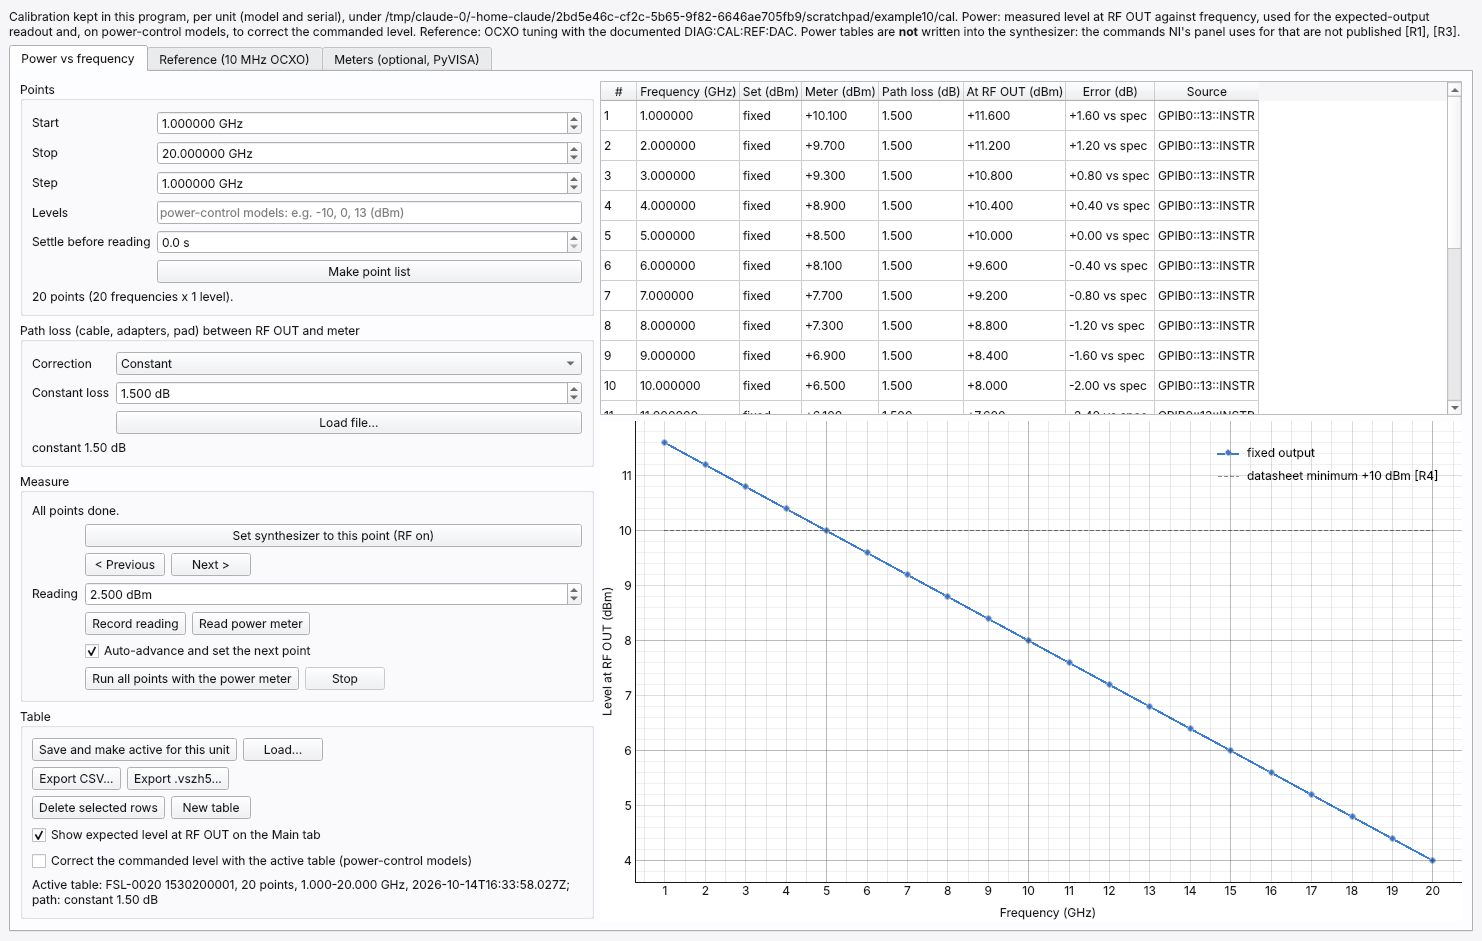
\includegraphics{examples/calibration_simulated_FSL-0020/calibration_tab_power.png}
\caption{Calibration tab, \emph{Power vs frequency} page, after a
\textbf{simulated} 20-point run on the FSL-0020 simulator (synthetic
level \(12-0.4\,f/\mathrm{GHz}\) dBm, 1.5 dB constant path loss). Not a
measurement.}
\end{figure}

\begin{figure}
\centering
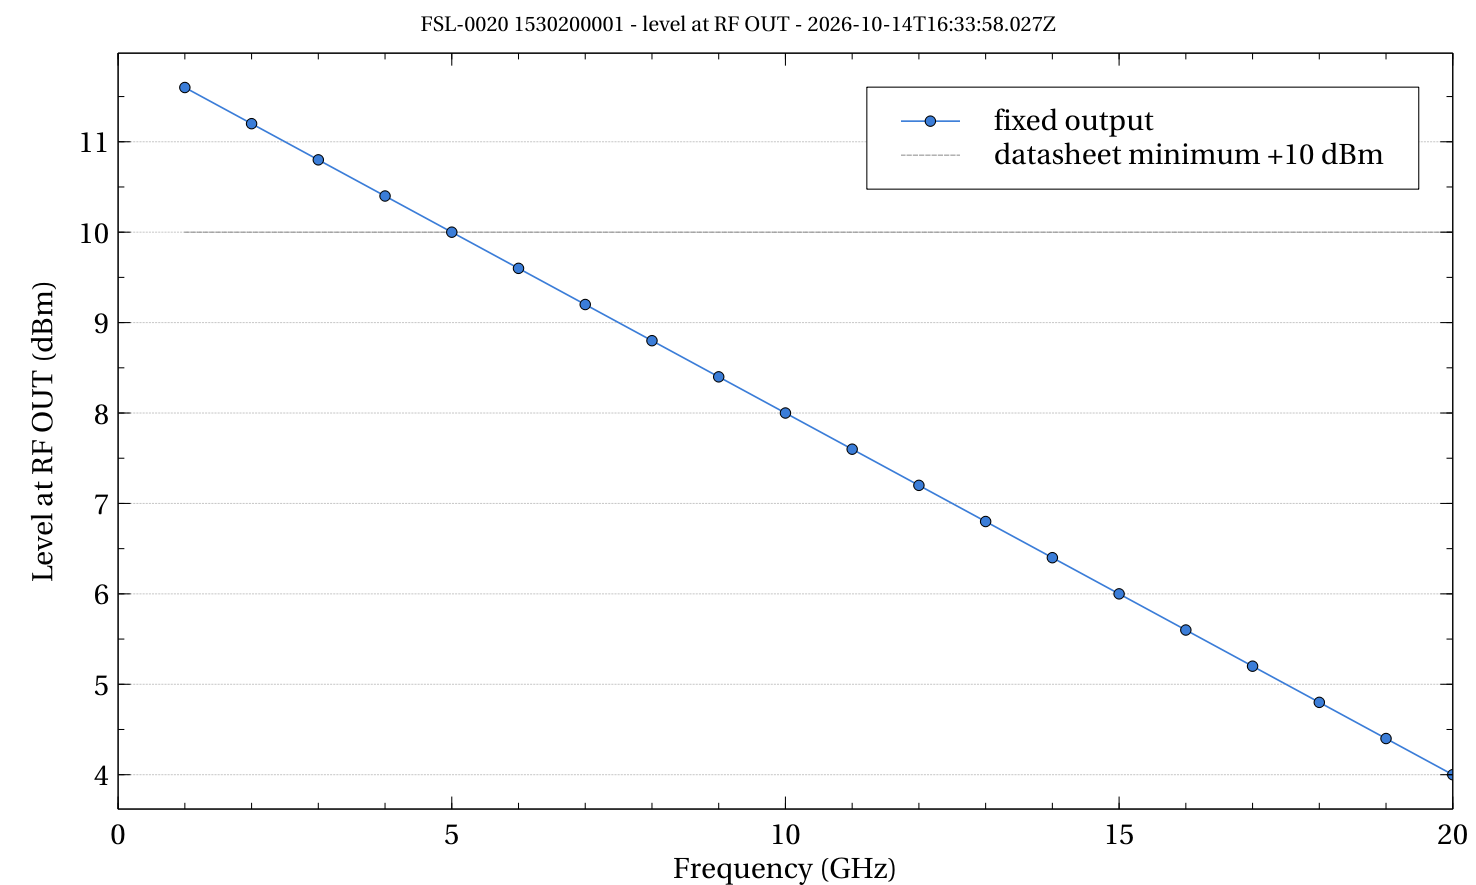
\includegraphics{examples/calibration_simulated_FSL-0020/power_cal_simulated_FSL-0020_p00_page_power_cal.png}
\caption{The same simulated table exported as \texttt{.vszh5} and
rendered by Veusz 4.2.1.}
\end{figure}

\hypertarget{the-64-byte-buffer-and-why-frequencies-are-encoded-two-ways}{%
\section{4. The 64-byte buffer, and why frequencies are encoded two
ways}\label{the-64-byte-buffer-and-why-frequencies-are-encoded-two-ways}}

Millihertz is the documented default unit for \texttt{FREQ} {[}1, Table
5{]}, and a standalone \texttt{FREQ} is sent that way because it is
exact and always fits. But a 20 GHz carrier is 14 characters in
millihertz, and

\begin{verbatim}
SWE:FAST:FREQ:SETUP 2000000000000,10000000000000,80,2.0dBm,1s,10,0,0
\end{verbatim}

is \textbf{69 bytes with its terminator} --- five over the device
buffer. This is why every compound example in {[}1{]} writes frequencies
with a \texttt{GHz} suffix. \texttt{format\_frequency()} therefore
returns the shortest \emph{exact} spelling among millihertz,
\texttt{KHz}, \texttt{MHz} and \texttt{GHz}:

\begin{longtable}[]{@{}
  >{\raggedright\arraybackslash}p{(\columnwidth - 4\tabcolsep) * \real{0.3333}}
  >{\raggedright\arraybackslash}p{(\columnwidth - 4\tabcolsep) * \real{0.3333}}
  >{\raggedright\arraybackslash}p{(\columnwidth - 4\tabcolsep) * \real{0.3333}}@{}}
\toprule\noalign{}
\begin{minipage}[b]{\linewidth}\raggedright
Requested
\end{minipage} & \begin{minipage}[b]{\linewidth}\raggedright
Encoded
\end{minipage} & \begin{minipage}[b]{\linewidth}\raggedright
Why
\end{minipage} \\
\midrule\noalign{}
\endhead
\bottomrule\noalign{}
\endlastfoot
2.000000000 GHz & \texttt{2GHz} & 4 bytes beats 13 \\
2.200000000 GHz & \texttt{2.2GHz} & matches the \texttt{FREQ\ 2.2GHz}
example in {[}1{]} \\
0.100000000 GHz & \texttt{0.1GHz} & 6 bytes beats \texttt{100MHz}, ties
go to GHz \\
9.111222333 GHz & \texttt{9111222333000} & 13 bytes beats
\texttt{9.111222333GHz} at 14 \\
\end{longtable}

The same sweep now encodes to 51 bytes. A command that still will not
fit --- three full-precision frequencies in a normal sweep, say --- is
refused \emph{before} transmission with advice on which parameter to
round, rather than being silently truncated by the device.

\begin{center}\rule{0.5\linewidth}{0.5pt}\end{center}

\hypertarget{logging}{%
\section{5. Logging}\label{logging}}

Each session creates
\texttt{\textless{}log\_root\textgreater{}/\textless{}YYYYmmdd\_HHMMSS\textgreater{}\_\textless{}model\textgreater{}\_\textless{}opts\textgreater{}/}:

\begin{longtable}[]{@{}
  >{\raggedright\arraybackslash}p{(\columnwidth - 2\tabcolsep) * \real{0.5000}}
  >{\raggedright\arraybackslash}p{(\columnwidth - 2\tabcolsep) * \real{0.5000}}@{}}
\toprule\noalign{}
\begin{minipage}[b]{\linewidth}\raggedright
Artefact
\end{minipage} & \begin{minipage}[b]{\linewidth}\raggedright
Contents
\end{minipage} \\
\midrule\noalign{}
\endhead
\bottomrule\noalign{}
\endlastfoot
\texttt{session\_metadata.json} & Identity, capability row, transport
settings, sampler configuration, record dtype, versions \\
\texttt{session.log} & Human-readable event log \\
\texttt{transactions.csv} &
\texttt{seq,\ iso\_utc,\ t\_unix,\ direction,\ command,\ response,\ latency\_ms,\ ok,\ error}
--- every byte exchanged \\
\texttt{state\_events.csv} &
\texttt{seq,\ iso\_utc,\ t\_unix,\ parameter,\ value,\ source} --- every
commanded change of generated-signal state \\
\texttt{telemetry.csv} & 25 columns: timestamps, frequency, power,
temperature, decoded status and modulation bits, latency, instantaneous
rate \\
\texttt{telemetry\_chunk\_\#\#\#\#.pkl.gz} & gzip-pickled NumPy blocks
of the same records, 52 bytes each (written via \texttt{.part} +
rename) \\
\texttt{quicksyn\_session.vszh5} & Veusz HDF5 document: all data and
plot pages (§6) --- written by the controller at stop, on demand, or
every N minutes \\
\end{longtable}

The log root is set on the \emph{Monitor and log} tab and defaults to
\texttt{quicksyn\_logs} in the home folder --- on the hardware PC,
\texttt{C:\textbackslash{}Users\textbackslash{}wwallace\textbackslash{}quicksyn\_logs\textbackslash{}20261012\_140204\_FSL-0020\_0000017f\textbackslash{}}
(the path is also the second line of \texttt{session.log}). NI's
QuickSyn soft front panel keeps no log file: its command window only
displays the commands of the session {[}2{]}; only \emph{Save List to
File} (List Mode) and the calibration panel's \emph{Save Data to File}
write files, to wherever their file dialog points {[}2{]}, {[}3{]}.

\texttt{transactions.csv} is the audit trail of \emph{what was sent};
\texttt{state\_events.csv} is the readable record of \emph{what was
generated}; \texttt{telemetry.csv} is \emph{what the instrument reported
back}, at the sample rate.

\hypertarget{sample-rate}{%
\subsection{5.1 Sample rate}\label{sample-rate}}

The requested period is

\[ \tau_0 = \frac{1}{f_s} \]

and each sample costs one serial round trip per enabled field. With
\(N_q\) queries per sample and mean round-trip time \(t_q\) the ceiling
is

\[ f_{s,\max} = \frac{1}{N_q\,t_q} \]

Polling frequency, power, status, modulation and temperature gives
\(N_q = 6\) --- temperature counts twice while the conservative
double-issue rule is enabled --- so at \(t_q \approx 8\) ms,

\[ f_{s,\max} \approx \frac{1}{6 \times 8\times10^{-3}} \approx 21\ \text{Hz} \]

The Monitor tab shows this budget live and turns it into a warning when
the requested rate exceeds it; the \textbf{achieved} rate and the serial
duty cycle are measured once per second, not estimated. Temperature
decimation (every \emph{N}th sample, default 5) buys the bandwidth back,
since the internal temperature moves on a thermal time constant of
minutes.

Scheduling is absolute: the deadline for sample \emph{k} is computed
from the acquisition start time as \(t_0 + k\,\tau_0\), so jitter in one
iteration does not accumulate into drift.

\hypertarget{memory-discipline}{%
\subsection{5.2 Memory discipline}\label{memory-discipline}}

\begin{longtable}[]{@{}
  >{\raggedright\arraybackslash}p{(\columnwidth - 2\tabcolsep) * \real{0.5000}}
  >{\raggedright\arraybackslash}p{(\columnwidth - 2\tabcolsep) * \real{0.5000}}@{}}
\toprule\noalign{}
\begin{minipage}[b]{\linewidth}\raggedright
Mechanism
\end{minipage} & \begin{minipage}[b]{\linewidth}\raggedright
Effect
\end{minipage} \\
\midrule\noalign{}
\endhead
\bottomrule\noalign{}
\endlastfoot
Preallocated NumPy ring buffer & Fixed RAM: \texttt{capacity\ ×\ 52}
bytes, allocated once (60 000 records ≈ 3.1 MB) \\
Spill on overflow & A full block is handed to the writer thread and the
index resets, so steady-state RAM is flat however long the run \\
Queue-decoupled writer thread & All disk I/O leaves the sampler thread;
a slow filesystem cannot distort the sample interval \\
\textbf{Flush RAM to disk now} & Spills the resident block on demand \\
Live accounting & Ring fill, buffer RAM, process RSS, writer queue depth
and chunk count on the Monitor tab \\
\end{longtable}

\hypertarget{parallelism-and-gpu}{%
\subsection{5.3 Parallelism and GPU}\label{parallelism-and-gpu}}

Device I/O cannot be parallelised --- the instrument is one half-duplex
endpoint behind a single reentrant lock. What \emph{is} parallel: the
sampler thread, the writer thread, and the GUI, plus process-pool chunk
loading and optional CuPy reductions in the companion script. The
controller uses no GPU on purpose: at a \textasciitilde20 Hz ceiling the
host-device transfer would cost more than the arithmetic it replaces.

\hypertarget{live-scpi-console}{%
\subsection{5.4 Live SCPI console}\label{live-scpi-console}}

\textbf{View ▸ SCPI console} (\textbf{Ctrl+Shift+C}) shows every
exchange with the instrument as it happens, in a pane docked under the
tabs with room for about ten lines. It can be resized with the splitter,
undocked, moved to any edge or closed, and opens again from the View
menu. To make that room, the tab pages now scroll when the window is
shorter than a page: in 0.0.4 the tallest page (Monitor and log) forced
a minimum window height of 981 px, which would not fit a small laptop
screen. The window opens at 1180 × 960 px, or smaller if the screen is.

\begin{verbatim}
19:45:19.229 GUI  → POW -3.0  (write, 0.6 ms)
19:45:19.231 GUI  → FREQ?
                  ← 12500000000000  (1.6 ms)
19:45:21.652 GUI  → FREQ 9876543210000  (write, 0.6 ms)
19:45:21.653 GUI  → POW?
                  ✖ empty response (timeout)  (500.0 ms)
19:45:22.643 POLL → FREQ?
                  ← 9876543210000  (1.6 ms)
\end{verbatim}

(Lines copied from the 0.0.6 console in a simulated session; the timeout
was injected. The \texttt{POLL} line is visible because \emph{Show
telemetry polls} was ticked.) After a long pause with polls shown, the
redraw starts with one grey line, for example after 200 200 exchanges:

\begin{verbatim}
⋯ 197700 earlier exchanges not shown here (the console keeps the newest 5000 lines); the session's transactions.csv holds every exchange while logging
\end{verbatim}

Each line starts with the local time to the millisecond and the source.
A command that expects no reply is one line with its write time; a query
is the command and, under it, the reply or the error.

\begin{longtable}[]{@{}
  >{\raggedright\arraybackslash}p{(\columnwidth - 4\tabcolsep) * \real{0.3333}}
  >{\raggedright\arraybackslash}p{(\columnwidth - 4\tabcolsep) * \real{0.3333}}
  >{\raggedright\arraybackslash}p{(\columnwidth - 4\tabcolsep) * \real{0.3333}}@{}}
\toprule\noalign{}
\begin{minipage}[b]{\linewidth}\raggedright
Element
\end{minipage} & \begin{minipage}[b]{\linewidth}\raggedright
Meaning
\end{minipage} & \begin{minipage}[b]{\linewidth}\raggedright
Colour
\end{minipage} \\
\midrule\noalign{}
\endhead
\bottomrule\noalign{}
\endlastfoot
\texttt{→} & Command sent, exactly as transmitted (terminator not shown)
& blue \\
\texttt{←} & Reply received, with the round-trip latency & green \\
\texttt{✖} & Timeout or I/O error, with the reason & red \\
\texttt{GUI} / \texttt{POLL} & Issued by you (any tab or menu) / by the
telemetry sampler & grey / amber \\
\end{longtable}

The colours are mid-tones chosen to stay legible in the light and dark
themes.

\begin{longtable}[]{@{}
  >{\raggedright\arraybackslash}p{(\columnwidth - 2\tabcolsep) * \real{0.5000}}
  >{\raggedright\arraybackslash}p{(\columnwidth - 2\tabcolsep) * \real{0.5000}}@{}}
\toprule\noalign{}
\begin{minipage}[b]{\linewidth}\raggedright
Control
\end{minipage} & \begin{minipage}[b]{\linewidth}\raggedright
Effect
\end{minipage} \\
\midrule\noalign{}
\endhead
\bottomrule\noalign{}
\endlastfoot
\textbf{Show telemetry polls} & Off by default: at 10--20 Hz the
sampler's \texttt{FREQ?}/\texttt{POW?}/\texttt{STAT?} traffic would bury
your own commands. Polls are still counted and still logged to
\texttt{transactions.csv}; ticking the box redraws the retained history
with them \\
\textbf{Filter} & Shows only exchanges whose command, reply or error
contains the text, e.g.~\texttt{POW} or \texttt{LIST}. Applied when
typing pauses for 250 ms, or at once on \textbf{Enter}. While paused it
searches the frozen view \\
\textbf{Pause} / \textbf{Resume} & Freezes the view; exchanges keep
arriving and the newest appear on \textbf{Resume}. A pause of any length
costs no extra memory, and Resume draws at most the 5000 lines the view
can hold, with a grey \texttt{⋯} line counting anything older \\
\textbf{Auto-scroll} & Follows the newest line while the view is at the
bottom \\
\textbf{Copy} / \textbf{Save\ldots{}} / \textbf{Clear} & Copy the view,
save it as a \texttt{.txt} file, forget everything shown \\
\end{longtable}

The status line counts exchanges, polls and errors since the last clear.

How it is built. The driver reports every transaction through a Qt
signal; exchanges made on the sampler thread cross to the GUI thread as
queued signals (the slot runs when control returns to the GUI thread's
event loop {[}24{]}), so no widget is touched from a worker thread.
Receiving an exchange only files it, in constant time. A 150 ms timer
draws whatever is new, so a 20 Hz poll stream costs about seven redraws
per second, not one per exchange. Lines go in through a
\texttt{QTextCursor} with one character format per colour {[}25{]},
measured at 11--21 µs per line against 142--186 µs for
\texttt{appendHtml} (5000--10 000 lines); that is also why replies line
up exactly under their commands, where HTML had collapsed the space
after \texttt{GUI}.

Bounds, whatever the session length and however long the view is paused:

\begin{longtable}[]{@{}
  >{\raggedright\arraybackslash}p{(\columnwidth - 4\tabcolsep) * \real{0.3333}}
  >{\raggedright\arraybackslash}p{(\columnwidth - 4\tabcolsep) * \real{0.3333}}
  >{\raggedright\arraybackslash}p{(\columnwidth - 4\tabcolsep) * \real{0.3333}}@{}}
\toprule\noalign{}
\begin{minipage}[b]{\linewidth}\raggedright
Bound
\end{minipage} & \begin{minipage}[b]{\linewidth}\raggedright
Value
\end{minipage} & \begin{minipage}[b]{\linewidth}\raggedright
Why
\end{minipage} \\
\midrule\noalign{}
\endhead
\bottomrule\noalign{}
\endlastfoot
Lines in the view & 5000 (oldest removed first by
\texttt{maximumBlockCount} {[}23{]}) & The text widget's own memory and
layout cost \\
Exchanges kept for re-filtering & 20 000 \textbf{per source} (GUI and
POLL) & Polls can never push your own commands out of what the filter
searches \\
Lines drawn per redraw & ≤ 5000, the rest summarised in one \texttt{⋯}
line & Resume after any pause, or a filter change, blocks the window for
well under a second \\
Memory while paused & measured 5.3 MB for 200 200 exchanges (0.0.5: 45.5
MB, growing without limit) & Nothing is queued: Resume draws from the
two stores \\
\end{longtable}

0.0.5 queued every exchange that arrived during a pause and drew all of
them on Resume. At the default 2 Hz sample rate (3.4 queries per sample)
200 000 exchanges is about 8 hours of pause; at the nominal 50 Hz
maximum, about 20 minutes. Measured on the same simulated window:

\begin{longtable}[]{@{}
  >{\raggedright\arraybackslash}p{(\columnwidth - 4\tabcolsep) * \real{0.3333}}
  >{\raggedright\arraybackslash}p{(\columnwidth - 4\tabcolsep) * \real{0.3333}}
  >{\raggedright\arraybackslash}p{(\columnwidth - 4\tabcolsep) * \real{0.3333}}@{}}
\toprule\noalign{}
\begin{minipage}[b]{\linewidth}\raggedright
200 200 exchanges while paused
\end{minipage} & \begin{minipage}[b]{\linewidth}\raggedright
0.0.5
\end{minipage} & \begin{minipage}[b]{\linewidth}\raggedright
0.0.6
\end{minipage} \\
\midrule\noalign{}
\endhead
\bottomrule\noalign{}
\endlastfoot
Python memory held (tracemalloc) & 45.5 MB (unbounded) & 5.3 MB
(bounded) \\
Resume, polls hidden & 0.16 s & 0.01 s \\
Resume, polls shown & \textbf{62 s} with the window frozen & 0.07 s \\
Typing three filter characters, full store & 4.7 s of redraws & one
redraw after the typing pause \\
Command / reply arrow columns & \texttt{GUI} 17 / 18 (one off),
\texttt{POLL} 18 / 18 & 18 / 18 for both \\
\end{longtable}

The console is a live view, \textbf{not} the record ---
\texttt{transactions.csv} (§5) remains the complete audit trail of every
byte exchanged, and the \texttt{⋯} line says so.

From 0.0.7 the console also has a \emph{Send} line for typing commands
(§3.3), and warnings from the controller (a level that did not change,
an RF OFF that \texttt{STAT?} does not confirm) appear in it as red
\texttt{NOTE\ !} lines.

\begin{center}\rule{0.5\linewidth}{0.5pt}\end{center}

\hypertarget{auto-read-of-all-settings}{%
\subsection{5.5 Auto-read of all
settings}\label{auto-read-of-all-settings}}

\emph{Auto-read all settings every N s} (Main tab, under \emph{Read all
settings from instrument}; 1--3600 s, default 5 s) repeats the full
read-back on a timer while connected: frequency, level, \texttt{STAT?},
temperature, reference source, \texttt{OUTP:ROSC:STAT?} (where answered)
and modulation. A box being typed in is not overwritten. Three failed
reads in a row stop it with a warning, and it stops on disconnect. It
runs on the GUI thread and shares the port lock with the telemetry
sampler, so each read costs about nine exchanges; at 5 s that is under 2
exchanges per second. It updates the display only; the telemetry log is
still the sampler's.

\hypertarget{veusz-documents-reduction-and-plots}{%
\section{6. Veusz documents, reduction and
plots}\label{veusz-documents-reduction-and-plots}}

\begin{Shaded}
\begin{Highlighting}[]
\ExtensionTok{python}\NormalTok{ quicksyn\_veusz\_export\_v0\_0\_10.py }\OperatorTok{\textless{}}\NormalTok{session\_dir}\OperatorTok{\textgreater{}}
    \ExtensionTok{{-}{-}time{-}axis}\NormalTok{ A      local }\ErrorTok{(}\ExtensionTok{default}\KeywordTok{)}\ExtensionTok{,}\NormalTok{ utc or elapsed}
    \ExtensionTok{{-}{-}no{-}render}\NormalTok{        write the .vszh5 but skip the PDF/PNG render}
    \ExtensionTok{{-}{-}png{-}pages}\NormalTok{ P      first }\ErrorTok{(}\ExtensionTok{default,}\NormalTok{ the overview}\KeywordTok{)}\ExtensionTok{,}\NormalTok{ all or none}
    \ExtensionTok{{-}{-}veusz{-}exe}\NormalTok{ PATH   Veusz program for rendering }\ErrorTok{(}\ExtensionTok{default:}\NormalTok{ search}\KeywordTok{)}
    \ExtensionTok{{-}{-}render{-}method}\NormalTok{ M  auto }\ErrorTok{(}\ExtensionTok{default}\KeywordTok{)}\ExtensionTok{,}\NormalTok{ program or inprocess}
    \ExtensionTok{{-}{-}no{-}compress}\NormalTok{      store .vszh5 datasets uncompressed}
    \ExtensionTok{{-}{-}no{-}veusz}\NormalTok{         statistics only: no .vszh5, no plots}
    \ExtensionTok{{-}{-}no{-}gpu}\NormalTok{           force the NumPy host path}
    \ExtensionTok{{-}{-}workers}\NormalTok{ N        process{-}pool size }\ErrorTok{(}\ExtensionTok{default:}\NormalTok{ CPUs this process may use}\KeywordTok{)}
    \ExtensionTok{{-}{-}dpi}\NormalTok{ N            PNG resolution }\ErrorTok{(}\ExtensionTok{default}\NormalTok{ 150}\KeywordTok{)}
    \ExtensionTok{{-}{-}no{-}latex}\NormalTok{         do not write or compile the LuaLaTeX report}
    \ExtensionTok{{-}{-}lualatex}\NormalTok{ PATH    lualatex to use }\ErrorTok{(}\ExtensionTok{default:}\NormalTok{ search, see section 6.7}\KeywordTok{)}
    \ExtensionTok{{-}{-}version,} \AttributeTok{{-}V}\NormalTok{      print version, copyright and licence, then exit}
\end{Highlighting}
\end{Shaded}

Writes \texttt{reduction\_summary.json}, \texttt{reduction\_summary.md}
(Obsidian-ready, LaTeX equations), \texttt{telemetry\_reduced.npz}, and
\textbf{\texttt{quicksyn\_session.vszh5}}, a native Veusz HDF5 document
written directly with \texttt{h5py} --- \textbf{Veusz is not needed to
create it}. Open it in Veusz (File ▸ Open) to restyle the plots. When
Veusz is installed, \texttt{quicksyn\_session.pdf} (every page, with a
bookmark hierarchy) and page PNGs are rendered \emph{from} the
\texttt{.vszh5}, which also proves it opens, and the LuaLaTeX report
\texttt{quicksyn\_session\_report.tex} is written and, when
\texttt{lualatex} is found, compiled to
\texttt{quicksyn\_session\_report.pdf} (§6.7). No text \texttt{.vsz} is
ever written. The controller produces the same files itself (§6.4).

\hypertarget{why-.vszh5-and-not-.vsz}{%
\subsection{\texorpdfstring{6.1 Why \texttt{.vszh5} and not
\texttt{.vsz}}{6.1 Why .vszh5 and not .vsz}}\label{why-.vszh5-and-not-.vsz}}

A text \texttt{.vsz} stores embedded data with
\texttt{fmt=\textquotesingle{}\%e\textquotesingle{}} {[}18{]}, i.e.~as
\(m \times 10^{k}\) with \(1 \le m < 10\) printed to six decimals: seven
significant digits. The exporter stores the carrier in GHz, so with
\(k = \lfloor \log_{10} f_{\mathrm{GHz}} \rfloor\) the quantisation step
and the worst-case rounding error are

\[q = 10^{\,k-6}\ \text{GHz}, \qquad |\varepsilon| \le \frac{q}{2},
\qquad \frac{|\varepsilon|}{f} \le \frac{q/2}{10^{k}} = 5\times10^{-7}.\]

\begin{longtable}[]{@{}llll@{}}
\toprule\noalign{}
Carrier & \(k\) & Step \(q\) & Worst-case error \\
\midrule\noalign{}
\endhead
\bottomrule\noalign{}
\endlastfoot
1 to \textless{} 10 GHz & 0 & 1 kHz & 500 Hz \\
10 to \textless{} 100 GHz & 1 & 10 kHz & 5 kHz \\
\end{longtable}

Measured on 200 000 random carriers per decade: maximum 500.0 Hz and
5000.0 Hz, as predicted. Examples: 9.876543210 GHz came back 210 Hz off,
11.123456789 GHz 3211 Hz off, and two carriers 1 mHz apart merged. The
\texttt{.vszh5} stores IEEE-754 float64 verbatim (53-bit significand,
\(\approx 1.1\times10^{-16}\) relative), so every value round-trips
bit-exact.

\hypertarget{the-writer-vszh5_writer.py-from-isp_speed_monitor.py}{%
\subsection{\texorpdfstring{6.2 The writer: \texttt{vszh5\_writer.py}
(from
\texttt{isp\_speed\_monitor.py})}{6.2 The writer: vszh5\_writer.py (from isp\_speed\_monitor.py)}}\label{the-writer-vszh5_writer.py-from-isp_speed_monitor.py}}

The Veusz file creation is the method from the author's
\texttt{isp\_speed\_monitor.py} 1.3.0 {[}21{]}, moved into its own
module so both the controller and the export script use one
implementation, and so it can be reused in other programs. Your call
signatures are kept.

\begin{longtable}[]{@{}
  >{\raggedright\arraybackslash}p{(\columnwidth - 4\tabcolsep) * \real{0.3333}}
  >{\raggedright\arraybackslash}p{(\columnwidth - 4\tabcolsep) * \real{0.3333}}
  >{\raggedright\arraybackslash}p{(\columnwidth - 4\tabcolsep) * \real{0.3333}}@{}}
\toprule\noalign{}
\begin{minipage}[b]{\linewidth}\raggedright
Item
\end{minipage} & \begin{minipage}[b]{\linewidth}\raggedright
Origin
\end{minipage} & \begin{minipage}[b]{\linewidth}\raggedright
What it does
\end{minipage} \\
\midrule\noalign{}
\endhead
\bottomrule\noalign{}
\endlastfoot
\texttt{VeuszWriter} & \texttt{VeuszWriter} & Opens
\texttt{\textless{}file\textgreater{}.part}, writes \texttt{/Veusz} with
\texttt{vsz\_format\ =\ 1}, typed datasets (\texttt{dataset\_1d} with
\texttt{serr}, plus \texttt{perr}/\texttt{nerr}; \texttt{dataset\_date};
\texttt{dataset\_text}) and tags; \texttt{finish()} stores the script
and renames atomically \\
\texttt{VszDoc} & \texttt{VszDoc} & Builds the Veusz command script:
\texttt{add}, \texttt{to}, \texttt{up}, \texttt{set} (paths like
\texttt{x/label}) \\
\texttt{vz\_text()} & \texttt{vz\_text()} & Escapes label text --- now
identical to Veusz \texttt{latexEscape} \\
\texttt{epoch\_to\_veusz()}, \texttt{local\_utc\_offsets()} &
\texttt{epoch\_to\_veusz()} & Unix seconds → Veusz dates (s since
2009-01-01); per-sample UTC offset, DST-aware \\
\texttt{find\_veusz\_exe()} & \texttt{find\_veusz\_exe()} &
\texttt{QUICKSYN\_VEUSZ} / \texttt{VEUSZ\_EXE}, PATH, then the usual
install folders \\
\texttt{render\_pages()} & \texttt{tests/render\_in\_veusz.sh} & Drives
the Veusz program in \texttt{-\/-listen} mode with \texttt{loadHDF5Doc};
PDF of every page and per-page PNGs; falls back to the Veusz Python
package when the program is absent or fails; bookmarks the PDF \\
\texttt{add\_pdf\_bookmarks()} & new in 0.0.6 & Writes a bookmark
hierarchy and document information into a PDF with pypdf, atomically,
and opens the bookmark pane \\
\end{longtable}

Changes from 1.3.0, each found by testing against real Veusz:

\begin{longtable}[]{@{}
  >{\raggedright\arraybackslash}p{(\columnwidth - 2\tabcolsep) * \real{0.5000}}
  >{\raggedright\arraybackslash}p{(\columnwidth - 2\tabcolsep) * \real{0.5000}}@{}}
\toprule\noalign{}
\begin{minipage}[b]{\linewidth}\raggedright
Change
\end{minipage} & \begin{minipage}[b]{\linewidth}\raggedright
Reason
\end{minipage} \\
\midrule\noalign{}
\endhead
\bottomrule\noalign{}
\endlastfoot
\texttt{vz\_text} maps \texttt{\textbackslash{}} to
\texttt{\{\textbackslash{}backslash\}} and escapes \texttt{{[}}
\texttt{{]}} & In Veusz text \texttt{\textbackslash{}\textbackslash{}}
is a \textbf{line break} {[}18, \texttt{textrender.py}{]}, so the 1.3.0
escape split a label at any backslash (a Windows path in a title) \\
Atomic \texttt{.part} write, \texttt{abort()} and a context manager
built into the class & An exception mid-write discards the partial file;
the previous complete file stays \\
Optional gzip + shuffle & 8-hour sessions; Veusz reads compressed
datasets transparently \\
\texttt{render\_pages} waits for a done marker, then ends Veusz & Veusz
4.2.1 does \textbf{not exit} on \texttt{Quit()} in listen mode (3.6.2
does); \texttt{render\_in\_veusz.sh} would sit until its
\texttt{timeout\ 180} \\
Paths in the render script go through \texttt{repr()} & Windows
back-slashes in an interpolated path would become escape sequences \\
\textbf{0.0.5:} the PNG path is bound on its own line, outside the
\texttt{exec()} string & 0.0.4 put it inside the \texttt{exec()} string,
where it was unescaped a second time:
\texttt{C:\textbackslash{}Users\textbackslash{}…} failed to compile,
\texttt{C:\textbackslash{}data\textbackslash{}new} gained a newline, and
a quote in the path broke the string. Found while fixing the same code
in the speed monitor \\
\textbf{0.0.5:} \texttt{method="auto"} falls back to the Python package
when the program \emph{fails}, not only when it is missing & A Veusz on
the PATH can be present but broken: Ubuntu's \texttt{/usr/bin/veusz}
starts \texttt{/usr/bin/python3}, and when that has been switched to
another Python than the one the package was built for (3.13 instead of
3.12 in the test machine) it stops with
\texttt{No\ module\ named\ \textquotesingle{}PyQt5.sip\textquotesingle{}}.
Both errors are reported if the fallback fails too \\
\textbf{0.0.5:} a program that exits before reading its script, or
cannot be started, is a failed render & It raised
\texttt{BrokenPipeError} or \texttt{OSError} instead of
\texttt{RuntimeError}, which skipped the fallback; a race, so it only
showed up sometimes \\
\textbf{0.0.6:} PDFs are exported with \texttt{pdfdpi=72} & Veusz 4.2.1
drew every PDF page in the top-left 48 \% of the page (§6.5). The PNGs
were always right, and the 0.0.4 checks inspected PNGs, so it went
unnoticed until the PDFs were bookmarked and included in the LaTeX
report \\
\textbf{0.0.6:} the PDF gets a bookmark hierarchy & Session ▸ Overview,
Time series (one entry per quantity), Stability (§6.7) \\
\textbf{0.0.6:} a re-render reports its files & 0.0.5 compared against
the folder listing taken before the render, so rendering a second time
into the same folder returned nothing and the controller showed no
plots \\
\end{longtable}

\hypertarget{what-the-session-document-contains}{%
\subsection{6.3 What the session document
contains}\label{what-the-session-document-contains}}

\begin{longtable}[]{@{}
  >{\raggedright\arraybackslash}p{(\columnwidth - 4\tabcolsep) * \real{0.3333}}
  >{\raggedright\arraybackslash}p{(\columnwidth - 4\tabcolsep) * \real{0.3333}}
  >{\raggedright\arraybackslash}p{(\columnwidth - 4\tabcolsep) * \real{0.3333}}@{}}
\toprule\noalign{}
\begin{minipage}[b]{\linewidth}\raggedright
Datasets
\end{minipage} & \begin{minipage}[b]{\linewidth}\raggedright
Tag
\end{minipage} & \begin{minipage}[b]{\linewidth}\raggedright
Contents
\end{minipage} \\
\midrule\noalign{}
\endhead
\bottomrule\noalign{}
\endlastfoot
\texttt{raw/time\_utc}, \texttt{raw/time\_local} & raw & Veusz dates of
every sample (local follows DST) \\
\texttt{raw/elapsed\_s}, \texttt{raw/epoch\_s},
\texttt{raw/utc\_offset\_s}, \texttt{raw/index} & raw & Time bases and
sample index \\
\texttt{raw/freq\_hz}, \texttt{raw/freq\_ghz}, \texttt{raw/power\_dbm},
\texttt{raw/temp\_c} & raw & Reported carrier, level, internal
temperature \\
\texttt{raw/latency\_ms}, \texttt{raw/interval\_ms},
\texttt{raw/rate\_hz} & raw & I/O latency, sample interval, requested
rate \\
\texttt{raw/status\_word}, \texttt{raw/modulation\_word},
\texttt{raw/rf\_on}, \texttt{raw/rf\_unlocked},
\texttt{raw/ref\_unlocked}, \texttt{raw/voltage\_error} & raw &
\texttt{STAT?} / \texttt{DIAG:MOD?} words and decoded flags \\
\texttt{events/*} (times, \texttt{parameter}, \texttt{value},
\texttt{source}, \texttt{freq\_ghz}, \texttt{power\_dbm}) & events &
Every commanded change from \texttt{state\_events.csv} \\
\texttt{stability/tau\_s}, \texttt{stability/adev} & stability &
Overlapping ADEV of the reported carrier \\
\texttt{meta/session}, \texttt{meta/session\_metadata\_json},
\texttt{meta/reduction\_summary\_json}, \texttt{meta/generator} & meta &
Provenance \\
\end{longtable}

\begin{longtable}[]{@{}
  >{\raggedright\arraybackslash}p{(\columnwidth - 2\tabcolsep) * \real{0.5000}}
  >{\raggedright\arraybackslash}p{(\columnwidth - 2\tabcolsep) * \real{0.5000}}@{}}
\toprule\noalign{}
\begin{minipage}[b]{\linewidth}\raggedright
Page
\end{minipage} & \begin{minipage}[b]{\linewidth}\raggedright
Contents
\end{minipage} \\
\midrule\noalign{}
\endhead
\bottomrule\noalign{}
\endlastfoot
\texttt{page\_overview} & 3 × 2 grid: carrier, level, temperature,
latency, sample interval, ADEV \\
\texttt{page\_carrier}, \texttt{page\_level} & Reported trace with
\textbf{commanded values overlaid as markers} \\
\texttt{page\_thermal}, \texttt{page\_latency}, \texttt{page\_interval}
& One quantity per page against the chosen time axis \\
\texttt{page\_stability} & Log--log ADEV \\
\end{longtable}

\hypertarget{from-the-controller}{%
\subsection{6.4 From the controller}\label{from-the-controller}}

The controller writes the \texttt{.vszh5} itself --- no separate step:

\begin{longtable}[]{@{}
  >{\raggedright\arraybackslash}p{(\columnwidth - 2\tabcolsep) * \real{0.5000}}
  >{\raggedright\arraybackslash}p{(\columnwidth - 2\tabcolsep) * \real{0.5000}}@{}}
\toprule\noalign{}
\begin{minipage}[b]{\linewidth}\raggedright
Trigger
\end{minipage} & \begin{minipage}[b]{\linewidth}\raggedright
Where
\end{minipage} \\
\midrule\noalign{}
\endhead
\bottomrule\noalign{}
\endlastfoot
Logging stops (default on) & Monitor tab ▸ Veusz document ▸ \emph{Write
when logging stops} \\
On demand, during or after logging & \emph{Write .vszh5 now}, Veusz
menu, \textbf{Ctrl+E} \\
Every N minutes while logging & Monitor tab ▸ \emph{Refresh while
logging} (0 = off) \\
PDF/PNG and the LuaLaTeX report as well & \emph{Also render PDF/PNG with
Veusz}, or Veusz ▸ \emph{Write .vszh5 and render}; the status bar names
the plots and the report \\
View & \emph{Open in Veusz} (uses \texttt{find\_veusz\_exe}, else the
desktop file association) \\
\end{longtable}

The export runs the companion script \textbf{as a separate process}: the
GUI's PySide6 never shares a process with the Qt binding Veusz uses, a
long session never stalls the window, and the export started by closing
the window runs detached and finishes after the window is gone. While
logging, the RAM ring is spilled first and the writer thread allowed to
commit it, so the document holds every sample up to that moment;
telemetry chunks are now written to \texttt{.part} and renamed, so a
concurrent export never reads half a chunk.

\hypertarget{rendering-and-veusz-command-line-limitations}{%
\subsection{6.5 Rendering, and Veusz command-line
limitations}\label{rendering-and-veusz-command-line-limitations}}

Tested with Veusz 3.6.2 and 4.2.1:

\begin{itemize}
\tightlist
\item
  \texttt{veusz\ -\/-export=out.pdf\ file.vszh5} \textbf{cannot} open a
  \texttt{.vszh5}: the command line loads every file as a text script,
  gets an empty document, and the export fails. The embedded interface's
  \texttt{Load} command has the same limit.
\item
  \texttt{-\/-export-dpi} is not a Veusz option (exit code 2), and
  \texttt{\%PAGE\%} page templates are expanded only by the GUI's Export
  dialog, not the command line.
\item
  Veusz 4.2.1 does not exit on \texttt{Quit()} in
  \texttt{-\/-listen\ -\/-quiet} mode (3.6.2 does), so
  \texttt{render\_pages()} waits for its own end marker, gives Veusz two
  seconds, then ends it.
\item
  Veusz 4.2.1 draws a scripted PDF at 72/150 of its size, in the
  top-left corner of each page. \texttt{AsyncExport.getDPI()} rounds the
  PDF resolution to the only one Qt's PDF engine reports (72) and lays
  the page out at it, but \texttt{ExportPDFRunnable} sets the printer to
  the requested \texttt{pdfdpi}, and \texttt{Export()} defaults to 150
  {[}18{]}, {[}22{]}. Veusz 3.6.2 did not round, so it is correct.
  \texttt{render\_pages()} passes \texttt{pdfdpi=72}, which is right for
  both.
\item
  What works: \texttt{veusz\ -\/-listen\ -\/-quiet} fed a script that
  calls \texttt{veusz.document.loader.loadHDF5Doc} and
  \texttt{Export(...,\ page={[}i{]})}, which is what
  \texttt{render\_pages()} does, or the Python package's
  \texttt{Document.load(path,\ mode=\textquotesingle{}hdf5\textquotesingle{})}.
\end{itemize}

\textbf{Fixing it in Veusz.} All three limits come from short functions
in Veusz itself {[}18{]}, unchanged on its \texttt{master} branch as of
2026-10-11 {[}22{]}:

\begin{enumerate}
\def\labelenumi{\arabic{enumi}.}
\tightlist
\item
  \texttt{CommandInterpreter.Load()} opens every file as UTF-8 text, and
  both the command line and the embedding API go through it.
\item
  The listen loop's \texttt{quitProgram()} only closes a window that
  \texttt{-\/-quiet} never showed. Qt ends the application on
  \texttt{lastWindowClosed}, which is emitted only for the last
  \emph{visible} window {[}29{]}.
\item
  \texttt{ExportPDFRunnable} sets the printer to \texttt{pdfdpi} rather
  than to the resolution the page was laid out at.
\end{enumerate}

The patch \texttt{upstream/veusz-4.2.1-vszh5-load-quit-pdfdpi.patch}
makes \texttt{Load()} recognise an HDF5 file by its signature and open
it with \texttt{mode=\textquotesingle{}hdf5\textquotesingle{}}, makes
\texttt{quitProgram()} also quit the application, and sets the PDF
printer to the layout resolution. A ready-to-file issue text is in
\texttt{upstream/VEUSZ\_UPSTREAM\_ISSUE.md}.

\texttt{upstream/check\_veusz\_patch.py} reproduces all three on any set
of Veusz programs. ``Text reaches'' is the rightmost text on page 1 as a
fraction of the page width; about 0.97 means the drawing fills the page.

\begin{longtable}[]{@{}
  >{\raggedright\arraybackslash}p{(\columnwidth - 6\tabcolsep) * \real{0.2500}}
  >{\raggedright\arraybackslash}p{(\columnwidth - 6\tabcolsep) * \real{0.2500}}
  >{\raggedright\arraybackslash}p{(\columnwidth - 6\tabcolsep) * \real{0.2500}}
  >{\raggedright\arraybackslash}p{(\columnwidth - 6\tabcolsep) * \real{0.2500}}@{}}
\toprule\noalign{}
\begin{minipage}[b]{\linewidth}\raggedright
Check
\end{minipage} & \begin{minipage}[b]{\linewidth}\raggedright
4.2.1
\end{minipage} & \begin{minipage}[b]{\linewidth}\raggedright
4.2.1 + patch
\end{minipage} & \begin{minipage}[b]{\linewidth}\raggedright
3.6.2
\end{minipage} \\
\midrule\noalign{}
\endhead
\bottomrule\noalign{}
\endlastfoot
\texttt{-\/-export} \texttt{.vszh5} to PDF & fails (exit −11,
segmentation fault, no file) & OK, text reaches 0.97 & fails (exit 0, no
file) \\
\texttt{-\/-export} \texttt{.vszh5} to PNG & fails (exit −11, no file) &
OK & fails (exit 0, no file) \\
\texttt{Load()} \texttt{.vszh5} + \texttt{Export()} of 2 pages & fails
(no PDF) & OK, 2 pages, text reaches 0.97 & fails (no PDF) \\
\texttt{Quit()} in \texttt{-\/-listen\ -\/-quiet} & still running 30 s
after \texttt{DONE} (killed) & exits 0.12 s after \texttt{DONE} & exits
0.11 s after \texttt{DONE} \\
Text \texttt{.vsz} \texttt{-\/-export} to PDF (regression) & OK, but
text reaches \textbf{0.47} & OK, text reaches 0.97 & OK, text reaches
0.97 \\
This package's \texttt{check\_vszh5.py} & 58 / 58 & 58 / 58 & 58 / 58 \\
\end{longtable}

The patch is for submitting upstream {[}22{]}; this package does
\textbf{not} need it. \texttt{render\_pages()} uses the listen-mode
route and \texttt{pdfdpi=72}, which work with patched and unpatched
Veusz alike.

\hypertarget{statistics}{%
\subsection{6.6 Statistics}\label{statistics}}

Reported statistics include achieved rate, interval jitter, I/O latency
percentiles, distinct commanded frequencies, power and temperature
extrema, margin to the +75 °C internal limit {[}2{]}, lock-loss and
voltage-error tallies, and the overlapping Allan deviation of the
reported carrier per IEEE Std 1139-2008 {[}9{]}:

\[ \sigma_y^2(\tau) = \frac{1}{2\,(N-2m+1)\,\tau^2}
   \sum_{k=1}^{N-2m+1}\left(x_{k+2m} - 2x_{k+m} + x_k\right)^2,
   \qquad \tau = m\,\tau_0 \]

with phase residuals \(x_k = \tau_0\sum_{i<k} y_i\) and fractional error
\(y_i = (f_i - f_c)/f_c\). Evaluating it from cumulative sums turns the
inner double sum from \(\mathcal{O}(Nm)\) into \(\mathcal{O}(N)\) per
averaging factor; the result was cross-checked against a direct
summation and agrees to better than \(10^{-9}\) relative.

\begin{quote}
\textbf{Read this statistic correctly.} \texttt{FREQ?} returns the
\emph{commanded} setting, not a measurement of the output. The ADEV here
characterises command fidelity and the logging time base --- a non-zero
value means commands were lost, retimed or applied late. It is
\textbf{not} carrier phase noise, which is specified separately in
{[}4{]} and cannot be inferred from this log. Measuring the carrier
needs a counter or a phase-noise analyser.
\end{quote}

\hypertarget{pdf-bookmarks-and-the-lualatex-session-report}{%
\subsection{6.7 PDF bookmarks and the LuaLaTeX session
report}\label{pdf-bookmarks-and-the-lualatex-session-report}}

\textbf{Bookmarks in the rendered PDF.} \texttt{render\_pages()} writes
the outline with \texttt{vszh5\_writer.add\_pdf\_bookmarks()} (pypdf
{[}26{]}) after Veusz has rendered the pages, sets the title, subject
and keywords, and opens the bookmark pane on load. The export script
supplies this hierarchy:

\begin{verbatim}
QuickSyn session <session folder>
├── Overview (all quantities)
├── Time series
│   ├── Carrier frequency
│   ├── Output level
│   ├── Internal temperature
│   ├── Serial I/O latency
│   └── Sample interval
└── Stability
    └── Allan deviation of the reported carrier
\end{verbatim}

Without pypdf the PDF is still written, without an outline, and the
export says so.

\textbf{The LuaLaTeX report} (\texttt{quicksyn\_session\_report.tex},
compiled to \texttt{quicksyn\_session\_report.pdf}) is the LaTeX version
of the session PDF. It contains:

\begin{itemize}
\tightlist
\item
  the instrument identity;
\item
  the timing, signal and thermal tables;
\item
  the stability statistics with their equations;
\item
  every Veusz page, included as vector graphics straight from
  \texttt{quicksyn\_session.pdf};
\item
  the session's files and IEEE-style references.
\end{itemize}

hyperref {[}27{]} turns the sections and subsections into the bookmark
hierarchy (Contents; 1 Instrument \ldots{} 6 Plots ▸ 6.1 Overview
\ldots{} 6.7 Allan deviation; 7 Files; 8 Provenance; References) and
opens the bookmark pane. A simulated session is flagged in a red box on
the first page.

\begin{longtable}[]{@{}
  >{\raggedright\arraybackslash}p{(\columnwidth - 2\tabcolsep) * \real{0.5000}}
  >{\raggedright\arraybackslash}p{(\columnwidth - 2\tabcolsep) * \real{0.5000}}@{}}
\toprule\noalign{}
\begin{minipage}[b]{\linewidth}\raggedright
Item
\end{minipage} & \begin{minipage}[b]{\linewidth}\raggedright
Behaviour
\end{minipage} \\
\midrule\noalign{}
\endhead
\bottomrule\noalign{}
\endlastfoot
When & Whenever the plots are rendered (not with \texttt{-\/-no-render},
\texttt{-\/-no-latex}, or the controller's periodic refresh) \\
Engine & LuaLaTeX {[}28{]}, run twice for the contents and bookmarks;
\texttt{.aux}/\texttt{.out}/\texttt{.toc} removed, \texttt{.log} kept \\
Finding \texttt{lualatex} & \texttt{-\/-lualatex\ PATH}, then
\texttt{QUICKSYN\_LUALATEX}, then the \texttt{PATH}, then
\texttt{C:\textbackslash{}texlive\textbackslash{}\textless{}year\textgreater{}\textbackslash{}bin\textbackslash{}windows}
(TeX Live 2023 and later; \texttt{bin\textbackslash{}win64} before),
then MiKTeX's folder \\
Packages used & \texttt{fontspec}, \texttt{amsmath}, \texttt{booktabs},
\texttt{array}, \texttt{graphicx}, \texttt{xcolor}, \texttt{fancyhdr},
\texttt{hyperref}, \texttt{bookmark}: all in a standard TeX Live or
MiKTeX installation \\
No TeX installed & The \texttt{.tex} is still written; compile it later
with \texttt{lualatex\ quicksyn\_session\_report.tex} (twice) \\
Render failed & The report is still written, with a note in place of the
plots \\
Failure & The first LaTeX error line is printed and the \texttt{.log}
kept; the data files are never affected \\
\end{longtable}

The equations in the report are the ones in §6.6 and §5.1, set as
numbered LaTeX equations.

\begin{center}\rule{0.5\linewidth}{0.5pt}\end{center}

\hypertarget{model-capability-table}{%
\section{7. Model capability table}\label{model-capability-table}}

Transcribed from {[}4{]}. Frequency and power entry ranges clamp to the
detected model on connect.

\begin{longtable}[]{@{}
  >{\raggedright\arraybackslash}p{(\columnwidth - 14\tabcolsep) * \real{0.1250}}
  >{\raggedright\arraybackslash}p{(\columnwidth - 14\tabcolsep) * \real{0.1250}}
  >{\raggedright\arraybackslash}p{(\columnwidth - 14\tabcolsep) * \real{0.1250}}
  >{\raggedright\arraybackslash}p{(\columnwidth - 14\tabcolsep) * \real{0.1250}}
  >{\raggedright\arraybackslash}p{(\columnwidth - 14\tabcolsep) * \real{0.1250}}
  >{\raggedright\arraybackslash}p{(\columnwidth - 14\tabcolsep) * \real{0.1250}}
  >{\raggedright\arraybackslash}p{(\columnwidth - 14\tabcolsep) * \real{0.1250}}
  >{\raggedright\arraybackslash}p{(\columnwidth - 14\tabcolsep) * \real{0.1250}}@{}}
\toprule\noalign{}
\begin{minipage}[b]{\linewidth}\raggedright
Model
\end{minipage} & \begin{minipage}[b]{\linewidth}\raggedright
Coverage
\end{minipage} & \begin{minipage}[b]{\linewidth}\raggedright
Opt. 1 low end
\end{minipage} & \begin{minipage}[b]{\linewidth}\raggedright
Resolution
\end{minipage} & \begin{minipage}[b]{\linewidth}\raggedright
Output level
\end{minipage} & \begin{minipage}[b]{\linewidth}\raggedright
Power control (opt. 2)
\end{minipage} & \begin{minipage}[b]{\linewidth}\raggedright
Mod. inputs
\end{minipage} & \begin{minipage}[b]{\linewidth}\raggedright
SCPI documented
\end{minipage} \\
\midrule\noalign{}
\endhead
\bottomrule\noalign{}
\endlastfoot
FSW-0010 & 0.5--10 GHz & 0.1 GHz & 1 mHz & +15 dBm & −25 \ldots{} +15
dBm (0.01 dB nom.) & yes & yes \\
FSW-0020 & 0.5--20 GHz & 0.2 GHz & 1 mHz & +13 dBm & −10 \ldots{} +13
dBm (0.1 dB nom.) & yes & yes \\
FSL-0010 & 0.65--10 GHz & --- & 1 mHz & +15 dBm min, fixed & none & no &
no \\
FSL-0020 & 0.65--20 GHz & --- & 1 mHz & +10 dBm min, fixed & none & no &
no \\
FSL-E020 & 0.65--20 GHz & --- & 1 mHz & +10 dBm min, fixed & none & no &
no \\
FSL-2740 & 27--40 GHz & --- & 1 Hz & +18 dBm typ (+17 min, +24 max),
fixed & none & no & no \\
FSL-5067 & 50--67 GHz & --- & 1 Hz & +17 dBm typ (+15 min, +22 max),
fixed & none & no & no \\
FSL-7682 & 76--82 GHz & --- & 1 Hz & +11 dBm typ (+10 min, +14 max),
fixed & none & no & no \\
\end{longtable}

Only the FSW models list option 2; the Lite models list option 8 only
and the mmW models options 3 and 8 {[}4{]}. Up to 0.0.6 the mmW min/max
output specification was put in the control-range column and offered in
the power box; 0.0.7 corrects that (§3.3). The one FSL-0020 tested
reports an option word with options 1--7 and 9, modulation included; the
GUI follows the datasheet, not the option word (§3.3, §10.1).

{[}1{]} names only the FSW-0010 and FSW-0020. The other models are
offered with the same commands but flagged \textbf{unverified} in the
Connection tab, and an unrecognised model falls back to the union of all
documented limits with a warning. Lock-recovery, blanking, reference
routing and list/sweep commands are expected to be common across the
family, but that is an inference.

\begin{center}\rule{0.5\linewidth}{0.5pt}\end{center}

\hypertarget{memory-hygiene}{%
\section{8. Memory hygiene}\label{memory-hygiene}}

Per {[}5{]}: the 2112-byte and 16 MB SRAM areas clear on a power cycle;
the 8 MB flash has \textbf{no direct erase}, so the two user-writable
areas can only be cleared by overwriting them with the same commands
that wrote them.

\begin{longtable}[]{@{}
  >{\raggedright\arraybackslash}p{(\columnwidth - 4\tabcolsep) * \real{0.3333}}
  >{\raggedright\arraybackslash}p{(\columnwidth - 4\tabcolsep) * \real{0.3333}}
  >{\raggedright\arraybackslash}p{(\columnwidth - 4\tabcolsep) * \real{0.3333}}@{}}
\toprule\noalign{}
\begin{minipage}[b]{\linewidth}\raggedright
Area
\end{minipage} & \begin{minipage}[b]{\linewidth}\raggedright
Procedure
\end{minipage} & \begin{minipage}[b]{\linewidth}\raggedright
Cost
\end{minipage} \\
\midrule\noalign{}
\endhead
\bottomrule\noalign{}
\endlastfoot
Instrument states (2 slots) & \texttt{*RCL\ 0}, then \texttt{*SAV\ 1}
and \texttt{*SAV\ 2} & \textasciitilde0.3 s \\
List point table (32767 locations) & Write safe frequency/power with
\texttt{,F} into each location & 300 ms each →
\textbf{\textasciitilde2.7 h for all} \\
\end{longtable}

The Memory tab implements both, with an ETA and an abort. The cheaper
course is prevention, which is why \textbf{RAM-only list download is
this application's default}: it is \textasciitilde3000× faster per point
and the points clear on the next power cycle.

\begin{center}\rule{0.5\linewidth}{0.5pt}\end{center}

\hypertarget{documented-conflicts-and-how-they-are-handled}{%
\section{9. Documented conflicts and how they are
handled}\label{documented-conflicts-and-how-they-are-handled}}

\begin{longtable}[]{@{}
  >{\raggedright\arraybackslash}p{(\columnwidth - 4\tabcolsep) * \real{0.3333}}
  >{\raggedright\arraybackslash}p{(\columnwidth - 4\tabcolsep) * \real{0.3333}}
  >{\raggedright\arraybackslash}p{(\columnwidth - 4\tabcolsep) * \real{0.3333}}@{}}
\toprule\noalign{}
\begin{minipage}[b]{\linewidth}\raggedright
\#
\end{minipage} & \begin{minipage}[b]{\linewidth}\raggedright
Conflict
\end{minipage} & \begin{minipage}[b]{\linewidth}\raggedright
Handling
\end{minipage} \\
\midrule\noalign{}
\endhead
\bottomrule\noalign{}
\endlastfoot
1 & Post-reset blanking: \texttt{ON} in {[}1, Table 2a{]} vs
\texttt{off} in {[}2, Table 1{]} & Never assumed; \texttt{STAT?} is read
back after every reset and the observed value reported \\
2 & SCPI \texttt{*IDN?} field order undefined; the {[}1{]} example puts
\texttt{0} in the version position, below the firmware-100 gate it
requires & \textbf{Resolved on hardware (0.0.8):} manufacturer, model,
option word, serial, firmware --- NI's panels show the FSL-0020 as
serial 1530200407, firmware 0008, options 017F. 0.0.7 had serial and
firmware swapped. Raw fields still shown verbatim \\
3 & Query double-issue required on SPI, temperature-only on native,
unstated for SCPI & \texttt{TEMPERATURE\_DOUBLE\_QUERY}, default
\texttt{True}, recorded in the session metadata \\
4 & Response terminator unspecified & Reader accepts CR, LF or CRLF,
times out cleanly \\
5 & 0.01 dB resolution quoted in {[}4{]} vs tenth-dBm command units in
{[}1{]} & Quantised to 0.1 dB; the quantised value is logged \\
6 & mlHz default vs GHz-suffixed examples in compound commands &
Shortest exact spelling, pre-flighted against the buffer (§4) \\
7 & \texttt{SWE:FAST:FREQ:SETUP} example in {[}1{]} has a missing comma
& Read as the eight documented fields plus the optional \texttt{RUN} \\
8 & ``Start NF Sweep'' example printed as
\texttt{SWE:NORM:FREQ:SETUP\ 1} & Treated as a typo for
\texttt{SWE:NORM:FREQ:STAR\ 1} \\
9 & 32767 addressable list points vs ``32,000 points'' in {[}4{]} &
Command-set limit used for range checks, datasheet figure surfaced in
the UI \\
10 & \texttt{DIAG:BAUD} assumed to apply to USB & Documented as
debug-port only; USB fixed at 115200 \\
11 & \texttt{POW\ +/-\ XX.X} in {[}1, Table 5{]} with only a negative
example (\texttt{POW\ -8.3}); whether a \texttt{+} is required, accepted
or rejected is not stated & Sign always written (\texttt{POW\ +12.0});
the native command is the fallback, chosen automatically when
\texttt{POW?} shows no change (§3.3) \\
12 & {[}1{]} marks native Set Output Power ``\emph{When option is
present'' but says nothing of the kind for SCPI \texttt{POW}; }IDN? does
not report the options & Power is assumed to need option 2 in both forms
(as {[}4{]} states); the level is read back after every change and a
mismatch names option 2 \\
13 & Native Get Power (\texttt{0D}) reply format for negative levels not
stated in {[}1, Table 4{]} & Two's complement \textbf{confirmed on
hardware}: \texttt{FFE2} = −3.0, \texttt{FF9C} = −10.0 dBm \\
14 & {[}1{]} says SCPI needs firmware 100 or higher & The FSL-0020
reports firmware 0008 and answers SCPI; the rule is shown as
information, no dialog \\
15 & \texttt{STAT?} example \texttt{00A8} in {[}1, Table 5{]} & The
hardware replies \texttt{0xA1} (and \texttt{DIAG:MOD?} \texttt{0x0});
both forms are parsed, the simulator now uses the hardware form \\
16 & Option word lists option 2 on an FSL-0020; {[}4{]} lists only
option 8 for the Lite & The datasheet decides the GUI's gating; a power
meter agreed (§3.3) \\
17 & \texttt{OUTP:ROSC:STAT} in {[}1, Table 5{]}; on the FSL-0020 it did
not change \texttt{STAT?} bit 5, while REF OUT switches with NI's panel
(native commands) & \textbf{Settled 2026-10-14:} \texttt{OUTP:ROSC:STAT}
does switch REF OUT; bit 5 is stale on that unit.
\texttt{OUTP:ROSC:STAT?} trusted when it answers, otherwise the state is
shown as not reported (§3.5) \\
18 & {[}3{]} describes writing power and reference calibration into the
unit (\emph{Write Cal to UUT}, \emph{Store in Flash}, \emph{Write Ref
Cal to UUT}); {[}1{]} publishes only \texttt{DIAG:CAL:REF:DAC} & Only
the documented command is sent; power tables are kept in this program
(§3.7) \\
19 & {[}4{]} gives 0.65 GHz as the FSL-0020's lower limit; the unit,
asked for 100 MHz (by NI's panel or by \texttt{FREQ\ 100000000000}),
went to \textbf{656.062 MHz}; NI's panel displays 100 MHz regardless &
The 0.65 GHz limit is kept; requests below it are refused here. Whether
0.650 GHz itself is reached or also clamps near 656 MHz is open (§13) \\
\end{longtable}

\begin{center}\rule{0.5\linewidth}{0.5pt}\end{center}

\hypertarget{verification-status}{%
\section{10. Verification status}\label{verification-status}}

Validated headlessly against the built-in simulator, with Qt on the
offscreen platform, and once against hardware: the 0.0.7 controller on
an FSL-0020 (§10.1), whose findings 0.0.8 fixes. \textbf{The 0.0.8 fixes
themselves have not yet been run on the instrument.} The first table was
run for \textbf{this build} (0.0.8, 2026-10-12) on Python 3.12.3 (the
declared target) and Python 3.13.16, PySide6 6.12.0. The environment
had:

\begin{itemize}
\tightlist
\item
  real Veusz \textbf{3.6.2} (Ubuntu 24.04 package, PyQt5 / Qt 5.15.13);
\item
  real Veusz \textbf{4.2.1} (the version conda-forge ships), built here
  from the PyPI source against PyQt6 6.6.1 / Qt 6.4.2;
\item
  the same 4.2.1 with the upstream patch of §6.5;
\item
  \textbf{LuaLaTeX} from TeX Live 2023 (LuaHBTeX 1.17.0, hyperref
  7.01h).
\end{itemize}

The 3.12 run is the one that counts: it found a defect the 3.13 runs had
hidden (0.0.3 history entry). The second table is the 0.0.6 build, whose
code 0.0.7 does not change outside the GUI's power, RF-off and console
code; the rows that \texttt{check\_vszh5.py} and
\texttt{check\_console.py} cover were re-run in this build (first
table). The third table lists older results. Rows marked † are
measurements from 0.0.4/0.0.5 that were not repeated. Counts vary by a
few samples with timing.

\begin{longtable}[]{@{}
  >{\raggedright\arraybackslash}p{(\columnwidth - 2\tabcolsep) * \real{0.5000}}
  >{\raggedright\arraybackslash}p{(\columnwidth - 2\tabcolsep) * \real{0.5000}}@{}}
\toprule\noalign{}
\begin{minipage}[b]{\linewidth}\raggedright
Check (0.0.10 build, 2026-10-14)
\end{minipage} & \begin{minipage}[b]{\linewidth}\raggedright
Result
\end{minipage} \\
\midrule\noalign{}
\endhead
\bottomrule\noalign{}
\endlastfoot
\texttt{tests/run\_all.py}, Python 3.12.3 with Veusz 4.2.1, and Python
3.13.16 & 6 / 6 checks pass on both, also from the extracted archive \\
Path loss & constant; CSV with GHz, MHz and unit-less Hz columns and
\(S_{21}\) given as negative dB; Touchstone v1
\texttt{DB}/\texttt{MA}/\texttt{RI} of a synthetic cable
(\(0.6\sqrt{f}+0.05f\) dB) recovered to \(10^{-5}\) dB; v2 with
\texttt{21\_12} and \texttt{12\_21}, noise data ignored; \texttt{.s1p}
refused; no extrapolation \\
Power tables & interpolation and band edges; level correction against a
synthetic FSW (error \(-(0.5+0.15f)+0.02P_s\) dB) within 0.05 dB of the
exact solution, clamped at +13 dBm, \texttt{None} outside the band; JSON
and CSV round trip; another file kind and a newer schema refused \\
OCXO tuning & from DAC 30000, 33500 and 12000 against a slightly curved
model (0.3 Hz/count at 10 GHz): within ±20 Hz in ≤ 6 measurements; DAC
clamped at 65535 \\
PyVISA reader (fake E4418B and CNT-90) & \texttt{*IDN?},
\texttt{SENS:FREQ\ 12500000000} then \texttt{MEAS?},
\texttt{-3.21000E+00} → −3.21 dBm; resource-not-found and \texttt{OVLD}
reported as errors; the install hint when PyVISA is missing \\
GUI, simulated FSL-0020 & 20 points: 3 typed (Enter records and sets the
next point), 17 by the fake meter in an automatic run; saved and
reloaded on reconnect; Main tab ``+7.80 dBm expected at 10.500000 GHz'',
out-of-band noted; CSV and \texttt{.vszh5} export \\
GUI, OCXO & DAC 30000 → 31240 in 3 counter readings (+1.8 Hz at 10 GHz);
restore; saved value re-sent on connect \\
GUI, simulated FSW-0020 & 15 points (5 frequencies × 3 levels) by the
fake meter; 0 dBm at RF OUT commanded as \texttt{POW\ +2.0} at 10 GHz
and re-corrected to \texttt{POW\ +3.1} on moving to 18 GHz; another
unit's table not extended \\
10 MHz output, bit 5 stuck (no query) & \texttt{OUTP:ROSC:STAT\ OFF},
\texttt{STAT?}, \texttt{0800}, \texttt{STAT?}, one warning; then
\texttt{OUTP:ROSC:STAT\ ON}, \texttt{STAT?} only; LED \emph{not reported
(last sent OFF)}; \emph{Read all} leaves the checkbox alone \\
10 MHz output, bit 5 stuck, query answers &
\texttt{OUTP:ROSC:STAT\ OFF}, \texttt{OUTP:ROSC:STAT?}, \texttt{STAT?};
``confirmed by OUTP:ROSC:STAT?''; no native command \\
NI panel vectors (§10.2) & the 11 power words,
\texttt{0F}/\texttt{08}/\texttt{06} switches and the 100 MHz frequency
word reproduced \\
Example session and calibration (\texttt{examples/}) & 41 s simulated
session (414 samples), 7-page bookmarked PDF and 9-page LuaLaTeX report;
simulated calibration rendered by Veusz 4.2.1 \\
\end{longtable}

\begin{longtable}[]{@{}
  >{\raggedright\arraybackslash}p{(\columnwidth - 2\tabcolsep) * \real{0.5000}}
  >{\raggedright\arraybackslash}p{(\columnwidth - 2\tabcolsep) * \real{0.5000}}@{}}
\toprule\noalign{}
\begin{minipage}[b]{\linewidth}\raggedright
Check (0.0.9 build, 2026-10-12)
\end{minipage} & \begin{minipage}[b]{\linewidth}\raggedright
Result
\end{minipage} \\
\midrule\noalign{}
\endhead
\bottomrule\noalign{}
\endlastfoot
\texttt{tests/run\_all.py}, Python 3.12.3 with Veusz 4.2.1, and Python
3.13.16 & 5 / 5 checks pass on both, also from the extracted archive \\
10 MHz output, SCPI ignored & \texttt{OUTP:ROSC:STAT\ OFF}, then native
\texttt{0800}; output follows; next switch sends \texttt{0801} first;
status bar says the native command is kept \\
10 MHz output, both ignored & warning asks for a power-meter check; the
native command is \textbf{not} kept \\
\texttt{OUTP:ROSC:STAT?} unanswered & one attempt, then skipped for the
session; the switch is confirmed by \texttt{STAT?} alone; \emph{Read all
settings} completes without error and without re-sending the query \\
\end{longtable}

\begin{longtable}[]{@{}
  >{\raggedright\arraybackslash}p{(\columnwidth - 2\tabcolsep) * \real{0.5000}}
  >{\raggedright\arraybackslash}p{(\columnwidth - 2\tabcolsep) * \real{0.5000}}@{}}
\toprule\noalign{}
\begin{minipage}[b]{\linewidth}\raggedright
Check (0.0.8 build, 2026-10-12)
\end{minipage} & \begin{minipage}[b]{\linewidth}\raggedright
Result
\end{minipage} \\
\midrule\noalign{}
\endhead
\bottomrule\noalign{}
\endlastfoot
\texttt{tests/run\_all.py}, Python 3.12.3 with Veusz 4.2.1, and Python
3.13.16 & 5 / 5 checks pass on both, also from the extracted archive \\
\emph{IDN?} of the FSL-0020 & parsed as model FSL-0020, option word
0000017f → options 1--7, 9, serial 1530200407, firmware 0008 \\
Enum arguments as combo boxes return them &
\texttt{set\_reference\_source("EXT")}, \texttt{set\_fm\_mode(3)},
\texttt{setup\_list(…,\ 2,\ 0)} all send the right command; the
reference combo, FM-mode combo, \emph{Configure sweep} and \emph{Set up
and run list} driven through the GUI without error \\
Typing (§3.6) & 0.8 GHz typed five different ways →
\texttt{FREQ\ 800000000000}; 13 decimals rounded to 1 mHz; 0.1 GHz
refused by Enter and by \emph{Set}, nothing sent, message shown \\
Reference output & confirmed (SCPI); SCPI ignored → native \texttt{0800}
used and confirmed; ignored by both → warning; checkbox follows
\texttt{STAT?} \\
Reference source and LEDs & EXT with signal → \emph{External \ldots{} IN
USE}; signal removed → \emph{NO SIGNAL at REF IN} and a warning after
the 1.5 s re-check; back to INT → \emph{Internal \ldots{} IN USE} \\
Auto-read & 1 s interval: ≥ 2 full reads in 2.4 s, typing in the
frequency box not overwritten, stops when unticked \\
Temperature flag & 27.0 → 54.2 °C flagged \emph{suspect} with a warning;
54.2 → 54.3 not \\
Timing & no \texttt{time.monotonic} call left (AST check); simulated
latencies 1.6 ms (0.0.7 on Windows/3.12 logged 0 or 16 ms) \\
The hardware session re-exported with the 0.0.8 export script &
\emph{IDN?} table now reads serial 1530200407, firmware 0008, options
1--7, 9 (the 0.0.7 summary showed the serial as the software version) \\
Example session & 41 s simulated, 0.0.8; bookmarked plots PDF and
LuaLaTeX report built with Veusz 4.2.1 \\
\end{longtable}

\begin{longtable}[]{@{}
  >{\raggedright\arraybackslash}p{(\columnwidth - 2\tabcolsep) * \real{0.5000}}
  >{\raggedright\arraybackslash}p{(\columnwidth - 2\tabcolsep) * \real{0.5000}}@{}}
\toprule\noalign{}
\begin{minipage}[b]{\linewidth}\raggedright
Check (0.0.7 build, 2026-10-12)
\end{minipage} & \begin{minipage}[b]{\linewidth}\raggedright
Result
\end{minipage} \\
\midrule\noalign{}
\endhead
\bottomrule\noalign{}
\endlastfoot
\texttt{tests/run\_all.py}, Python 3.12.3,
\texttt{QUICKSYN\_TEST\_VEUSZ\_EXE} = Veusz 4.2.1 & 5 / 5 checks pass
(release metadata, smoke, reduction, \texttt{.vszh5}, console) \\
\texttt{tests/run\_all.py}, Python 3.13.16 & 5 / 5 checks pass;
\texttt{check\_vszh5.py} 53 passed, 5 skipped (the in-process Veusz
checks: no Veusz package for 3.13 here) \\
\texttt{check\_release\_metadata.py} & 148 / 148: every file at 0.0.7
with a 0.0.7 history entry, SPDX tags, \texttt{LICENSE} SHA-256,
\texttt{-\/-version}, About dialog, README PDF bookmarked and current \\
\texttt{check\_vszh5.py}, Python 3.12.3 with Veusz 4.2.1 & \textbf{58 /
58} (writer, export, render plumbing, page scale, bookmarks, re-render,
LuaLaTeX report) \\
\texttt{check\_console.py} & all pass with the new \emph{Send} line in
place \\
Native Set Output Power & \texttt{030078} (+12), \texttt{03FFE2} (−3)
--- both {[}1, Table 2a{]} examples --- and \texttt{030082} (+13),
\texttt{03FF9C} (−10) \\
SCPI form & \texttt{POW\ +12.0}; the vendor example \texttt{POW\ -8.3}
still byte-exact \\
Read-back & \texttt{POW?} after every \emph{Set power}, \texttt{FREQ?}
after every \emph{Set frequency}; 0.05 dB tolerance \\
Auto fallback (simulated firmware that ignores SCPI \texttt{POW}) &
sends \texttt{POW\ +12.0}, \texttt{POW?}, \texttt{030078},
\texttt{POW?}; selector switches to \emph{Native}; next level sent as
\texttt{03FFE2} \\
Unit without option 2 (simulated) & level stays at +12.0 dBm; read-back
red, status bar names option 2, console \texttt{NOTE\ !} line \\
FSW-0020 limits & −10.0 and +13.0 dBm accepted; −10.1 and +13.1 refused;
box range −10 \ldots{} +13 dBm \\
Fixed-output models (FSL-0020, FSL-E020, FSL-2740) & driver refuses
\texttt{POW} and power sweeps; GUI disables the power box, \emph{Set
power} and both power-sweep types and shows why; FSW-0020 re-enables
them \\
Enter in the boxes & typing \texttt{7.25} + Enter sends
\texttt{FREQ\ …}, \texttt{FREQ?}; \texttt{-5.0} + Enter sends
\texttt{POW\ -5.0}, \texttt{POW?} \\
\emph{Read (0D)} & sends \texttt{0D}, decodes \texttt{FFE2} as −3.0
dBm \\
Console \emph{Send} line & \texttt{*IDN?}, \texttt{0D}, \texttt{POW?}
sent as queries and \texttt{030078} as a write by Enter; a forced query
on a write reported, not raised; a 71-byte command refused by the
64-byte check \\
RF OUTPUT OFF & button (Main tab) and toolbar (from the Monitor tab)
each send \texttt{OUTP:STAT\ OFF}, \texttt{STAT?}; status bar
``confirmed''; checkbox cleared; stays enabled on fixed-output models \\
Appearance & Main tab and console inspected in light and dark themes; RF
OFF buttons drawn \#c62828 in both (0.0.7 draft drew the Main-tab button
pale red under the platform bevel; fixed with a border rule) \\
Example session (\texttt{examples/}) & 41 s simulated session recorded
with 0.0.7 at 10 Hz (411 samples, levels set with read-back, RF OFF at
the end); export with Veusz 4.2.1: 7-page PDF with 10 bookmarks, 9-page
LuaLaTeX report with 17 bookmarks \\
Archive & see §11; checked with 7-Zip 16.02 \texttt{t}, extracted to a
clean folder and \texttt{run\_all.py} re-run there \\
\end{longtable}

\begin{longtable}[]{@{}
  >{\raggedright\arraybackslash}p{(\columnwidth - 2\tabcolsep) * \real{0.5000}}
  >{\raggedright\arraybackslash}p{(\columnwidth - 2\tabcolsep) * \real{0.5000}}@{}}
\toprule\noalign{}
\begin{minipage}[b]{\linewidth}\raggedright
Check (0.0.6 build, 2026-10-11)
\end{minipage} & \begin{minipage}[b]{\linewidth}\raggedright
Result
\end{minipage} \\
\midrule\noalign{}
\endhead
\bottomrule\noalign{}
\endlastfoot
\texttt{tests/run\_all.py}, Python 3.12.3,
\texttt{QUICKSYN\_TEST\_VEUSZ\_EXE} = Veusz 4.2.1 & 5 / 5 checks pass
(release metadata, smoke, reduction, \texttt{.vszh5}, console) \\
\texttt{tests/run\_all.py}, Python 3.13.16 & 5 / 5 checks pass;
\texttt{check\_vszh5.py} skips the 5 in-process Veusz checks (no Veusz
package for 3.13 here) and runs the program checks through Veusz
4.2.1 \\
\texttt{check\_release\_metadata.py} & 148 / 148: every file at 0.0.6
with a 0.0.6 history entry, SPDX tags in every Python file,
\texttt{LICENSE} SHA-256, \texttt{-\/-version}, About dialog and Help ▸
About, README PDF bookmarked and current \\
\texttt{check\_vszh5.py} with real Veusz & \textbf{58 / 58} each with
4.2.1 (in-process and program), patched 4.2.1, and 3.6.2 (in-process and
program) \\
PDF page scale (0.0.6 fix) & rightmost text at 0.97 of the page width on
every page (0.89 on the log--log ADEV page) with 4.2.1, patched 4.2.1
and 3.6.2, program and in-process; the 0.0.5 writer with 4.2.1 gave
0.46--0.48, i.e.~the drawing in the top-left corner \\
PDF bookmarks & 10 bookmarks in 3 levels exactly as in §6.7; title and
subject set; page mode \texttt{/UseOutlines}; a bookmark pointing
outside the PDF is refused \\
Re-render into the same folder & returns the same 8 files (0.0.5
returned none) \\
LuaLaTeX report & compiles in 2.2 s (two runs) with \textbf{no LaTeX
warnings}; 9--10 pages; bookmarks: Contents, 8 numbered sections, 7 plot
subsections under 6 Plots, References; outline pane opens;
\texttt{.aux}/\texttt{.out}/\texttt{.toc} removed; no unescaped
underscore in the text; simulated session flagged; pages inspected as
images \\
Export CLI with render & writes \texttt{quicksyn\_session.pdf},
\texttt{quicksyn\_session\_report.tex} and \texttt{.pdf}; prints the
report line the controller shows in its status bar \\
Example session (\texttt{examples/}) & 40 s simulated session driven
through the GUI at 10 Hz (401 samples, four commanded steps); export
with Veusz 4.2.1: 7-page bookmarked PDF, 9-page LuaLaTeX report with 17
bookmarks (Contents, 8 sections, 7 plot subsections, References); pages
inspected as images \\
README PDF & built with \texttt{tools/build\_readme\_pdf.py} (pandoc
3.1.3, LuaLaTeX): 29 pages, no missing glyphs, bookmarks for all 14
sections and their subsections \\
\texttt{.vszh5} written without Veusz & in an interpreter where
\texttt{veusz} cannot be imported, \texttt{-\/-no-render} writes the
full document; \texttt{python\ -X\ importtime} lists no Veusz module \\
\texttt{check\_console.py} & all pass on 3.12.3 and 3.13.16:
write/query/error/empty-reply/CR-LF lines; reply arrow under the command
arrow (column 18) for GUI and POLL; 5000 exchanges from a worker thread
all filed on the GUI thread; a simulated session's 142 exchanges = 142
rows of \texttt{transactions.csv}; 200 200 exchanges while paused hold
5.3 MB, Resume 12--106 ms, view ≤ 5000 lines with the \texttt{⋯} notice,
all 200 own commands kept; filter debounced, Enter immediate, paused
filter searches the frozen view \\
SCPI console, 0.0.5 vs 0.0.6 (same probe) & 0.0.5: 45.5 MB held, 62 s
frozen on Resume, 1.6 s per filter keystroke, GUI reply column one off;
0.0.6: figures in §5.4 \\
\texttt{check\_smoke.py} & commands, interlocks, sampler, ring spills,
GUI session logging, the controller's \texttt{.vszh5} export mid-session
and at stop (= \texttt{telemetry.csv}), capability gating \\
Upstream Veusz patch & \texttt{patch\ -p1\ -\/-dry-run} clean on the
4.2.1 source; results of \texttt{upstream/check\_veusz\_patch.py} in
§6.5 \\
Recovered \texttt{vszh5\_writer.py} 0.0.5 & rebuilt byte-for-byte from
0.0.4 plus the 0.0.5 changes kept in the project notes: SHA-256
\texttt{2cdf43d2…ae33c1c}, as recorded for 0.0.5 \\
Archive & see §11; checked with 7-Zip 16.02 \texttt{t}, extracted to a
clean folder and \texttt{run\_all.py} re-run there \\
\end{longtable}

\begin{longtable}[]{@{}
  >{\raggedright\arraybackslash}p{(\columnwidth - 2\tabcolsep) * \real{0.5000}}
  >{\raggedright\arraybackslash}p{(\columnwidth - 2\tabcolsep) * \real{0.5000}}@{}}
\toprule\noalign{}
\begin{minipage}[b]{\linewidth}\raggedright
Check (unchanged since 0.0.4/0.0.5)
\end{minipage} & \begin{minipage}[b]{\linewidth}\raggedright
Result
\end{minipage} \\
\midrule\noalign{}
\endhead
\bottomrule\noalign{}
\endlastfoot
\texttt{STAT?\ →\ 00A8} and \texttt{DIAG:MOD?\ →\ 10} decoding & matches
{[}1, Table 5{]} bit maps, lock-sense inversion included \\
Unit conversions, power and dwell quantisation & pass \\
34 formatted commands vs the vendor worked examples & pass; longest 58
bytes of 64 \\
\texttt{LIST:PVEC} against both {[}1, Table 2b{]} examples &
byte-exact \\
Over-long compound command & refused with rounding advice \\
FM interlock on lists and sweeps & both blocked \\
8 out-of-range parameters & all rejected \\
Sampler at 20 Hz & 40 samples in 2.0 s, 0 errors \\
Ring overflow, 250 records into capacity 100 & spills of 100/100/50,
flat RAM \\
GUI construction, 7 tabs, 3 themes & pass \\
End-to-end GUI session & 3 commanded frequencies + power + RF state
logged to \texttt{state\_events.csv}, 11 telemetry rows, 62
transactions \\
Capability gating (FSL-2740) & Modulation tab hidden, entry clamped to
40 GHz \\
ADEV vs direct \(\mathcal{O}(Nm)\) summation & agrees to \(<10^{-9}\)
relative over 4 averaging factors \\
Moving statistics vs \texttt{np.convolve} & agrees to \(10^{-9}\) \\
Dataset types in real Veusz & \texttt{Dataset} (1d, with
\texttt{serr}/\texttt{perr}/\texttt{nerr}), \texttt{DatasetDateTime},
\texttt{DatasetText}; tags restored \\
Data precision † & 288 000-sample session bit-exact after loading in
Veusz; carriers 1 mHz apart stay distinct; commanded values equal
reported ones \\
Escaping & names with \texttt{/} and \texttt{\textasciigrave{}}
restored; \texttt{vz\_text} identical to Veusz \texttt{latexEscape};
\texttt{Run\_01\ \^{}\ \{x\}\ {[}y{]}\ C:\textbackslash{}data} renders
literally \\
Local time across DST & offsets −4 h → −5 h across the 2026-11-01 change
(America/New\_York) \\
Pages & overview + 6 single pages, every trace pointing at an existing
dataset, for local, UTC and elapsed axes \\
8-hour session, 10 Hz † & 288 000 samples reduced, written (6.2 MB
\texttt{.vszh5}) and rendered to PDF + 7 PNGs in ≈ 27 s \\
Controller export while logging & \texttt{.vszh5} rewritten mid-session
(11 samples) without stopping acquisition; at stop it holds every sample
(= \texttt{telemetry.csv}) \\
No text \texttt{.vsz}, no leftover \texttt{.part} & checked in the
command-line run and the GUI session \\
Telemetry writer shutdown on Python 3.12 & thread exits cleanly after
\texttt{stop()} (regression for the \texttt{\_stop} shadowing defect) \\
3.13-only API & no use of \texttt{os.process\_cpu\_count} (added in 3.13
{[}16{]}); \texttt{available\_cpus()} uses scheduler affinity with an
\texttt{os.cpu\_count()} fallback \\
\end{longtable}

\hypertarget{first-hardware-session-fsl-0020-2026-10-12}{%
\subsection{10.1 First hardware session (FSL-0020,
2026-10-12)}\label{first-hardware-session-fsl-0020-2026-10-12}}

NI/Phase Matrix FSL-0020, serial 1530200407, firmware 0008, option word
017F; COM5 over USB; the 0.0.7 controller on Python 3.12.0 (Windows),
Qt.py not installed (the PySide6 fallback worked); 600 s logged at 2 Hz,
5194 exchanges, 0 transport errors; a power meter on RF OUT.

\begin{longtable}[]{@{}
  >{\raggedright\arraybackslash}p{(\columnwidth - 6\tabcolsep) * \real{0.0385}}
  >{\raggedright\arraybackslash}p{(\columnwidth - 6\tabcolsep) * \real{0.3462}}
  >{\raggedright\arraybackslash}p{(\columnwidth - 6\tabcolsep) * \real{0.3462}}
  >{\raggedright\arraybackslash}p{(\columnwidth - 6\tabcolsep) * \real{0.2692}}@{}}
\toprule\noalign{}
\begin{minipage}[b]{\linewidth}\raggedright
\#
\end{minipage} & \begin{minipage}[b]{\linewidth}\raggedright
Observed
\end{minipage} & \begin{minipage}[b]{\linewidth}\raggedright
Cause
\end{minipage} & \begin{minipage}[b]{\linewidth}\raggedright
0.0.8
\end{minipage} \\
\midrule\noalign{}
\endhead
\bottomrule\noalign{}
\endlastfoot
1 & Choosing External reference: ``\,`str' object has no attribute
`value'\,'' (three times) & PySide6 returns \texttt{StrEnum} combo data
as \texttt{str} & Driver converts enum arguments (§3.5) \\
2 & 0.800 GHz could not be typed; the arrows worked & Stock spin-box
validation (§3.6) & \texttt{EntrySpinBox} \\
3 & 10 MHz output switch ``does not work'' after \emph{Read all} &
\texttt{OUTP:ROSC:STAT\ OFF} sent three times; \texttt{STAT?} kept bit 5
set; never read back. REF OUT \textbf{does} switch with NI's panel
(native commands) on a power meter & 0.0.8: read-back and native
fallback; 0.0.9: native kept once it works, \texttt{OUTP:ROSC:STAT?}
optional (§3.5) \\
4 & Level unchanged on the power meter, also with NI's panel; changes
with frequency & No working power control on this FSL-0020 (§3.3) & None
needed: 0.0.7 already disabled it; documented \\
5 & \texttt{POW?} unchanged by RF on/off & \texttt{POW?} is the stored
setting & Read-back says ``(the level setting; the RF output is
OFF)'' \\
6 & Every exchange 0.0 ms in the console; latencies only 0, 15 or 16 ms;
intervals 312--688 ms around 500 ms & Python 3.12 on Windows:
\texttt{time.monotonic()} ticks at 15.6 ms (GetTickCount64); 3.13 moved
it to QueryPerformanceCounter {[}33{]} & \texttt{time.perf\_counter()}
throughout (§10) \\
7 & Temperature 27.0 → 54.2 °C right after \texttt{POW\ 5.0}, back to
27.6 °C after \texttt{OUTP:STAT\ OFF}; again 28.4 → 57.0 °C after
\texttt{POW\ -10} & Reporting artefact: the ratio is 2.00 each time and
a case cannot step 27 °C in 2.5 s & Steps ≥ 10 °C within 60 s flagged
\emph{suspect}; the logged values are left as reported \\
8 & \emph{IDN?} serial shown as ``software version 1530200407'' & Fields
4 and 5 swapped (§9 \#2) & Fixed in GUI and export \\
9 & \texttt{STAT?} \texttt{0xA1}: external reference \emph{detected}
while internal in use & Bit 0 is presence at REF IN, not the source in
use & Two new LEDs (§3.5) \\
10 & \texttt{0D} replies \texttt{0032}, \texttt{0000}, \texttt{FFE2},
\texttt{FF9C} & Two's complement confirmed & §9 \#13 \\
\end{longtable}

Reduction of that session (export 0.0.8): 1201 samples, 2.000 Hz
achieved, latency mean 11.7 ms / p95 16 ms / max 188 ms (quantised, item
6), temperature 26.8--57.5 °C (item 7), frequency fixed at 1 GHz, so the
ADEV is zero at every τ and has no log-scale plot.

\textbf{Not yet verified:} the 0.0.8, 0.0.9 and 0.0.10 changes on the
instrument (the REF OUT behaviour of 0.0.10 follows the 2026-10-14
observation, §10.2, but has not itself been run there); the Calibration
tab with a real meter or counter (only fakes here) and PyVISA on
Windows; output power on an FSW with option 2; whether the FSL-0020's
REF OUT follows the native \texttt{08xx} sent by this program (it does
with NI's panel) and whether \texttt{STAT?} bit 5 then changes; the
LuaLaTeX report with TeX Live 2025 or MiKTeX on Windows (verified with
TeX Live 2023 on Linux; the packages it uses are standard in both);
anything requiring hardware --- real round-trip latencies, the actual
response terminator, whether the SCPI temperature query needs its second
issue and the \texttt{*IDN?} field order. The Veusz render is verified
on Linux with Veusz 3.6.2 and 4.2.1, \textbf{not yet on Windows} in your
conda-forge environment; in particular, whether the Windows
\texttt{veusz.exe} (a windowed program) reads a script piped to its
standard input in \texttt{-\/-listen} mode is untested. If it does not,
\texttt{method="auto"} falls back to the Python package, which
conda-forge installs. Also not run: an actual
\texttt{mamba\ env\ create} (the container has no conda-forge access).
The presence of \texttt{qt.py} 2.0.3 and \texttt{veusz} 4.2.1,
\texttt{h5py} 3.16.0 (win-64 included) and \texttt{pypdf} 6.20.0
(noarch) on conda-forge were confirmed from their package pages
{[}17{]}, {[}19{]}, {[}26{]}, which is weaker than a successful solve.

\hypertarget{second-hardware-check-fsl-0020-2026-10-1314}{%
\subsection{10.2 Second hardware check (FSL-0020,
2026-10-13/14)}\label{second-hardware-check-fsl-0020-2026-10-1314}}

Reported by the user from the same FSL-0020 (serial 1530200407), with
NI's soft front panel (SFP release V1.0.21), the 0.0.9 controller, a
power meter and photographs of the unit.

\begin{longtable}[]{@{}
  >{\raggedright\arraybackslash}p{(\columnwidth - 6\tabcolsep) * \real{0.0385}}
  >{\raggedright\arraybackslash}p{(\columnwidth - 6\tabcolsep) * \real{0.3462}}
  >{\raggedright\arraybackslash}p{(\columnwidth - 6\tabcolsep) * \real{0.3462}}
  >{\raggedright\arraybackslash}p{(\columnwidth - 6\tabcolsep) * \real{0.2692}}@{}}
\toprule\noalign{}
\begin{minipage}[b]{\linewidth}\raggedright
\#
\end{minipage} & \begin{minipage}[b]{\linewidth}\raggedright
Observed
\end{minipage} & \begin{minipage}[b]{\linewidth}\raggedright
Conclusion
\end{minipage} & \begin{minipage}[b]{\linewidth}\raggedright
0.0.10
\end{minipage} \\
\midrule\noalign{}
\endhead
\bottomrule\noalign{}
\endlastfoot
1 & \texttt{OUTP:ROSC:STAT\ OFF} / \texttt{ON} from this program switch
REF OUT off and on (power meter); \texttt{STAT?} bit 5 stays set & SCPI
works; the status bit is stale & §3.5 \\
2 & NI's panel log: REF OUT \texttt{08\ 00}/\texttt{08\ 01}, reference
source \texttt{06\ 01}/\texttt{06\ 00}, RF
\texttt{0F\ 00}/\texttt{0F\ 01} & The native commands this program sends
are the panel's & Regression vectors \\
3 & NI's power wheel: \texttt{03\ FF\ EA} \ldots{} \texttt{03\ FF\ C5},
\texttt{03\ 00\ 00}, \texttt{03\ 00\ 96}, \texttt{03\ 00\ C8},
\texttt{03\ FF\ 7E} & −2.2 \ldots{} −5.9, 0, +15, +20, −13 dBm:
byte-identical to \texttt{native\_power\_command()}. The power meter did
not follow the panel either, so the fixed level is the unit, not the
command & Regression vectors \\
4 & Panel \emph{Set Frequency} \texttt{0C\ 00\ 17\ 48\ 76\ E8\ 00} for
100 MHz & \(\mathtt{0x174876E800} = 10^{11}\) mHz = 100 MHz & Regression
vector \\
5 & 100 MHz asked (panel, or \texttt{FREQ\ 100000000000} here) → output
at \textbf{656.062 MHz}; the panel still displays 100 MHz & The firmware
clamps below-range requests; NI's panel does no range check (it also
sent +20 dBm) & §9 \#19; limit kept at 0.65 GHz \\
6 & Output \textbf{+5.3 dBm at 10 GHz}, \textbf{−10 dBm at 20 GHz} on
the power meter, the same from NI's panel and from this program & Below
the +10 dBm datasheet minimum {[}4{]} by 4.7 dB and 20 dB; see below &
§3.7 to measure the unit's own curve \\
7 & Photos: label ``QuickSyn Lite Synthesizer'', MODEL FSL-0020, CCN
15302, S/N 15302-00407; connectors REF IN, REF OUT, USB, POWER/SPI, RF
OUT only & Lite confirmed; no PULSE/AM/FM inputs, as {[}4{]} says &
--- \\
8 & NI's calibration panel needs GPIB and an E4418B-class meter &
Program-side calibration instead & §3.7 \\
\end{longtable}

\textbf{Can cable loss explain item 6?} Coaxial loss in dB is the sum of
a conductor term growing as \(\sqrt f\) and a dielectric term growing as
\(f\) {[}36{]}:

\[
L(f) = a\sqrt{f} + b\,f, \quad a, b \ge 0
\quad\Longrightarrow\quad
\sqrt{2} \le \frac{L(20\ \mathrm{GHz})}{L(10\ \mathrm{GHz})} \le 2 .
\]

If the unit put out its minimum +10 dBm at both frequencies, the path
would have to lose \(10 - 5.3 = 4.7\) dB at 10 GHz and
\(10 - (-10) = 20\) dB at 20 GHz, a ratio of \(20/4.7 = 4.3\), outside
\([1.41, 2]\). So a cable alone cannot account for both readings; a
sensor out of its range or without its cal factor, a damaged connector
or adapter (which can resonate), or a real output shortfall remain.
Measuring the path's \(S_{21}\) (or a substitution with a known source)
and loading it as a \texttt{.s2p} in the Calibration tab separates the
two (§13).

\begin{center}\rule{0.5\linewidth}{0.5pt}\end{center}

\hypertarget{revision-history}{%
\section{11. Revision history}\label{revision-history}}

\begin{longtable}[]{@{}
  >{\raggedright\arraybackslash}p{(\columnwidth - 4\tabcolsep) * \real{0.3333}}
  >{\raggedright\arraybackslash}p{(\columnwidth - 4\tabcolsep) * \real{0.3333}}
  >{\raggedright\arraybackslash}p{(\columnwidth - 4\tabcolsep) * \real{0.3333}}@{}}
\toprule\noalign{}
\begin{minipage}[b]{\linewidth}\raggedright
Revision
\end{minipage} & \begin{minipage}[b]{\linewidth}\raggedright
Date
\end{minipage} & \begin{minipage}[b]{\linewidth}\raggedright
Change
\end{minipage} \\
\midrule\noalign{}
\endhead
\bottomrule\noalign{}
\endlastfoot
0.0.1 & 2026-10-09 & First internal draft. Transport, driver, capability
table, simulator, ring buffer, sampler, writer thread, seven-tab GUI,
theming, session logging. \\
0.0.2 & 2026-10-09 & Line-by-line verification against {[}1{]}--{[}5{]}.
Compound-command frequency encoding rewritten after the smoke test found
every sweep setup overflowing the 64-byte buffer; dwell quantised to 5
µs; \texttt{*IDN?} relabelled with all raw fields shown and the firmware
gate made advisory; \texttt{DIAG:BAUD} corrected to debug-port only;
Modulation tab gated on model capability; ring-buffer floor documented;
references corrected and extended; conflict list grown from 6 to 10
entries with exact citations; companion reduction and Veusz export
script added. \\
0.0.3 & 2026-10-09 & Release metadata. Author, company, email and the
GPL-3.0-or-later notice added to every header, with SPDX tags, module
dunders, a \texttt{-\/-version} flag and an About dialog (version,
author, company, \texttt{mailto:} link, licence, GPL notice, runtime
versions); \texttt{LICENSE} and \texttt{tests/} added; template
placeholders removed. \textbf{Fixed (Python 3.12 only):}
\texttt{TelemetryWriter} kept its stop flag in \texttt{self.\_stop},
shadowing \texttt{threading.Thread.\_stop()}, so \texttt{join()} raised
\texttt{TypeError:\ \textquotesingle{}Event\textquotesingle{}\ object\ is\ not\ callable}
when logging stopped --- the 0.0.2 controller has this defect on 3.12.
\textbf{Fixed (Python 3.12 only):} the export script defaulted its
worker count with \texttt{os.process\_cpu\_count()}, which exists only
from 3.13 {[}16{]}; it now uses \texttt{available\_cpus()}. Corrected an
inaccurate ``PEP 695'' remark in the interpreter-guard comment. \\
0.0.4 & 2026-10-11 & \textbf{Veusz output is a \texttt{.vszh5} written
with the author's method from \texttt{isp\_speed\_monitor.py} 1.3.0},
now the standalone module \texttt{vszh5\_writer.py}
(\texttt{VeuszWriter}, \texttt{VszDoc}, \texttt{vz\_text},
\texttt{epoch\_to\_veusz}, \texttt{find\_veusz\_exe},
\texttt{render\_pages}); no text \texttt{.vsz} (which kept 7 significant
digits: up to 500 Hz error below 10 GHz, 5 kHz above).
\texttt{export\_veusz()} follows the speed monitor's layout: tagged
\texttt{raw/}, \texttt{events/}, \texttt{stability/}, \texttt{meta/}
datasets, UTC and local date axes, overview + per-quantity pages,
commanded values overlaid. \textbf{The controller writes the
\texttt{.vszh5} itself} at stop, on demand (Ctrl+E) and every N minutes
while logging, via the export script in a separate process; Open in
Veusz; atomic chunk files. Rendering drives the Veusz program in
\texttt{-\/-listen} mode (the command line cannot open \texttt{.vszh5}).
Fixes found on the way: titles with \texttt{\_} printed as subscripts
(0.0.3); commanded/reported GHz differed in the last bit; Veusz 4.2.1
listen mode does not exit on \texttt{Quit()}. Checked against real Veusz
3.6.2 and 4.2.1. \\
0.0.5 & 2026-10-11 & \emph{Not released as an archive; these changes
ship in 0.0.6.} \textbf{Live SCPI console} (View ▸ SCPI console,
Ctrl+Shift+C): every command and reply as it happens, with time, source
(GUI or telemetry poll), latency and errors; colour-coded for light and
dark themes; polls hidden by default; filter, pause, copy, save;
thread-safe through a queued signal, batched rendering, bounded memory
(§5.4). Tab pages scroll, so the window no longer has to be taller than
the tallest page, and it opens at 1180 × 960 px clamped to the screen.
\textbf{Render fixes} in \texttt{vszh5\_writer.py}: the PNG path is
bound outside the \texttt{exec()} string (a Windows path was unescaped
twice); \texttt{method="auto"} falls back to the Python package when the
Veusz program fails, not only when it is missing; a program that exits
before reading its script or cannot start is reported, not raised as
\texttt{BrokenPipeError}/\texttt{OSError}; the output pipe is closed and
Veusz never left running. New tests for all four. \textbf{Veusz upstream
patch} and issue text for the two Veusz limits (§6.5).
\textbf{Documentation:} the licence question on the
\texttt{isp\_speed\_monitor.py} code is closed (§13). History entries
put in ascending order in every file. \\
0.0.6 & 2026-10-11 & \textbf{First package since 0.0.4.} 0.0.5 was never
released as an archive, so its changes ship here as well. \textbf{Live
SCPI console bounded while paused:} 0.0.5 queued every exchange during a
pause and drew them all on Resume. 200 000 exchanges (≈ 8 h at 2 Hz)
held 45.5 MB and, with polls shown, froze the window for 62 s, during
which even \emph{RF output off (panic)} had to wait. Now nothing is
queued: GUI and POLL keep separate stores of 20 000, so polls cannot
push your own commands out of the searchable history. A redraw draws at
most the 5000 lines the view holds, with a \texttt{⋯} notice for the
rest. Lines are inserted with a text cursor (≈ 10× faster than
\texttt{appendHtml}) and line up exactly. The filter waits for a 250 ms
typing pause (Enter applies at once) and, while paused, searches the
frozen view. CR/LF in a reply shows as \texttt{↵}; an empty reply is
labelled (§5.4). \textbf{PDF bookmark hierarchy} in the rendered session
PDF (\texttt{add\_pdf\_bookmarks()}, pypdf). \textbf{LuaLaTeX session
report}, the LaTeX version of the session PDF: statistics, equations,
every plot page as vector graphics, references, with hyperref bookmarks
(§6.7). New options \texttt{-\/-no-latex} and \texttt{-\/-lualatex}.
\textbf{Fixed (Veusz 4.x):} PDF pages were drawn at 48 \% scale in the
top-left corner, because Veusz 4.2.1 lays a PDF out at 72 dpi but sets
the printer to \texttt{Export()}'s default \texttt{pdfdpi=150}; PDFs are
now exported with \texttt{pdfdpi=72}. The PNGs were always right, which
is why the 0.0.4 checks, which inspected PNGs, missed it.
\textbf{Fixed:} a second render into the same folder returned no files,
so the controller showed no plots. \textbf{Veusz upstream patch} now
fixes three limits (\texttt{.vszh5} in
\texttt{-\/-export}/\texttt{Load()}, \texttt{Quit()} in listen mode, the
PDF scale), with a reproduction script (§6.5). \textbf{Tests:} all
re-targeted to 0.0.6; new \texttt{check\_console.py};
\texttt{check\_vszh5.py} grows from 36 to 58 checks (render plumbing,
page scale, bookmarks, re-render, LuaLaTeX report).
\textbf{Documentation:} reference labels in the GUI header corrected
(calibration manual {[}R3{]}, datasheet {[}R4{]}, memory note {[}R5{]};
{[}R5{]} had been used twice and {[}R3{]} not at all). \texttt{pypdf}
added to the environment. \\
0.0.7 & 2026-10-12 & \textbf{Output power.} Reported: the level could
not be changed. Fixed: Enter now applies the frequency and power boxes
(0.0.6 applied only on the Set buttons); every change is read back with
\texttt{POW?} / \texttt{FREQ?} and a mismatch is shown in red, in the
status bar, the session log and the console, naming option 2; the level
is written with its sign (\texttt{POW\ +12.0}); a \emph{Command}
selector adds the native Set Output Power command (\texttt{030078},
{[}1, Table 2a{]} examples reproduced) with automatic fallback;
fixed-output models (FSL Lite, FSL mmW) no longer offer a level box or
power sweeps, and the mmW min/max output specification is no longer
offered as a control range. \textbf{Bring-up aids:} \emph{Read (0D)}
(native Get Power) and a console \emph{Send} line. \textbf{RF OUTPUT
OFF:} red button on the Main tab and on a \emph{Safety} toolbar,
confirmed with \texttt{STAT?} (§3.4). \textbf{Documentation:} §2.1
pyserial vs PyVISA; §3.3, §3.4; conflicts 11--13; model table corrected.
\textbf{Tests:} \texttt{check\_smoke.py} covers all of the above. \\
0.0.8 & 2026-10-12 & \textbf{First hardware session} (FSL-0020, §10.1).
\textbf{Fixed:} reference-source crash (PySide6 returns \texttt{StrEnum}
combo data as \texttt{str}; the driver now converts all enum arguments);
frequencies below 1 GHz could not be typed and the old value was re-sent
(new \texttt{EntrySpinBox} for every numeric box, out-of-range typing
refused with a message); \emph{IDN?} serial and firmware swapped (order
confirmed on hardware, option word decoded, no firmware dialog); 15.6 ms
timing on Windows/Python 3.12 (\texttt{perf\_counter}); 10 MHz output
switch unchecked (read-back of \texttt{OUTP:ROSC:STAT?} and
\texttt{STAT?}, native \texttt{08xx} fallback; reference source likewise
with \texttt{06xx}). \textbf{Added:} Internal/External 10 MHz reference
LEDs; \emph{Auto-read all settings every N s}; ``RF output is OFF'' in
power read-backs; suspect-temperature flag. \textbf{Export:} \emph{IDN?}
labels from the raw fields, so 0.0.7 sessions are labelled correctly.
\textbf{Simulator:} hardware reply forms (\texttt{0xA1}), REF IN
presence, native switches. \textbf{Documentation:} §3.3 hardware result
and the calibration-panel checks, §3.5, §3.6, §5.5, §10.1, conflicts 2
and 13--16. \\
0.0.9 & 2026-10-12 & \textbf{10 MHz reference output.} The user
confirmed that the FSL-0020's REF OUT switches off (NI's panel, power
meter), so the fault is the SCPI path, not the hardware.
\texttt{OUTP:ROSC:STAT?}, never seen to answer on that unit, is now
optional: in 0.0.8 a time-out there would have stopped the switch before
the native fallback and failed every \emph{Read all settings} and
auto-read. The native \texttt{08xx} command is kept for the session once
it has worked where the SCPI form did not. The warning no longer
suggests the output cannot be switched. README §3.5, §9 \#17, §10,
§10.1, §13 corrected. \\
0.0.10 & 2026-10-14 & \textbf{Calibration tab} (§3.7), in place of NI's
GPIB-only calibration panel: power against frequency (and against level
on power-control models) from typed readings or any SCPI power meter
through PyVISA, with path loss from a constant, CSV or Touchstone
\texttt{.s2p}; automatic runs; table, plot against the datasheet,
JSON/CSV/\texttt{.vszh5}; a per-unit active table giving the expected
level at RF OUT on the Main tab and, on power-control models, a
corrected commanded level. OCXO tuning with \texttt{DIAG:CAL:REF:DAC}
against a counter (secant search, ±20 Hz at 10 GHz), restore, and a
saved value re-sent on connect. \textbf{Nothing undocumented is written
to the unit.} \textbf{10 MHz output:} SCPI works on the FSL-0020 and bit
5 is stale (§10.2), so \texttt{OUTP:ROSC:STAT?} is trusted when it
answers and the state is otherwise shown as not reported, without false
warnings or a native fallback. Read-backs cleared on connect.
\texttt{set\_reference\_dac} docstring cites {[}3{]}. \textbf{Tests:}
new \texttt{check\_calibration.py} (with the NI panel vectors).
\textbf{Examples} regenerated, plus a simulated calibration.
\textbf{Documentation:} §3.5, §3.7, §9 \#17--19, §10, §10.2, §12
{[}35{]}--{[}37{]}, §13, §14.1. pyvisa and pyvisa-py added to the
environment (optional). \\
\end{longtable}

\begin{center}\rule{0.5\linewidth}{0.5pt}\end{center}

\hypertarget{references}{%
\section{12. References}\label{references}}

\begin{longtable}[]{@{}
  >{\raggedright\arraybackslash}p{(\columnwidth - 4\tabcolsep) * \real{0.3333}}
  >{\raggedright\arraybackslash}p{(\columnwidth - 4\tabcolsep) * \real{0.3333}}
  >{\raggedright\arraybackslash}p{(\columnwidth - 4\tabcolsep) * \real{0.3333}}@{}}
\toprule\noalign{}
\begin{minipage}[b]{\linewidth}\raggedright
\#
\end{minipage} & \begin{minipage}[b]{\linewidth}\raggedright
Reference
\end{minipage} & \begin{minipage}[b]{\linewidth}\raggedright
URL
\end{minipage} \\
\midrule\noalign{}
\endhead
\bottomrule\noalign{}
\endlastfoot
{[}1{]} & National Instruments, ``QuickSyn Microwave Synthesizers:
Communications Specifications,'' Doc. No.~5580510-01, Santa Clara, CA,
USA, 2014. (Revision not printed.) & Supplied with this task \\
{[}2{]} & National Instruments, ``QuickSyn Microwave Frequency
Synthesizer: User Guide,'' Doc. No.~5580513-01, Rev.~F, ECN 001779. &
Supplied with this task \\
{[}3{]} & National Instruments, ``QuickSyn Microwave Frequency
Synthesizer: Calibration Software User's Manual,'' Doc. No.~5580515-01,
Rev.~B, ECN 001540, 2014. & Supplied with this task \\
{[}4{]} & National Instruments, ``QuickSyn Frequency Synthesizers,''
product brochure and datasheet, Oct.~2017. & Supplied with this task \\
{[}5{]} & National Instruments, ``Clearing QuickSyn Memory,''
application note. & Supplied with this task \\
{[}6{]} & IEEE Std 488.2-1992, \emph{IEEE Standard Codes, Formats,
Protocols, and Common Commands for Use With IEEE Std 488.1-1987, IEEE
Standard Digital Interface for Programmable Instrumentation}, IEEE, New
York, NY, USA, 1992. & https://ieeexplore.ieee.org/document/8705775 \\
{[}7{]} & IEC 60488-2:2004 / IEEE 488.2, \emph{Standard digital
interface for programmable instrumentation --- Part 2: Codes, formats,
protocols and common commands}, IEC, Geneva, Switzerland, 2004. &
https://www.vde-verlag.de/iec-normen/preview-pdf/info\_iec60488-2\%7Bed1.0\%7Den.pdf \\
{[}8{]} & SCPI Consortium, \emph{Standard Commands for Programmable
Instruments (SCPI), Volume 1: Syntax and Style}, Version 1999.0, May
1999 (now maintained by the IVI Foundation). &
https://www.ivifoundation.org/downloads/SCPI/scpi-99.pdf \\
{[}9{]} & IEEE Std 1139-2008, \emph{IEEE Standard Definitions of
Physical Quantities for Fundamental Frequency and Time Metrology ---
Random Instabilities}, IEEE, New York, NY, USA, 2008. &
https://ieeexplore.ieee.org/document/4797525 \\
{[}10{]} & IVI Foundation, ``Specification Downloads'' (SCPI and IVI
specifications index). &
https://www.ivifoundation.org/specifications/default.html \\
{[}11{]} & Veusz Developers, ``Veusz --- a scientific plotting
package.'' & https://veusz.github.io/ \\
{[}12{]} & Phase Matrix, Inc., ``Phase Matrix Introduces a New 20 GHz
QuickSyn Frequency Synthesizer,'' press release, IEEE MTT-S IMS 2010,
Anaheim, CA, USA, May 2010. &
https://www.rfcafe.com/miscellany/press-releases/2010/phase-matrix-5-20-2010.htm \\
{[}13{]} & Free Software Foundation, ``GNU General Public License,
version 3,'' 29 Jun.~2007. &
https://www.gnu.org/licenses/gpl-3.0.html \\
{[}14{]} & SPDX Workgroup, ``GNU General Public License v3.0 or later
(GPL-3.0-or-later),'' SPDX License List. &
https://spdx.org/licenses/GPL-3.0-or-later.html \\
{[}15{]} & T. Preston-Werner, ``Semantic Versioning 2.0.0.'' &
https://semver.org/spec/v2.0.0.html \\
{[}16{]} & Python Software Foundation, ``What's New In Python 3.13''
(adds \texttt{os.process\_cpu\_count()}). &
https://docs.python.org/3/whatsnew/3.13.html \\
{[}17{]} & Anaconda, Inc., conda-forge package pages for \texttt{qt.py}
and \texttt{veusz}. & https://anaconda.org/conda-forge/qt.py ;
https://anaconda.org/conda-forge/veusz \\
{[}18{]} & Veusz Developers, ``Veusz 4.2.1'' source distribution:
\texttt{veusz/document/doc.py} (\texttt{saveToHDF5File}),
\texttt{veusz/document/loader.py} (\texttt{loadHDF5Doc}),
\texttt{veusz/datasets/oned.py}, \texttt{veusz/utils/textrender.py}
(\texttt{latexEscape}), \texttt{veusz/veusz\_main.py}, Python Package
Index. & https://pypi.org/project/veusz/4.2.1/ \\
{[}19{]} & Anaconda, Inc., conda-forge package page for \texttt{h5py}. &
https://anaconda.org/conda-forge/h5py \\
{[}20{]} & A. Collette \emph{et al.}, ``h5py 3.16.0,'' Python Package
Index. & https://pypi.org/project/h5py/ \\
{[}21{]} & W. W. Wallace, \emph{isp\_speed\_monitor.py}, version 1.3.0
(\texttt{VeuszWriter}, \texttt{VszDoc}, \texttt{vz\_text},
\texttt{export\_veusz}, \texttt{tests/render\_in\_veusz.sh}), Adaptive
Electrodynamics LLC dba AdaptEd, Oct.~2026. & Supplied by the author
(not public) \\
{[}22{]} & Veusz Developers, ``veusz/veusz,'' GitHub repository:
\texttt{master} branch (\texttt{veusz/document/commandinterpreter.py},
\texttt{veusz/veusz\_listen.py}) and issue tracker, accessed 11
Oct.~2026. & https://github.com/veusz/veusz ;
https://github.com/veusz/veusz/issues \\
{[}23{]} & The Qt Company, ``QPlainTextEdit Class,'' \emph{Qt Widgets},
Qt 6.12 documentation (\texttt{maximumBlockCount}: blocks are removed
from the beginning of the document), accessed 11 Oct.~2026. &
https://doc.qt.io/qt-6/qplaintextedit.html \\
{[}24{]} & The Qt Company, ``Threads and QObjects,'' Qt 6.12
documentation, section ``Signals and Slots Across Threads'' (auto and
queued connections), accessed 11 Oct.~2026. &
https://doc.qt.io/qt-6/threads-qobject.html \\
{[}25{]} & The Qt Company, ``QTextCursor Class,'' \emph{Qt GUI}, Qt 6.12
documentation (\texttt{insertText} with a \texttt{QTextCharFormat},
\texttt{insertBlock}, \texttt{beginEditBlock}), accessed 11 Oct.~2026. &
https://doc.qt.io/qt-6/qtextcursor.html \\
{[}26{]} & pypdf contributors, ``pypdf 6.20.0,'' Python Package Index, 9
Oct.~2026 (BSD-3-Clause; also on conda-forge, noarch). &
https://pypi.org/project/pypdf/ ;
https://anaconda.org/conda-forge/pypdf \\
{[}27{]} & The LaTeX Project Team, H. Oberdiek and S. Rahtz, ``hyperref:
Extensive support for hypertext in LaTeX,'' CTAN (LPPL 1.3; 7.01h used
here, 7.01s current on 11 Oct.~2026). & https://ctan.org/pkg/hyperref \\
{[}28{]} & TeX Users Group, ``The TeX Live Guide'' (LuaLaTeX engine;
Windows binaries in \texttt{bin/windows}, 64-bit since TeX Live 2023),
accessed 11 Oct.~2026. &
https://tug.org/texlive/doc/texlive-en/texlive-en.html ;
https://tug.org/texlive/windows.html \\
{[}29{]} & The Qt Company, ``QGuiApplication Class,'' Qt 6 documentation
(\texttt{lastWindowClosed}: emitted when the last \emph{visible} primary
window is closed), accessed 11 Oct.~2026. &
https://doc.qt.io/qt-6/qguiapplication.html \\
{[}30{]} & PyVISA Authors, ``PyVISA 1.16.2,'' Python Package Index, 27
Feb.~2026 (MIT; Python ≥ 3.10); ``VISA resource names''
(\texttt{ASRLboard::INSTR},
\texttt{GPIB{[}board{]}::primary\ address::INSTR},
\texttt{TCPIP{[}board{]}::host\ address::port::SOCKET}), PyVISA
documentation, accessed 12 Oct.~2026. & https://pypi.org/project/PyVISA/
; https://pyvisa.readthedocs.io/en/latest/introduction/names.html \\
{[}31{]} & PyVISA Authors, ``PyVISA-py 0.8.1,'' Python Package Index, 4
Sep.~2025 (MIT; Python ≥ 3.10): serial instruments need PySerial, GPIB
needs gpib-ctypes or linux-gpib, TCPIP needs no extra package. &
https://pypi.org/project/PyVISA-py/ \\
{[}32{]} & C. Liechti, ``pySerial 3.5,'' Python Package Index, 23
Nov.~2020 (BSD); documentation. & https://pypi.org/project/pyserial/ ;
https://pyserial.readthedocs.io/ \\
{[}33{]} & Python Software Foundation, ``What's New In Python 3.13,''
section \emph{time}: on Windows \texttt{monotonic()} now uses
\texttt{QueryPerformanceCounter()} (1 µs) instead of
\texttt{GetTickCount64()} (15.6 ms), gh-88494; \texttt{time()} likewise,
gh-63207. Accessed 12 Oct.~2026. &
https://docs.python.org/3/whatsnew/3.13.html \\
{[}34{]} & Python Software Foundation, ``time --- Time access and
conversions'' (\texttt{perf\_counter}, \texttt{monotonic},
\texttt{get\_clock\_info}), Python 3 documentation, accessed 12
Oct.~2026. & https://docs.python.org/3/library/time.html \\
{[}35{]} & IBIS Open Forum, ``Touchstone File Format Specification,''
Version 2.1, ratified 26 Jan.~2024 (option line,
\texttt{MA}/\texttt{DB}/\texttt{RI},
\texttt{{[}Two-Port\ Data\ Order{]}}, noise data), accessed 14
Oct.~2026. & https://www.ibis.org/touchstone\_ver2.1/ ;
https://www.ibis.org/touchstone\_ver2.1/touchstone\_ver2\_1.pdf \\
{[}36{]} & D. M. Pozar, \emph{Microwave Engineering}, 4th ed.~Hoboken,
NJ, USA: Wiley, 2012, Ch. 2 (lossy transmission lines) and Ch. 3
(coaxial line) (attenuation: conductor loss \(\propto\sqrt{f}\) through
the surface resistance, dielectric loss \(\propto f\)). & ISBN
978-0-470-63155-3 \\
{[}37{]} & Phase Matrix, Inc., ``A Compact Synthesizer Module Offers
Instrument-grade Performance and Functionality,'' \emph{Microwave
Journal}, 2 Feb.~2011 (``output power is controlled using an open-loop
method''; temperature compensation), accessed 14 Oct.~2026. &
https://www.microwavejournal.com/articles/10598-a-compact-synthesizer-module-offers-instrument-grade-performance-and-functionality \\
\end{longtable}

\hypertarget{sourcing-confidence}{%
\subsection{Sourcing confidence}\label{sourcing-confidence}}

\begin{longtable}[]{@{}
  >{\raggedright\arraybackslash}p{(\columnwidth - 4\tabcolsep) * \real{0.3333}}
  >{\raggedright\arraybackslash}p{(\columnwidth - 4\tabcolsep) * \real{0.3333}}
  >{\raggedright\arraybackslash}p{(\columnwidth - 4\tabcolsep) * \real{0.3333}}@{}}
\toprule\noalign{}
\begin{minipage}[b]{\linewidth}\raggedright
Claim class
\end{minipage} & \begin{minipage}[b]{\linewidth}\raggedright
Confidence
\end{minipage} & \begin{minipage}[b]{\linewidth}\raggedright
Basis
\end{minipage} \\
\midrule\noalign{}
\endhead
\bottomrule\noalign{}
\endlastfoot
Link parameters, terminator, 64-byte buffer & \textbf{High} & Stated
verbatim in {[}1{]} \\
SCPI mnemonics, arguments, ranges, bit maps & \textbf{High} & {[}1,
Table 5{]}, reproduced byte-exact in tests \\
Settling delays, 5 µs dwell increment, FM interlocks & \textbf{High} &
{[}1, Tables 2a/2b/2c{]} \\
Model coverage, power, resolution, connectors, I/O levels &
\textbf{High} & {[}4{]} specification tables \\
Memory layout and clearing procedure & \textbf{High} & {[}5{]},
explicit \\
+75 °C internal limit & \textbf{High} & {[}2{]}, CAUTION notice \\
\texttt{*IDN?} field semantics & \textbf{Low} & Inferred from {[}1,
Table 4{]}; the {[}1, Table 5{]} example is self-inconsistent \\
SCPI temperature double-issue & \textbf{Low} & Documented for native and
SPI only; conservative default chosen \\
Response terminator & \textbf{Low} & Not documented; reader tolerates
CR/LF/CRLF \\
Non-FSW models accepting the same SCPI set & \textbf{Medium} & {[}1{]}
covers FSW-0010/0020 only; flagged in the UI \\
GPL-3.0 text in \texttt{LICENSE} & \textbf{High} & Byte-identical to the
Debian-packaged copy of the FSF text (674 lines); gnu.org itself could
not be fetched, so {[}13{]} was not compared directly \\
\texttt{GPL-3.0-or-later} is a current, non-deprecated SPDX identifier &
\textbf{High} & SPDX machine-readable record for {[}14{]}:
\texttt{isDeprecatedLicenseId:\ false}, OSI-approved, FSF-libre \\
\texttt{os.process\_cpu\_count} is 3.13-only & \textbf{High} & {[}16{]},
and observed directly: absent on 3.12.3, present on 3.13.16 \\
\texttt{.vszh5} layout and loader behaviour & \textbf{High} & Read from
the Veusz 4.2.1 source {[}18{]} and confirmed by loading, re-saving and
rendering in real Veusz 3.6.2 and 4.2.1 \\
Veusz \texttt{Load()} and listen-mode \texttt{Quit()} limits, and the
patch fixing them & \textbf{High} & Reproduced on 4.2.1; patch tested
before and after; the same two functions read on \texttt{master}
{[}22{]} on 2026-10-11 \\
Windows \texttt{veusz.exe} reading a piped script in \texttt{-\/-listen}
mode & \textbf{Low} & Not tested; the in-process fallback covers it \\
Veusz 4.x PDF page-scale defect and its cause & \textbf{High} &
Reproduced on 4.2.1 (program, in-process, Xvfb and offscreen); cause
read in the 4.2.1 source and on \texttt{master} {[}22{]}; fixed by the
patch and by \texttt{pdfdpi=72}, both measured \\
PDF bookmarks and the LuaLaTeX report & \textbf{High} on Linux,
\textbf{Medium} on Windows & Built and read back here (pypdf 6.20.0, TeX
Live 2023); TeX Live 2025 / MiKTeX on Windows not run; the TeX Live
folder layout is from {[}28{]} \\
Third-party licence strings (§14) & \textbf{High} & Read from the
installed packages' own metadata, or from the PyPI / conda-forge
pages \\
Third-party licence \emph{compatibility} (§14) & \textbf{Medium} & My
application of the FSF's published positions; gnu.org was not fetchable,
and this is not legal advice \\
SCPI console bounds and timings (§5.4) & \textbf{High} for this build &
Measured with the same probe on 0.0.5 and 0.0.6 (PySide6 6.12,
offscreen, simulated transport); absolute times depend on the PC, the
ratios should not \\
\textasciitilde8 ms round-trip estimate in the rate budget &
\textbf{Medium} & Engineering estimate for a 115.2 kbaud USB-CDC bridge,
not vendor data; the achieved rate is measured, not estimated \\
Native Set Output Power format (\texttt{03} + 16-bit two's complement,
ASCII hex) & \textbf{High} & {[}1, Table 2a{]} text and both worked
examples, reproduced byte-exact \\
Power control needs option 2; Lite and mmW models have none &
\textbf{High} & {[}4{]} option tables; {[}1{]} marks the native command
``*When option is present'' \\
Whether the user's unit has option 2, accepts \texttt{POW\ +12.0}, and
whether \texttt{POW?} tracks the real output & \textbf{Unknown} & Needs
the instrument and a power meter (§13 item 7) \\
Native Get Power (\texttt{0D}) negative-value encoding & \textbf{Medium}
& Inferred from the Set Output Power examples; {[}1, Table 4{]} gives no
example \\
PyVISA, pyvisa-py and pyserial versions, licences and back-end
requirements (§2.1) & \textbf{High} & Read from their PyPI pages and
documentation {[}30{]}--{[}32{]} on 12 Oct.~2026 \\
Ethernet port 10001, GPIB address 5, USB as a standard COM port &
\textbf{High} & Stated in {[}1{]}, ``Communication Interfaces'' \\
\emph{IDN?} field order and option-word decoding & \textbf{High} for the
FSL-0020 tested & Raw reply compared with NI's soft front panels on the
same unit; not yet seen on an FSW \\
FSL-0020 output level does not follow \texttt{POW} & \textbf{High} for
that unit & Power meter, with this program and with NI's panel; the
cause (no hardware, or a fixed-power calibration {[}3{]}) is
\textbf{unknown} \\
Temperature doubling after \texttt{POW} & \textbf{Medium} & Seen four
times in one session, ratio 2.00; cause unknown; not checked in NI's
panel \\
Windows 15.6 ms clock on Python 3.12 & \textbf{High} & {[}33{]}, and the
logged latencies take only the values 0, 15 and 16 ms \\
FSL-0020: \texttt{OUTP:ROSC:STAT} switches REF OUT, \texttt{STAT?} bit 5
stale & \textbf{High} for that unit & Power meter on REF OUT (user,
2026-10-14); whether \texttt{OUTP:ROSC:STAT?} answers is still
unknown \\
NI panel steps, instruments and the ±20 Hz at 10 GHz tolerance (§3.7) &
\textbf{High} & {[}3{]}, read for this release \\
No published command for writing power calibration or storing to flash &
\textbf{High} for {[}1{]} and {[}3{]}; \textbf{Medium} overall & Neither
document gives one; NI may have it unpublished \\
Open-loop power control & \textbf{Medium} & Vendor article {[}37{]}, not
the datasheet \\
Cable-loss bound \(\sqrt2 \le L(20)/L(10) \le 2\) & \textbf{High} for a
uniform coaxial line & {[}36{]}; does not hold for a damaged connector,
an adapter resonance or a sensor error \\
Calibration tab with real meters & \textbf{Unknown} & Tested only with
fake PyVISA resources; \texttt{MEAS?} / \texttt{MEAS:FREQ?} defaults are
common SCPI, not checked against a specific manual \\
\end{longtable}

\begin{center}\rule{0.5\linewidth}{0.5pt}\end{center}

\hypertarget{open-items}{%
\section{13. Open items}\label{open-items}}

\begin{enumerate}
\def\labelenumi{\arabic{enumi}.}
\item
  \textbf{Header layout.} Author, company, email and licence are as you
  specified; there is deliberately no project field. The field layout
  and the GPL notice block are my own design. If NRAO/GBO has a
  mandatory header template, send it and the next revision will apply it
  verbatim.
\item
  \textbf{Copyright holder and release approval.} The files name William
  W. Wallace as copyright holder, as instructed. Whether NRAO/GBO or its
  operator holds or must approve the copyright before public release is
  an institutional question this package cannot settle; check it before
  publishing.
\item
  \textbf{Hardware bring-up.} On first connection to a real unit,
  capture \texttt{transactions.csv} from a short session and the
  \texttt{*IDN?} line. That settles the field order, the response
  terminator, the real round-trip time, and whether the SCPI temperature
  query needs its second issue.
\item
  \textbf{Environment solve and Windows render.} Create the mamba
  environment on the Windows machine, log a short session and use Veusz
  ▸ \emph{Write .vszh5 and render}; the render is verified on Linux
  only. If Veusz is a standalone install, point \texttt{QUICKSYN\_VEUSZ}
  at \texttt{veusz.exe}. To see whether the program itself works there
  (rather than the in-process fallback), run the export script with
  \texttt{-\/-render-method\ program}.
\item
  \textbf{Veusz upstream.} Filing
  \texttt{upstream/VEUSZ\_UPSTREAM\_ISSUE.md} with the patch at {[}22{]}
  needs a GitHub account. Once a Veusz release carries the fixes, plain
  \texttt{veusz\ -\/-export=out.pdf\ file.vszh5} will work and draw full
  size. The listen-mode route and \texttt{pdfdpi=72} can stay for older
  versions.
\item
  \textbf{LuaLaTeX on Windows.} Render one session with TeX Live 2025
  installed and check that \texttt{quicksyn\_session\_report.pdf}
  appears beside the plots. If \texttt{lualatex} is not on the PATH, set
  \texttt{QUICKSYN\_LUALATEX}.
\item
  \textbf{Output power on the real unit (0.0.7).} Done for the FSL-0020
  (§3.3, §10.1): no level control. Still open for an FSW. Original
  procedure, not testable without the instrument. With a power meter or
  spectrum analyser on RF OUT: connect, note the \texttt{*IDN?} line and
  the reply to the native \texttt{01} (Send line); set +13, 0, −10 dBm
  with \emph{Command} = \emph{SCPI only}, then again with \emph{Native
  only}, reading \texttt{POW?} and \emph{Read (0D)} each time and the
  measured level. Then press RF OUTPUT OFF and measure. Send the
  \texttt{transactions.csv} of that session. This settles whether option
  2 is fitted, whether the firmware accepts \texttt{POW\ +12.0} (sign)
  and \texttt{POW\ +0.0}, which command form works, whether
  \texttt{POW?} reflects the output or only the setting, and the
  \texttt{0D} reply format.
\item
  \textbf{Ethernet and GPIB transports.} Optional (§2.1): a
  standard-library socket transport for the Ethernet adapter (port
  10001) and a PyVISA transport for GPIB (address 5) or any VISA
  resource. Not started; say if either is wanted.
\item
  \textbf{Run 0.0.10 on the FSL-0020.} Choose External with and without
  a 10 MHz signal at REF IN (LEDs and warnings); switch the 10 MHz
  output off and on with the power meter on REF OUT and note the
  status-bar message (SCPI confirmed, native kept, or the warning); type
  0.800 GHz; try auto-read at 5 s while logging; send
  \texttt{transactions.csv} and \texttt{session.log}.
\item
  \textbf{Power on the FSL-0020.} If the level matters, run the
  calibration panel's \emph{Max/Min Pwr Sweep} (§3.3) or ask NI about
  serial 1530200407.
\item
  \textbf{Temperature artefact.} In NI's main panel, note the
  temperature, change the power knob, and see whether its reading
  doubles too. If it does, it is the firmware; if not, the SCPI
  \texttt{DIAG:MEAS?\ 21} path.
\item
  \textbf{Qt.py.} Install it in the hardware PC's environment
  (\texttt{mamba\ install\ -c\ conda-forge\ qt.py}, or create the
  environment from \texttt{environment\_quicksyn.yml}); the session ran
  on the direct PySide6 fallback.
\item
  \textbf{Calibration on the FSL-0020 (0.0.10).} With the power meter on
  RF OUT, run \emph{Power vs frequency} from 0.65 to 20 GHz (typed
  readings are enough); first measure the cable (or its \texttt{.s2p})
  so the table holds the level at RF OUT. Save, send
  \texttt{active\_power\_cal.json}. The models and VISA resources of the
  power meter and counter decide whether \emph{Read power meter} and
  \emph{Read counter} work as they are.
\item
  \textbf{Frequency floor.} Send \texttt{FREQ\ 650000000000}, then
  \texttt{FREQ?}, and measure: is 650 MHz reached, or does it clamp near
  656.062 MHz like 100 MHz did? The FSL-0020's lower limit will follow.
\item
  \textbf{\texttt{OUTP:ROSC:STAT?}.} Send it on the console \emph{Send}
  line and note the reply (or the time-out). It decides which row of the
  §3.5 table applies.
\item
  \textbf{The level shortfall (§10.2).} Before concluding that the unit
  is below specification: check the sensor's range and cal factor at 10
  and 20 GHz, the connectors, and the path loss; the \(\sqrt f\)--\(f\)
  bound rules out a cable alone.
\end{enumerate}

\textbf{Closed in 0.0.10.} \emph{Does SCPI switch the FSL-0020's REF
OUT?} Yes; only \texttt{STAT?} bit 5 is stale (§3.5). \emph{Calibration
without NI's GPIB panel:} the Calibration tab (§3.7), program-side.

\textbf{Closed in 0.0.9.} \emph{Can the FSL-0020 switch REF OUT?} Yes
(the user, with NI's panel and a power meter); the command path is item
9.

\textbf{Closed in 0.0.8.} \emph{IDN?} field order (§9 \#2).
Reference-source crash. Typing below 1 GHz. Windows latency resolution.
Unchecked 10 MHz output switch.

\textbf{Closed in 0.0.7.} \emph{Output level could not be changed}
(§3.3), as far as software can close it; the hardware part is item 7.
\emph{RF output off button} (§3.4). \emph{Why pyserial and not PyVISA}
(§2.1).

\textbf{Closed in 0.0.6.} \emph{The full package:} 0.0.6 contains every
file at one version; the files that existed only in the unreleased 0.0.5
build (tests, environment file, upstream patch) were rebuilt and
re-verified (§10).

\textbf{Closed in 0.0.5.} \emph{Licence of the code taken from
\texttt{isp\_speed\_monitor.py}.} You own Adaptive Electrodynamics LLC
dba AdaptEd, the copyright holder of \texttt{isp\_speed\_monitor.py}, so
including the writer here under GPL-3.0-or-later is your own decision
and needs no one else's consent. Both copyright lines stay in the
\texttt{vszh5\_writer.py} header. Licensing the same code under the GPL
here does not change the terms of the speed monitor itself: a copyright
holder may license its own code differently in different products. (Not
legal advice.)

\begin{center}\rule{0.5\linewidth}{0.5pt}\end{center}

\hypertarget{licence}{%
\section{14. Licence}\label{licence}}

Copyright (C) 2026 William W. Wallace
\href{mailto:wwallace@nrao.edu}{\nolinkurl{wwallace@nrao.edu}},
NRAO/GBO.

This program is free software: you can redistribute it and/or modify it
under the terms of the GNU General Public License as published by the
Free Software Foundation, either version 3 of the License, or (at your
option) any later version. It is distributed in the hope that it will be
useful, but \textbf{without any warranty}; without even the implied
warranty of merchantability or fitness for a particular purpose. See the
full text in \texttt{LICENSE} {[}13{]}.

SPDX identifier: \texttt{GPL-3.0-or-later} {[}14{]}. Each source file
starts with \texttt{SPDX-License-Identifier} and
\texttt{SPDX-FileCopyrightText} tags and repeats the FSF-recommended
notice in its header. The notice also appears in the About dialog (Help
\textgreater{} About) and the identity lines in \texttt{-\/-version}.

\texttt{vszh5\_writer.py} additionally carries
\texttt{SPDX-FileCopyrightText:\ 2026\ William\ W.\ Wallace,\ Adaptive\ Electrodynamics\ LLC\ dba\ AdaptEd},
because its design and much of its code come from
\texttt{isp\_speed\_monitor.py} 1.3.0 {[}21{]} (see the closed item in
§13).

\hypertarget{third-party-components}{%
\subsection{14.1 Third-party components}\label{third-party-components}}

Nothing below is bundled in the archive. All are installed by the
environment file and imported at run time, except the TeX distribution,
which is installed separately and run as a program. Licence strings are
those declared in each package's own metadata (installed versions shown)
or, where noted, on its PyPI or conda-forge page.

\begin{longtable}[]{@{}
  >{\raggedright\arraybackslash}p{(\columnwidth - 8\tabcolsep) * \real{0.2000}}
  >{\raggedright\arraybackslash}p{(\columnwidth - 8\tabcolsep) * \real{0.2000}}
  >{\raggedright\arraybackslash}p{(\columnwidth - 8\tabcolsep) * \real{0.2000}}
  >{\raggedright\arraybackslash}p{(\columnwidth - 8\tabcolsep) * \real{0.2000}}
  >{\raggedright\arraybackslash}p{(\columnwidth - 8\tabcolsep) * \real{0.2000}}@{}}
\toprule\noalign{}
\begin{minipage}[b]{\linewidth}\raggedright
Component
\end{minipage} & \begin{minipage}[b]{\linewidth}\raggedright
Version checked
\end{minipage} & \begin{minipage}[b]{\linewidth}\raggedright
Declared licence
\end{minipage} & \begin{minipage}[b]{\linewidth}\raggedright
Role
\end{minipage} & \begin{minipage}[b]{\linewidth}\raggedright
Combinable with GPL-3.0-or-later
\end{minipage} \\
\midrule\noalign{}
\endhead
\bottomrule\noalign{}
\endlastfoot
PySide6 / shiboken6 & 6.12.0 & LGPL-3.0-only OR GPL-2.0-only OR
GPL-3.0-only & Qt binding & Yes, via the LGPL-3.0 or GPL-3.0 option \\
Qt.py & 2.0.7 (PyPI), 2.0.3 (conda-forge) & MIT & binding abstraction &
Yes \\
pyserial & 3.5 & BSD & USB virtual COM port & Yes \\
NumPy & 2.5.4 & BSD-3-Clause AND 0BSD AND MIT AND Zlib AND CC0-1.0 &
arrays, ring buffer & Yes \\
psutil & 7.2.2 & BSD-3-Clause & RAM readout & Yes \\
pyqtgraph & 0.14.0 & MIT & live strip chart & Yes \\
h5py & 3.16.0 & BSD-3-Clause & writes the \texttt{.vszh5} & Yes \\
pypdf & 6.20.0 & BSD-3-Clause & bookmarks in the rendered PDF (optional)
& Yes \\
LuaLaTeX / TeX Live or MiKTeX & TeX Live 2023 (LuaHBTeX 1.17.0) tested &
free licences, mainly LPPL 1.3 and GPL (per package) & compiles the
session report as a separate program (optional; not installed by the
environment file) & Yes: run as an external program, not linked \\
Veusz & 4.2.1 (PyPI and conda-forge pages) & GPL-2.0-or-later & renders
PDF/PNG from the \texttt{.vszh5} (imported, optional) & Yes, because
``or later'' admits version 3 \\
CuPy & 14.2.0 (PyPI page) & MIT & GPU reductions (optional) & Yes \\
PyVISA & 1.16.2 (PyPI and conda-forge pages) & MIT & meter and counter
reads, Calibration tab (optional) & Yes \\
PyVISA-py & 0.8.1 (PyPI and conda-forge pages) & MIT & pure-Python VISA
back end (optional) & Yes \\
\end{longtable}

The right-hand column is my application of the FSF's published
compatibility positions, not legal advice; see the confidence table in
§12.

\end{document}
